

\documentclass[aspectratio=169]{beamer}
\usepackage[utf8]{inputenc}
%\usepackage[latin1]{inputenc}
%\usepackage[cyr]{aeguill}
\usepackage[T1]{fontenc}
\usepackage{graphicx}
\usepackage{amsmath,amsfonts,amsthm,amssymb}
\usepackage{algorithm}
\usepackage{algorithmic}
\usepackage{fancyhdr}
%\usepackage[]{algorithm2e}
%\usepackage{hyperref}
\usepackage{color}
\usepackage{pstricks}
%\usepackage{stmaryrd}
%\usepackage{enumitem} 
\usepackage{bbm}
\usepackage{bm}
%\usepackage{showlabels}
\usepackage{cases}
\usepackage{array}
\usepackage{relsize,exscale}
\usepackage{caption}
\usepackage{times}
\usepackage{subcaption}
\usepackage{graphicx} 
\usepackage{epstopdf}
\usepackage{tikz}
\usepackage{glossaries}


\setbeamersize{text margin left=0.2 cm}
  \setbeamersize{text margin right=0.2 cm}
  %\setbeamersize{sidebar width left=}
  %\setbeamersize{sidebar width right=taille}
%\usetikzlibrary{calc}
%\DeclareMathOperator*{\argmin}{argmin}

\definecolor{ao(english)}{rgb}{0.0, 0.5, 0.0}
\definecolor{armygreen}{rgb}{0.29, 0.33, 0.13}
\definecolor{britishracinggreen}{rgb}{0.0, 0.26, 0.15}
\definecolor{cadmiumgreen}{rgb}{0.0, 0.42, 0.24}
\definecolor{indigo}{rgb}{0.29, 0.0, 0.51}
\definecolor{lightgray}{gray}{0.85}
\definecolor{midnightblue}{rgb}{0.1, 0.1, 0.44}
\definecolor{burntorange}{rgb}{0.8, 0.33, 0.0}
\definecolor{royalblue}{rgb}{0.25, 0.41, 0.88}
\definecolor{darkmagenta}{rgb}{0.55, 0.0, 0.55}
\definecolor{byzantine}{rgb}{0.74, 0.2, 0.64}
\definecolor{blue-violet}{rgb}{0.54, 0.17, 0.89}
\definecolor{brown-traditional}{rgb}{0.59, 0.29, 0.0}
\definecolor{brown-web}{rgb}{0.65, 0.16, 0.16}
\definecolor{burgundy}{rgb}{0.5, 0.0, 0.13}
\definecolor{electricpurple}{rgb}{0.75, 0.0, 1.0}
\definecolor{gray}{rgb}{0.5, 0.5, 0.5}
\definecolor{goldenbrown}{rgb}{0.6, 0.4, 0.08}
\definecolor{armygreen}{rgb}{0.29, 0.33, 0.13}
\definecolor{calpolypomonagreen}{rgb}{0.12, 0.3, 0.17}
\definecolor{caputmortuum}{rgb}{0.35, 0.15, 0.13}
\definecolor{carmine}{rgb}{0.59, 0.0, 0.09}
\definecolor{chocolate-traditional}{rgb}{0.48, 0.25, 0.0}
\definecolor{lincolngreen}{rgb}{0.11, 0.35, 0.02}
\definecolor{magenta}{rgb}{1.0, 0.0, 1.0}
\definecolor{auburn}{rgb}{0.43, 0.21, 0.1}
\definecolor{bole}{rgb}{0.47, 0.27, 0.23}
\definecolor{bulgarianrose}{rgb}{0.28, 0.02, 0.03}
%\graphicspath{{./Figures/}}
\newtheorem{assumption}[theorem]{Assumption} 
\newtheorem{proposition}[theorem]{Proposition} 
\newtheorem{remark}[theorem]{Remark} 

\renewcommand{\div}{\mathrm{div}}
\newcommand{\Pdot}{\ddot{P}}
\newcommand{\Pdothn}{\Pdot_h^n}
%\usetheme{Madrid}
\usetheme{Frankfurt}
\vspace*{-0.7 cm}
\title{High-order numerical
discretizations and a posteriori error estimates for variational inequalities}
\author{\underline{\textbf{JAD DABAGHI}}}

\institute[]{\'{E}cole des Ponts Paristech (CERMICS) \& INRIA Matherials}
\date{CEMRACS, August $16^{\mathrm{th}}$ 2021}
\newcommand{\nc}{\newcommand}

%%%%commandes principales

%\newcommand\egaldef{\stackrel{\mbox{\rm\tiny def}}{=}}
\newcommand{\beeq}{\begin{equation}}
\newcommand{\eeq}{\end{equation}}
\newcommand{\beeqn}{\begin{equation*}}
\newcommand{\eeqn}{\end{equation*}}


\newcommand{\guillemetright}{''}
\newcommand{\guillemetleft}{``}
\newcommand{\egaldef}{:=}
\nc{\myth}[1]{#1^{\scriptsize\mbox{th}}}
\nc{\lth}{\myth{l}}
\nc{\ith}{\myth{i}}
\nc{\dps}{\displaystyle}
\newcommand{\cf}{{\it cf.}}
\newcommand\ie{{\em i.e.}}
\newcommand\eg{{\em e.g.}}
%\nc{\tq}{{t.q}}
\renewcommand{\div}{\mathrm{div}}
\newcommand{\Mxl}{M_{\xl}}
\newcommand{\Ma}{M_{\ba}}
\newcommand{\Mal}{M_{\ba_l}}
\newcommand{\xl}{{\bm x}_l}
%%%%commandes ensembles entiers naturels, réels

\newcommand{\matR}{\ensuremath{\mathbb{R}}}
\newcommand{\matN}{\ensuremath{\mathbb{N}}}
\newcommand{\matZ}{\ensuremath{\mathbb{Z}}}
\newcommand{\matX}{\ensuremath{\mathbb{X}}}

%%%%%%

\newcommand{\vv}[1]{\ensuremath{{\bf #1}}}
\newcommand{\vu}{\vv{u}}

\newcommand{\dd}{\ensuremath{\mathrm{dt}}}
\newcommand\eal{{\em et al.}}

\nc{\Crel}{C_{\mathrm{rel}}}
\nc{\Ceff}{C_{\mathrm{eff}}}

\nc{\tildef}{\tilde{f}}
\nc{\Mat}{\mathbf{M}}

\nc{\rla}{r_{\mathrm{l}, \ba}}
\nc{\rialfa}{r_{\ialf, \ba}}
\nc{\zialfa}{\zeta_{\ialf, \ba}}

\nc{\sialf}{s_{\ialf}}
\nc{\uialf}{u_{\ialf}}
\nc{\vialf}{v_{\ialf}}
\nc{\wialf}{w_{\ialf}}
\nc{\wialfstar}{w_{\ialf}^{*}}

\nc{\Hunstaroma}{H_{*}^{1}(\omah)}

\nc{\Id}{\mathrm{Id}}
\nc{\alphaialg}{\alpha_{\mathrm{alg}}}
\nc{\epsalg}{\varepsilon_{\mathrm{alg}}}
\nc{\epslin}{\varepsilon_{\mathrm{lin}}}
\newcommand{\mumax}{\mu_{\mathrm{m}}}

\nc{\tildlambhkia}{\tilde{\lambda}_{h,\ba}^{k,i}}
\nc{\tildlambhkil}{\tilde{\lambda}_{h,l}^{k,i}}
%%%%notations maillages
\nc{\Thetahl}{\Theta_{h,\bx_l}}
\nc{\Thetahj}{\Theta_{h,\bx_j}}
\nc{\Thetahlprime}{\Theta_{h,\bx_{l^{\prime}}}}
\nc{\Thetahlstar}{\Theta_{h,\bx_l^{*}}}

\nc{\Ndpint}{\mathcal{N}_{\mathrm{d}}^{p,\mathrm{int}}}
\nc{\Ndofp}{\mathcal{N}_{\mathrm{dof}}^p}
\nc{\Ndp}{\mathcal{N}_{\mathrm{d}}^p}
\nc{\Vdp}{\mathcal{V}_{\mathrm{d}}^p}
\nc{\Vdpint}{\mathcal{V}_{\mathrm{d}}^{p,\mathrm{int}}}
\nc{\Vdpext}{\mathcal{V}_{\mathrm{d}}^{p,\mathrm{ext}}}
\nc{\Vdofp}{\mathcal{V}_{\mathrm{dof}}^p}
\nc{\Dofpint}{\mathcal{D}_{\mathrm{of}}^{p,\mathrm{int}}}
\nc{\Vdofone}{\mathcal{V}_{\mathrm{dof}}^1}
\nc{\Vdone}{\mathcal{V}_{\mathrm{d}}^1}
\nc{\Vj}{\mathcal{V}_j}
\nc{\Vjint}{\mathcal{V}_j^{\mathrm{int}}}
\nc{\Vjext}{\mathcal{V}_j^{\mathrm{ext}}}
\nc{\Vjmunint}{\mathcal{V}_{j-1}^{\mathrm{int}}}
%\nc{\Vhintprime}{\mathcal{V}_{h}^{int}}
%\nc{\Vhiipriment}{\mathcal{V}_{h-1}^{int}}
\nc{\hK}{h_K}
\nc{\hKn}{h_K^n}


\nc{\Lah}{\Lambda_h}
\nc{\Lahp}{\Lambda_h^p}
\nc{\Lahone}{\Lambda_h^1}


\nc{\guna}{g_{\mathrm{1}}^{\ba}}
\nc{\gdeuxa}{g_{\mathrm{2}}^{\ba}}

%%%inconnues discrètes, linéarisés, muligrille

\nc{\bx}{{\bm x}}
\nc{\by}{{\bm y}}

\nc{\bu}{{\bm u}}
\nc{\bU}{{\bm U}}
\nc{\bUk}{{\bm U}^k}
\nc{\bUki}{{\bm U}^{k,i}}
\nc{\bRki}{{\bm R}^{k,i}}

\nc{\bF}{{\bm F}}
\nc{\bB}{{\bm B}}
%\nc{\bC}{{\bm C}}
\nc{\bR}{{\bm R}}
\nc{\Rlinki}{{\bm R}_{\mathrm{lin}}^{k,i}}
\nc{\Ralgki}{{\bm R}_{\mathrm{alg}}^{k,i}}

\nc{\bb}{{\bm b}}

\nc{\bbD}{\mathbb{D}} 
\nc{\bbE}{\mathbb{E}} 
\nc{\bbG}{\bm{G}}
\nc{\bbGm}{\mathbb{G}} 
\nc{\bbK}{\bm{K}} 
\nc{\bbKm}{\mathbb{K}}
\nc{\bbS}{\mathbb{S}} 
\nc{\bbA}{\mathbb{A}} 
\nc{\bbAh}{\mathbb{A}_h}
%\nc{\bD}{{\bm D}}
%\nc{\bH}{{\bm H}}

\nc{\bphi}{{\bm \phi}}


\nc{\CFun}{{\bf C}}
\nc{\JacMat}[1]{{\bf J}_{#1}}
\nc{\JacCFun}{\JacMat{\CFun}}

\nc{\bs}{{\bm s}}
\nc{\bw}{{\bm w}}
\nc{\bv}{{\bm v}}
\nc{\uh}{{\bu}_h}
\nc{\vh}{{\bv}_h}
\nc{\bXunh}{{\bm X}_{1h}}
\nc{\bXunhki}{{\bm X}_{1h}^{k,i}}
\nc{\bXdeuxh}{{\bm X}_{2h}}
\nc{\bXdeuxhki}{{\bm X}_{2h}^{k,i}}
\nc{\bXtroish}{{\bm X}_{3h}}
\nc{\bXtroishki}{{\bm X}_{3h}^{k,i}}
\nc{\X}{{\bm X}}
\nc{\Xh}{{\bm{X}}_h}
\nc{\bh}{{\bm b}_h}
\nc{\rhk}{{\bm r}_h^k}
\nc{\rhki}{{\bm r}_h^{k,i}}
\nc{\rhkimoinsun}{{\bm r}_h^{k,i-1}}
\nc{\runhkimoinsun}{{\bm r}_{1h}^{k,i-1}}
\nc{\runJkimoinsun}{{\bm r}_{1J}^{k,i-1}}
\nc{\rHk}{{\bm r}_H^k}
\nc{\rhi}{{\bm r}_h^i}
\nc{\rHi}{{\bm r}_H^i}
\nc{\rdeuxhkimoinsun}{{\bm r}_{2h}^{k,i-1}}

\nc{\rdeuxJkimoinsun}{{\bm r}_{2J}^{k,i-1}}

\nc{\Xhki}{{\bm X}_h^{k,i}} 
\nc{\Uhki}{{\bm U}_h^{k,i}} 
\nc{\Xhkz}{{\bm X}_h^{k,0}} \nc{\Xhkiplusnu}{{\bm
X}_h^{k,i+\nu}}

\nc{\Xhkii}{{\bf X}_h^{k,i-1}}
\nc{\Xhk}{{\bm X}_h^k}
\nc{\Xhkminusun}{{\bm X}_h^{k-1}}
\nc{\Runhki}{{\bm R}_{1h}^{k,i}}
\nc{\Runhnki}{{\bm R}_{1h}^{n,k,i}}

\nc{\Rialfhki}{{\bm R}_{\ialf h}^{k,i}}


\nc{\Rdeuxhki}{{\bm R}_{2h}^{k,i}}
\nc{\Rtroishnki}{{\bm R}_{3h}^{k,i}}

\nc{\Rdeuxhnki}{{\bm R}_{2h}^{n,k,i}}

\nc{\runa}{r_1^{\ba}}
\nc{\rdeuxa}{r_2^{\ba}}

\nc{\uhk}{{\bm u}^{k}_h}

\nc{\ujhk}{u^{k}_{jh}}

\nc{\uhki}{{\bm u}_h^{k,i}}
\nc{\uhinfinf}{{\bm u}_h^{\infty,\infty}}
%\nc{\ujhki}{u^{k,i}_{jh}}

\nc{\uunhkminusun}{u^{k-1}_{1h}}
\nc{\uunhki}{u^{k,i}_{1h}}
\nc{\uialfhki}{u^{k,i}_{\ialf h}}
%\nc{\ulhki}{u^{k,i}_{lh}}

\nc{\uunhprimeki}{u^{k,i}_{1h'}}

\nc{\uun}{u_1}
\nc{\udeux}{u_2}


\nc{\uununki}{u^{k,i}_{11}}


\nc{\uunhkimoinsun}{u^{k,i-1}_{1h}}
\nc{\udeuxhki}{u^{k,i}_{2h}}
\nc{\udeuxhkminusun}{u^{k-1}_{2h}}

\nc{\udeuxhprimeki}{u^{k,i}_{2h'}}


\nc{\udeuxunki}{u^{k,i}_{21}}

\nc{\udeuxhkimoinsun}{u^{k,i-1}_{2h}}
\nc{\uunhk}{u^{k}_{1h}}
\nc{\udeuxhk}{u^{k}_{2h}}
\nc{\uunhkmoinsun}{u^{k-1}_{1h}}
\nc{\udeuxhkmoinsun}{u^{k-1}_{2h}}

%% for non homogeneous BC
\nc{\uunhzero}{{u}_{1h}^{*}}
\nc{\ghDir}{{\hat{g}}_h}

\nc{\Xk}{{\bf X}^k}



%%\nc{\rhki}{{\bf r}_h^{k,i}}
\nc{\Rhki}{{\bm R}_h^{k,i}}

\nc{\Rhkiplusnu}{{\bm R}_h^{k,i+\nu}}
\nc{\Rhkimoinsunal}{{\bm R}_{h}^{k,i-1}(\ba_l)}
\nc{\Rhmoinsunkimoinsunal}{{\bm R}_{h-1}^{k,i-1}(\ba_l)}

\nc{\Rmhmoinsunkimoinsunal}{{\bm R}_{m,h-1}^{k,i-1}(\ba_l)}
\nc{\Runhmoinsunkimoinsunal}{{\bm R}_{1,h-1}^{k,i-1}(\ba_l)}

\nc{\RunJmoinsunkimoinsunal}{{\bm R}_{1,J-1}^{k,i-1}(\ba_l)}

\nc{\Rdeuxhmoinsunkimoinsunal}{{\bm R}_{2,h-1}^{k,i-1}(\ba_l)}

\nc{\RdeuxJmoinsunkimoinsunal}{{\bm R}_{2,J-1}^{k,i-1}(\ba_l)}

\nc{\Rhmoinsunkimoinsuna}{{\bm R}_{h-1}^{k,i-1}(\ba)}
\nc{\Rhmoinsunki}{{\bm R}_{h-1}^{k,i}}
\nc{\Rzeroki}{{\bm R}_{0}^{k,i}}

\nc{\Rhkimoinsun}{{\bm R}_{h}^{k,i-1}}
\nc{\runhki}{r_{1h}^{k,i}}
\nc{\rialfhki}{r_{\ialf h}^{k,i}}
\nc{\runhnki}{r_{1h}^{n,k,i}}
\nc{\rdeuxhnki}{r_{2h}^{n,k,i}}



\nc{\rununki}{{\bm r}_{11}^{k,i}}

\nc{\Rtroishki}{{\bm R}_{3h}^{k,i}}

\nc{\rdeuxhki}{r_{2h}^{k,i}}

\nc{\rdeuxunki}{{\bm r}_{21}^{k,i}}
\nc{\rtroishki}{{\bm r}_{3h}^{k,i}}

\nc{\shki}{{\bm s}_h^{k,i}}
\nc{\shinfinf}{{\bm s}_h^{\infty,\infty}}
\nc{\shkii}{{\b s}_h^{k,i-1}}
\nc{\Shki}{{\bf S}_h^{k,i}}
\nc{\Shkii}{{\bf S}_h^{k,i-1}}


\nc{\lambh}{\lambda_h}
\nc{\lambialfh}{\lambda_{\ialf h}}

\nc{\lambih}{\lambda_{1h}}
\nc{\lambiih}{\lambda_{2h}}
\nc{\lambhk}{\lambda_h^{k}}
\nc{\lambhkmoinsun}{\lambda_h^{k-1}}
\nc{\lambhki}{\lambda_h^{k,i}}
\nc{\tildlambhki}{\tilde{\lambda}_h^{k,i}}
\nc{\lambhinfinf}{\lambda_h^{\infty,\infty}}

\nc{\lambunhki}{\lambda_{1h}^{k,i}}
\nc{\lambdeuxhki}{\lambda_{2h}^{k,i}}




\nc{\lambhkimoinsun}{\lambda_h^{k,i-1}}

\nc{\lambhkimoinsdeux}{\lambda_h^{k,i-2}}



%% domains
%\nc{\oma}{\omega_{\ba}}
\nc{\omaind}[1]{\omega_{#1}^{\ba}}
\nc{\omah}{\omaind{h}}
\nc{\omahn}{\omega_{h}^{\ba,n}}
\nc{\omajn}{\omega_{j}^{\ba,n}}
\nc{\omaJn}{\omega_{J}^{\ba,n}}
\nc{\omahl}{\omega_{h}^{\ba_l}}
\nc{\omaj}{\omaind{j}}
\nc{\omajminusun}{\omaind{j-1}}
\nc{\omajminusunn}{\omega_{j-1}^{\ba,n}}
\nc{\nnomah}{{\bf n}_{\omah}}
\nc{\nnomahn}{{\bf n}_{\omahn}}
\nc{\nnomajminusun}{{\bf n}_{\omajminusun}}
\nc{\nnomajminusunn}{{\bf n}_{\omajminusunn}}


%%%%%espaces
\nc{\Hdiv}{{\bf H}\div}
\nc{\HdivOmeg}{ {\bf H}(\div,\Omega)}
\nc{\Hdivomeg}{ {\bf H}(\div,\omah)}
\nc{\Hdivomegn}{ {\bf H}(\div,\omahn)}
\nc{\Hdivomegj}{ {\bf H}(\div,\omaj)}
\nc{\Hdivomegjminusun}{ {\bf H}(\div,\omajminusunn)}

\nc{\Pone}{\mathbbm{P}_1} 
\nc{\Pressurep}{P^p}
\nc{\Pp}{\mathbbm{P}_p} 
\nc{\RTone}{{\bf RT}_1}
\nc{\RTzero}{{\bf RT}_0}
\nc{\RTp}{{\bf RT}_p}

%% Discrete Mixed Space
\nc{\Vspaceha}{{\bf V}_{h}^{\ba}}
\nc{\Vspacehan}{{\bf V}_{h}^{\ba,n}}
\nc{\VTspaceha}{\widetilde{\bf V}_{h}^{\ba}}
\nc{\Qspaceha}{Q_{h}^{\ba}}
\nc{\Qspacehan}{Q_{h}^{\ba,n}}
\nc{\QTspaceha}{\widetilde{Q}_{h}^{\ba}}

%% Discrete Mixed Space Multilevel case
\nc{\Vspacejjmuna}{{\bf V}_{j,j-1}^{\ba}}
\nc{\Vspacejjmunan}{{\bf V}_{j,j-1}^{\ba,n}}
\nc{\VTspacejjmuna}{\widetilde{\bf V}_{j,j-1}^{\ba}}
\nc{\Vspaceioa}{{\bf V}_{1,0}^{\ba}}
\nc{\Qspacejjmuna}{Q_{j,j-1}^{\ba}}
\nc{\Qspacejjmunan}{Q_{j,j-1}^{\ba,n}}
\nc{\QTspacejjmuna}{\widetilde{Q}_{j,j-1}^{\ba}}

\nc{\DOmeg}{\mathcal{D}(\Omega)} 
\nc{\Kg}{\bm{\mathcal{K}}_{g}}

\nc{\Kghp}{\bm{\mathcal{K}}^{p}_{gh}} 
\nc{\Kgh}{\bm{\mathcal{K}}_{gh}} 

\nc{\Kghone}{\bm{\mathcal{K}}^{1}_{gh}} 
\nc{\Ktildeghp}{\bm{\widetilde{\mathcal{K}}}^{p}_{gh}} 
\nc{\Ktildeghone}{\bm{\widetilde{\mathcal{K}}}^{1}_{gh}} 
%\nc{\Xhhone}{X_{h}^1}
\nc{\XXhp}{X_{h}^p}
\nc{\XXh}{X_{h}}
\nc{\Xhone}{X_{h}^1}

\nc{\Xgh}{X^{g}_{h}}
\nc{\Xghp}{X^{p}_{gh}}
\nc{\Xghone}{X^{1}_{gh}}

\nc{\Xzeroh}{X^{0}_{h}}
\nc{\Xzerohp}{X^{p}_{0h}}
\nc{\Xzerohone}{X^{1}_{0h}}

\nc{\Xzeroof}[1]{{X}^{0}_{#1}} 
\nc{\Xzeroj}{\Xzeroof{j}}
\nc{\Xzerojminusun}{\Xzeroof{j-1}} 
\nc{\XzeroJ}{\Xzeroof{J}}
\nc{\Xzerozero}{\Xzeroof{0}}
\nc{\Xzerozeron}{X_{0}^{0,n}}
%%%%%%%%%

\nc{\Thetachalgnkinu}{{\bm \Theta}_{\componentc,h,\mathrm{alg}}^{n,\kk,\ii,\nuu}}
\nc{\Thetachnkinu}{{\bm \Theta}_{\componentc,h}^{n,\kk,\ii,\nuu}}
\nc{\etaRKcnkinu}{\eta_{\mathrm{R},K,\componentc}^{n,k,i,\nu}}
\nc{\etaFKcnkinu}{\eta_{\mathrm{F},K,\componentc}^{n,k,i,\nu}}
\nc{\etaNAKcnkinu}{\eta_{\mathrm{NA},K,\componentc}^{n,k,i,\nu}}
\nc{\etadiscKcnkinu}{\eta_{\mathrm{disc,K,\componentc}}^{n,k,i,\nu}}
\nc{\etadiscnkinu}{\eta_{\mathrm{disc}}^{n,k,i,\nu}}
\nc{\etadiscnkiplusnu}{\eta_{\mathrm{disc}}^{n,k,i+\nu}}
\nc{\etaremcKnkinu}{\eta_{\mathrm{rem},K,\componentc}^{n,k,i,\nu}}
\nc{\etaalgnkinu}{\eta_{\mathrm{alg}}^{n,k,i,\nu}}
\nc{\etaalgnkiplusnu}{\eta_{\mathrm{alg}}^{n,k,i+\nu}}

\nc{\QhKonen}{Q_{\mathrm{h,K_1}}^n}




\nc{\uhiplus}{{\bm u}_h^{i+1}}
\nc{\prive}{\setminus}



%%% A posteriori discret critère d'arrêt

\nc{\gamrem}{\gamma_{rem}}
\nc{\gamremj}{\gamma_{rem,j}}
\nc{\gamlin}{\gamma_{lin}}
\nc{\gamlinj}{\gamma_{lin,j}}
\nc{\gamlinjk}{\gamma_{lin,j}^k}
\nc{\gamlinKjk}{\gamma_{lin,K,j}^k}

\nc{\gamalg}{\gamma_{alg}}
\nc{\gamalgj}{\gamma_{alg,j}}

\nc{\deltaK}{\delta_{K}}

%%%%%flux linearises
\nc{\sighk}{{\bm {\sigma}}_h^{k}}

\nc{\sigunhk}{{\bm {\sigma}}_{1h}^{k}}
\nc{\sigdeuxhk}{{\bm {\sigma}}_{2h}^{k}}

%\nc{\sigunha}{{\bm{\sigma}}_{1h}^{\ba}}
%\nc{\sigdeuxha}{{\bm{\sigma}}_{2h}^{\ba}}

%% flux linearises + iterations
\nc{\sighki}{{\bm {\sigma}}_h^{k,i}}
\nc{\sigunhki}{{\bm {\sigma}}_{1h}^{k,i}}
\nc{\sigdeuxhki}{{\bm {\sigma}}_{2h}^{k,i}}
\nc{\sigialfhki}{{\bm {\sigma}}_{\ialf h}^{k,i}}
\nc{\sigialfhinfinf}{{\bm {\sigma}}_{\ialf h}^{\infty,\infty}}

%% flux discretization
\nc{\sigunhdisckia}{{\bm \sigma}_{1h,\mathrm{disc}}^{k,i,{\ba}}}
\nc{\sigdeuxhdisckia}{{\bm \sigma}_{2h,\mathrm{disc}}^{k,i,{\ba}}}
\nc{\sigialfhdisckia}{{\bm \sigma}_{\ialf h,\mathrm{disc}}^{k,i,\ba}}

\nc{\sigunhdiscki}{{\bm \sigma}_{1h,\mathrm{disc}}^{k,i}}
\nc{\sigdeuxhdiscki}{{\bm \sigma}_{2h,\mathrm{disc}}^{k,i}}
\nc{\sigialfhdiscki}{{\bm \sigma}_{\ialf h,\mathrm{disc}}^{k,i}}

%\nc{\sigjhdiscki}{{\bm \sigma}_{j,h,\mathrm{disc}}^{k,i}}
%% flux algebraic
\nc{\sigunhalgkia}{{\bm \sigma}_{1h,\mathrm{alg}}^{k,i,{\ba}}}
\nc{\sigunjalgkia}{{\bm \sigma}_{1 j,\mathrm{alg}}^{k,i,{\ba}}}
\nc{\sigunlalgkia}{{\bm \sigma}_{1l,\mathrm{alg}}^{k,i,{\ba}}}

\nc{\sigunhalgki}{{\bm \sigma}_{1h,\mathrm{alg}}^{k,i}}
\nc{\sigdeuxhalgki}{{\bm \sigma}_{2h,\mathrm{alg}}^{k,i}}
\nc{\sigialfhalgki}{{\bm \sigma}_{\ialf h,\mathrm{alg}}^{k,i}}
\nc{\sigialfhalginfinf}{{\bm \sigma}_{\ialf h,\mathrm{alg}}^{\infty,\infty}}

%% for multilevel:
\nc{\sigunjalgki}{{\bm \sigma}_{1 j,\mathrm{alg}}^{k,i}}
\nc{\sigdeuxjalgki}{{\bm \sigma}_{2 j,\mathrm{alg}}^{k,i}}
\nc{\sigialfjalgki}{{\bm \sigma}_{\ialf j,\mathrm{alg}}^{k,i}}

\nc{\sigialfjalgkia}{{\bm \sigma}_{\ialf j,\mathrm{alg}}^{k,i,{\ba}}}
\nc{\sigdeuxjalgkia}{{\bm \sigma}_{2 j,\mathrm{alg}}^{k,i,{\ba}}}
\nc{\sigdeuxlalgkia}{{\bm \sigma}_{2 l,\mathrm{alg}}^{k,i,{\ba}}}


%% test functions
\nc{\tauh}{{\bm{\tau}}_{h}}
\nc{\tauha}{{\bm{\tau}}_{h}^{\ba}}
\nc{\tauj}{{\bm{\tau}}_{j}}
%\nc{\tauunha}{{\bm{\tau}}_{1h}^{\ba}}
%\nc{\taudeuxha}{{\bm{\tau}}_{2h}^{\ba}}


%% right hand sides
\nc{\gamunjkia}{\gamma_{1 j}^{k,i,\ba}}
\nc{\gamialfjkia}{\gamma_{\ialf j}^{k,i,\ba}}
\nc{\gamialfjkian}{\gamma_{\ialf j}^{n,k,i,\ba}}
\nc{\gamunhkia}{\gamma_{1h}^{k,i,\ba}}
\nc{\gamdeuxjkia}{\gamma_{2j}^{k,i,\ba}}
\nc{\gamdeuxhkia}{\gamma_{2h}^{k,i,\ba}}
\nc{\gammaialfhkia}{\gamma_{\ialf h}^{k,i,\ba}}


\nc{\tildgunhkia}{\tilde{g}_{1h}^{k,i,\ba}}
\nc{\tildgdeuxhkia}{\tilde{g}_{2h}^{k,i,\ba}}
\nc{\tildgialfhkia}{\tilde{g}_{\ialf h}^{k,i,\ba}}

%\nc{\gunaki}{g_{1 j}^{k,i,\ba}}
%\nc{\gdeuxaki}{g_{2 j}^{k,i,\ba}}
\nc{\gialfaki}{\tilde g_{\ialf j}^{k,i,\ba}}

%%---------------------------------------------------------------------
\newcommand{\iCvg}{{\overline i}} %could be \infty
%\newcommand{\iCvg}{i_{\infty}} %could be \infty
\newcommand{\kCvg}{{\overline k}} %could be \infty
%%%%%%%%%%%%%%%%%
%% estimators
%% j'ai fait du menage! VM
%%%%%%%%%%%%%%%%%


%% macros for estimators: A UTILISER!!!
\newcommand{\etadot}[1]{\eta_{#1}}
%% with k and i
\newcommand{\etadotki}[1]{\etadot{#1}^{k,i}}
\newcommand{\etadotkCvgiCvg}[1]{\etadot{#1}^{\kCvg,\iCvg}}
\newcommand{\etaTdotkCvgiCvg}[1]{\tilde{\eta}_{#1}^{\kCvg,\iCvg}}

\newcommand{\etadotinfinf}[1]{\etadot{#1}^{\infty,\infty}}
\newcommand{\etadotKki}[1]{\etadotki{#1,K}}
\newcommand{\etadotKdotki}[2]{\etadotki{#1,K,#2}} % usefull???
\newcommand{\etadotKialfki}[1]{\etadotKdotki{#1}{\ialf}}
\newcommand{\etadotkipos}[1]{\etadot{#1}^{k,i,\mathrm{pos}}}
\newcommand{\etadotKkipos}[1]{\etadotkipos{#1,K}}
%\newcommand{\etadotkineg}[1]{\etadot{#1}^{k,i,\mathrm{neg}}} %not used

%% without iterates (for osc)
\newcommand{\etadotKialf}[1]{\etadot{#1,K,\ialf}}

%%%%% lin estimators
%% element lin estimators
\newcommand{\etalinindKki}[1]{\etadotKki{\mathrm{lin},#1}}
\newcommand{\etalinindKinfinf}[1]{\etadotinfinf{\mathrm{lin},#1,K}}
\newcommand{\etaLDindKinfinf}[1]{\etadotinfinf{\mathrm{lin},#1,K}}
\newcommand{\etaLDoneKki}{\eta_{\mathrm{LD},1,K}^{k,i}}
\newcommand{\etaLDtwoKki}{\eta_{\mathrm{LD},2,K}^{k,i}}
\newcommand{\etaLDthreeKki}{\eta_{\mathrm{LD},3,K}^{k,i}}
\newcommand{\etalinunKki}{\etalinindKki{1}}
\newcommand{\etalindeuxKki}{\etalinindKki{2}}
\newcommand{\etalintroisKki}{\etalinindKki{3}}

%% global lin estimators
\newcommand{\etalinindki}[1]{\etadotki{\mathrm{lin},#1}}
\newcommand{\etalinunki}{\etalinindki{1}}
\newcommand{\etaLDoneki}{\eta_{\mathrm{LD},1}^{k,i}}
\newcommand{\etaLDtwoki}{\eta_{\mathrm{LD},2}^{k,i}}
\newcommand{\etaLDthreeki}{\eta_{\mathrm{LD},3}^{k,i}}

\newcommand{\etalindeuxki}{\etalinindki{2}}
\newcommand{\etalintroiski}{\etalinindki{3}}
\newcommand{\etalinkCvgiCvg}{\etadotkCvgiCvg{\mathrm{lin}}}

%% global estimators
\newcommand{\etaunki}{\etadotki{1}}

%% flux estimators
\newcommand{\etaFKialfki}{\etadotKialfki{\mathrm{F}}}
\newcommand{\etaFKialfinfinf}{\etadotinfinf{\mathrm{F},K,\ialf}}

%% osc estimators
\newcommand{\etaoscKialf}{\etadotKialf{\mathrm{osc}}}

%% constraints estimators
\newcommand{\etaCKkipos}{\etadotKkipos{\mathrm{C}}}
%\newcommand{\etaCKki}{\etadotKki{\mathrm{C}}}
%\nc{\etaCKki}{{\eta}_{\mathrm{C},K}^{k,i}}
%\nc{\etCKkipos}{{\eta}_{\mathrm{C},K}^{k,i,\mathrm{pos}}}


%% discrete estimators
\newcommand{\etadiscKialfki}{\etadotKialfki{\mathrm{disc}}}
\newcommand{\etadiscki}{\etadotki{\mathrm{disc}}}
\newcommand{\etalinki}{\etadotki{\mathrm{lin}}}
\newcommand{\etadisckCvgiCvg}{\etadotkCvgiCvg{\mathrm{disc}}}

%% algebraic estimators
\newcommand{\etaalgKialfki}{\etadotKialfki{\mathrm{alg}}}
\newcommand{\etaalgki}{\etadotki{\mathrm{alg}}}
\newcommand{\etaalgkCvgiCvg}{\etadotkCvgiCvg{\mathrm{alg}}}



%%---------------------------------------------------------------------
%% these ones should not be used VM

%%---------------------------------------------------------------------



\nc{\etCOmegakipos}{{\eta}_{\mathrm{C},\Omega}^{k,i,\mathrm{pos}}}

\nc{\etCKunpos}{{\eta}_{\mathrm{C},K}^{1,\mathrm{pos}}}
\nc{\etCKtroispos}{{\eta}_{\mathrm{C},K}^{3,\mathrm{pos}}}
\nc{\etCKonzepos}{{\eta}_{\mathrm{C},K}^{11,\mathrm{pos}}}
\nc{\etCKseptpos}{{\eta}_{\mathrm{C},K}^{7,\mathrm{pos}}}
\nc{\etCKkneg}{{\eta}_{\mathrm{C},K}^{k,\mathrm{neg}}}
\nc{\etCKkineg}{{\eta}_{\mathrm{C},K}^{k,i,\mathrm{neg}}}

%% eta L
\nc{\etLKkpos}{{\eta}_{\mathrm{L},K}^{k,\mathrm{pos}}}
\nc{\etLKkipos}{{\eta}_{\mathrm{L},K}^{k,i,\mathrm{pos}}}
\nc{\etLKkneg}{{\eta}_{\mathrm{L},K}^{k,\mathrm{neg}}}
\nc{\etLKkineg}{{\eta}_{\mathrm{L},K}^{k,i,\mathrm{neg}}}

%\nc{\etPKk}{{\eta}_{\mathrm{P},K}^k}

\nc{\etPKki}{{\eta}_{\mathrm{P},K}^{k,i}}

%\nc{\etPKk}{{\eta}_{\mathrm{P},K}^{k,i}}



\nc{\etaRKialfki}{{\eta}_{\mathrm{R,K,\ialf}}^{k,i}}



\nc{\etaalgomaialfki}{\eta_{\mathrm{alg},\omah,\mathrm{\ialf}}^{k,i}}




%%%A posteriori linéarisé
\nc{\lambhkneg}{\lambda_h^{k,\mathrm{neg}}}

\nc{\lambhkineg}{\lambda_h^{k,i,\mathrm{neg}}}
\nc{\lambhinfinfneg}{\lambda_h^{\infty,\infty,\mathrm{neg}}}

\nc{\lambhkpos}{\lambda_h^{k,\mathrm{pos}}}

\nc{\lambhkipos}{\lambda_h^{k,i,\mathrm{pos}}}

\nc{\dunhk}{{\bm d}_{1h}^{k}}
\nc{\dunhka}{{\bm d}_{1h}^{k,\ba}}
\nc{\dunhkal}{{\bm d}_{1h}^{k,\ba_l}}
\nc{\ddeuxhk}{{\bm d}_{2h}^{k}}
\nc{\ddeuxhka}{{\bm d}_{2h}^{k,\ba}}
\nc{\ddeuxhkalmoinsnh}{{\bm d}_{2h}^{k,\ba_{l-N_h}}}
\nc{\djhk}{{\bm d}_{jh}^{k}}
\nc{\lunhk}{{\bm l}_{1h}^{k}}
\nc{\lunhka}{{\bm l}_{1h}^{k,{\bm a}}}
\nc{\lunhkal}{{\bm l}_{1h}^{k,{\bm a_l}}}

\nc{\ldeuxhk}{{\bm l}_{2h}^{k}}
\nc{\ldeuxhka}{{\bm l}_{2h}^{k,{\bm a}}}
\nc{\ldeuxhkalmoinsnh}{{\bm l}_{2h}^{k,{\bm a_{l-N_h}}}}
\nc{\ljhk}{{\bm l}_{jh}^{k}}

%%%%estimateur discret linéarisés multigrille


\nc{\etlgKjki}{\eta_{\mathrm{alg},K,j}^{k,i}}
\nc{\etquaKij}{\eta_{\mathrm{quad},K,j}^{k,i}}
\nc{\etremKij}{\eta_{\mathrm{rem},K,j}^{k,i}}
\nc{\etqqeKjki}{\eta_{.,K,j}^{k,i}}
\nc{\etqqejki}{\eta_{.,j}^{k,i}}

\nc{\etlinjki}{\eta_{lin,j}^{k,i}}
\nc{\etquaij}{\eta_{quad,j}^{k,i}}
\nc{\etremij}{\eta_{rem,j}^{k,i}}
\nc{\etlgjki}{\eta_{alg,j}^{k,i}}
\nc{\etRij}{{\eta}_{\mathrm{R},j}^{k,i}}
\nc{\etdiscKii}{\eta_{disc,K,1}^{k,i}}
\nc{\etdiscKiii}{\eta_{disc,K,2}^{k,i}}
\nc{\etalinunKi}{\eta_{lin,K,1}^{k,i}}
\nc{\etlinKiii}{\eta_{lin,K,2}^{k,i}}
\nc{\etlgKii}{\eta_{alg,K,1}^{k,i}}
\nc{\etlgKiii}{\eta_{alg,K,2}^{k,i}}
\nc{\etquaKii}{\eta_{quad,K,1}^{k,i}}
\nc{\etquaKiii}{\eta_{quad,K,2}^{k,i}}
\nc{\etremKii}{\eta_{rem,K,1}^{k,i}}
\nc{\etremKiii}{\eta_{rem,K,2}^{k,i}}




%%%%flux muligrilles



%\nc{\roohki}{\rho_h^{k,i}}
%\nc{\roohkij}{\rho_{jh}^{k,i}}
%\nc{\roohkii}{\rho_{1h}^{k,i}}
%\nc{\roohkiii}{\rho_{2h}^{k,i}}
%\nc{\rhoialfhki}{\rho_{\ialf h}^{k,i}}
\nc{\rhoindalfzeroki}[1]{\rho_{{#1}0}^{k,i}}
\nc{\rhoialfzeroki}{\rhoindalfzeroki{\ialf}}
\nc{\rhounzeroki}{\rhoindalfzeroki{1}}
\nc{\rhodeuxzeroki}{\rhoindalfzeroki{2}}

%%%%


%%%% A posteriori multigrille

\nc{\dhki}{{\bm d}_h^{k,i}}
\nc{\djhki}{{\bm d}_{jh}^{k,i}}
\nc{\dunhki}{{\bm d}_{1h}^{k,i}}
\nc{\dunhkial}{{\bm d}_{1h}^{k,i,\ba_l}}
\nc{\ddeuxhki}{{\bm d}_{2h}^{k,i}}
\nc{\ddeuxhkialmoinsnh}{{\bm d}_{2h}^{k,i,\ba_{l-N_h}}}
\nc{\lhki}{{\bm l}_h^{k,i}}
\nc{\ljhki}{{\bm l}_{jh}^{k,i}}
\nc{\lunhki}{{\bm l}_{1h}^{k,i}}
\nc{\lunhkial}{{\bm l}_{1h}^{k,i,\ba_l}}
\nc{\ldeuxhki}{{\bm l}_{2h}^{k,i}}
\nc{\ldeuxhkialmoinsnh}{{\bm l}_{2h}^{k,i,\ba_{l-N_h}}}
\nc{\ahki}{{\bm a}_{alg,h}^{k,i}}
\nc{\ajhki}{{\bm a}_{alg,jh}^{k,i}}
\nc{\aunhki}{{\bm a}_{alg,1h}^{k,i}}

\nc{\baraunhki}{\overline{{\bm a}}_{alg,1h}^{k,i}}


\nc{\aunhprimeki}{{\bm a}_{alg,1h'}^{k,i}}

\nc{\aununki}{{\bm a}_{alg,11}^{k,i}}

\nc{\aunhkial}{{\bm a}_{alg,1h}^{k,i,\ba_l}}
\nc{\aunhprimekial}{{\bm a}_{alg,1h'}^{k,i,\ba_l}}


\nc{\aununkial}{{\bm a}_{alg,11}^{k,i,\ba_l}}


\nc{\adeuxhki}{{\bm a}_{alg,2h}^{k,i}}
\nc{\baradeuxhki}{\overline{{\bm a}}_{alg,2h}^{k,i}}


\nc{\adeuxhprimeki}{{\bm a}_{alg,2h'}^{k,i}}

\nc{\adeuxunki}{{\bm a}_{alg,21}^{k,i}}

\nc{\adeuxhkialmoinsnh}{{\bm a}_{alg,2h}^{k,i,\ba_{l-N_h}}}

\nc{\adeuxhprimekialmoinsnh}{{\bm a}_{alg,2h'}^{k,i,\ba_{l-N_h}}}

\nc{\adeuxhprimekialmoinsnhprime}{{\bm a}_{alg,2h'}^{k,i,\ba_{l-N_h'}}}


\nc{\adeuxunkialmoinsnzero}{{\bm a}_{alg,21}^{k,i,\ba_{l-N_0}}}

\nc{\adeuxunkialmoinsnh}{{\bm a}_{alg,21}^{k,i,\ba_{l-N_h}}}


%%%%%%%
\nc{\Sh}{{\bf S}_h}
%\nc{\Shk}{{\bf S}_h^k}

\nc{\R}{\mathbbm{R}}


\nc{\M}{\mathbb{M}}
\nc{\N}{\mathbb{N}}

\nc{\nab}{{\bm \nabla}}


\nc{\HunK}{H^1(K)}
\nc{\HunOmega}{H^1(\Omega)}
\nc{\HunzeroOmega}{H^1_0(\Omega)}
\nc{\HungOmega}{H^1_g(\Omega)}
\nc{\HunCalO}{H^1(\calO)}
\nc{\HunzeroCalO}{H^1_0(\calO)}

%\nc{\HminusunOmega}{H^{-1}(\Omega)}
\nc{\Hminusun}{H^{-1}(\calO)} 
\nc{\HminusunstarCalO}{H^{-1}_{*}(\calO)}
\nc{\HminusunstarOmega}{H^{-1}_{*}(\Omega)}

\nc{\Hunzerooma}{H_0^1(\omah)}
\nc{\Hminusunstaroma}{H^{-1}_{*}(\omah)}

%\nc{\norm}[1]{\Vert #1 \Vert}
\nc{\norm}[1]{\left\| #1 \right\|}
\nc{\normLtwo}[1]{\norm{#1}_{\Omega}}

\nc{\normHminusun}[1]{\norm{#1}_{\HminusunOmega}}
\nc{\normHminusunK}[1]{\norm{#1}_{H^{-1}(K)}}
\nc{\tnormHminusunomastar}[1]{\tnorm{#1}_{\Hminusunstaroma}}


\nc{\normLtwooma}[1]{\norm{#1}_{\omah}}
\nc{\normLtwoK}[1]{\norm{#1}_{K}}

\nc{\tnorm}[1]{\left| \hspace*{-0.12em} \left\| #1 \right\| \hspace*{-0.12em} \right|}


\nc{\calO}{\mathcal{O}}
\nc{\calC}{\mathcal{C}}
\nc{\calS}{\mathcal{S}}


\nc{\ialf}{\alpha} % index membranes

\nc{\Shko}{{\bf S}_h^{k,0}}
\nc{\Shkinnu}{{\bf S}_h^{k,i+\nu}}
\nc{\Rhkinnu}{R_h^{k,i+\nu}}
\nc{\Rhkii}{R_h^{k,i-1}}



\nc{\gamremK}{\gamma_{rem,K}}

\nc{\gammalinK}{\gamma_{\mathrm{lin},K}}
%\nc{\gammalinK}{\modifVM{\gamma_{\mathrm{lin}}^{\mathrm{loc}}}}
\nc{\gammalin}{\gamma_{\mathrm{lin}}}
\nc{\gammaalgK}{\gamma_{\mathrm{alg},K}}
%\nc{\gammaalgK}{\modifVM{\gamma_{\mathrm{alg}}^{\mathrm{loc}}}}
\nc{\gammaalg}{\gamma_{\mathrm{alg}}}

\nc{\epsHi}{{\bm \varepsilon}_H^i}
\nc{\vhk}{{\bm v}_h^k}
\nc{\vhi}{{\bm v}_h^i}
\nc{\shk}{{\bm s}_h^k}
\nc{\Shk}{{\bm S}_h^k}
\nc{\uhi}{{\bm u}_h^i}
\nc{\uunh}{u_{1h}}
\nc{\udeuxh}{u_{2h}}
\nc{\vunh}{v_{1h}}
\nc{\vdeuxh}{v_{2h}}

\newcommand{\Projmembrane}{\Pi}
\newcommand{\Proj}{{\bm{\Pi}}}
\newcommand{\ProjPone}{\Proj_{\Pone}}
\newcommand{\ProjPp}{\Proj_{\Pp}}
\newcommand{\ProjPoneK}{\Proj_{\Pone(K)}}
\newcommand{\ProjPoneTh}{\Proj_{\Pone(\Th)}}

%% hat functions \psi
\nc{\psih}[1]{\psi_{h,#1}}
\nc{\psiha}{\psih{\ba}}
\nc{\psihap}{\psih{\ba^\prime}}
\nc{\psihanum}[1]{\psih{\ba_{#1}}}
\nc{\psihal}{\psihanum{l}}
\nc{\psiham}{\psihanum{m}}
\nc{\psihl}{\psi_{h,\bx_l}}
\nc{\psihj}{\psi_{h,\bx_j}}
\nc{\psihlprime}{\psi_{h,\bx_{l^{\prime}}}}
\nc{\psihlstar}{\psi_{h,\bx_l^{*}}}
\nc{\Psihl}{\Theta_{h,\bx_l}}
\nc{\Psihlstar}{\Psi_{h,\bx_l^{*}}}
\nc{\psinum}[2]{\psi_{#1,#2}}
\nc{\psij}[1]{\psinum{j}{#1}}
\nc{\psija}{\psij{\ba}}
\nc{\psijal}{\psij{\ba_l}}
\nc{\psijmun}[1]{\psinum{j-1}{#1}}
\nc{\psijmuna}{\psijmun{\ba}}
\nc{\psijmunal}{\psijmun{\bal}}



%%
\nc{\uunhoki}{u_{1h}^{0,k,i}}
\nc{\uunhokimoinsun}{u_{1h}^{0,k,i-1}}

\nc{\uunhokimoinsdeux}{u_{1h}^{0,k,i-2}}

\nc{\epszerounki}{\varepsilon_{01}^{k,i}}
\nc{\epszerodeuxki}{\varepsilon_{02}^{k,i}}


\nc{\underunhmoinsuncumki}{\underline{\varepsilon}_{1,h-1}^{cum,k,i}}

\nc{\underdeuxhmoinsuncumki}{\underline{\varepsilon}_{2,h-1}^{cum,k,i}}

\nc{\undertroishmoinsuncumki}{\underline{\varepsilon}_{3,h-1}^{cum,k,i}}

\nc{\epszerotroiski}{\varepsilon_{03}^{k,i}}


\nc{\fFB}{f_{\mathrm{FB}}}
\nc{\fFBun}{f_{\mathrm{FB,1}}}
\nc{\fFBdeux}{f_{\mathrm{FB,2}}}
\nc{\fFBtrois}{f_{\mathrm{FB,3}}}


%\newcommand\eal{{\em et al.}}


\nc{\CPF}{C_{\mathrm{PF}}}
\nc{\CPW}{C_{\mathrm{PW}}}
\nc{\CcontPF}{C_{\mathrm{cont},\mathrm{PF}}}
\nc{\Cst}{C_{\mathrm{st}}}


\newcommand{\Nh}{N_h}
\nc{\Nhext}{{\mathcal{N}}_h^{\mathrm{ext}}}
\nc{\Nhint}{{\mathcal{N}}_h^{\mathrm{int}}}


\newif \ifPDF
\PDFtrue
%\newcommand\eal{{\em et al.}}

\newcommand\dv{\mathrm{div}}
\newcommand\Dv{\nabla {\cdot}}
\newcommand\Hdv{{\mathbf H}(\dv,\Om)}
\newcommand\Ho{H^1(\Om)}
\newcommand\Om{\Omega}
\newcommand\Hoo{H^1_0(\Om)}


%%%%%%%%%% Two phase flow

%%%%Phase and components
\nc{\liq}{\mathrm{l}}
\nc{\gas}{\mathrm{g}}
\nc{\water}{\mathrm{w}}
\nc{\hydro}{\mathrm{h}}

\nc{\phasel}{\mathrm{l}}
\nc{\phaseg}{\mathrm{g}}
\nc{\phasep}{p}
\nc{\componentd}{\mathrm{d}}
\nc{\componentc}{c}
\nc{\componentw}{\mathrm{w}}
\nc{\componenth}{\mathrm{h}}
\nc{\Cp}{\mathcal{C}^{\phasep}}
\nc{\Pc}{\mathcal{P}_{\componentc}}
\nc{\setcomponents}{\left\{\componentw,\componenth \right\}}
\nc{\setphases}{\left\{\mathrm{l},\mathrm{g}\right\}}
\nc{\Pcp}{P_{\mathrm{cp}}}
%%%%%%%%

%%% Continuous unknowns
\nc{\Qc}{Q_\componentc}
\nc{\Qw}{Q_{\mathrm{w}}}
\nc{\Qh}{Q_{\mathrm{h}}}

\nc{\Sp}{S^p}
\nc{\Sl}{S^{\mathrm{l}}}
\nc{\Sw}{S^{\mathrm{w}}}
\nc{\Sn}{S^{\mathrm{n}}}


\nc{\Sg}{S^{\mathrm{g}}}
\nc{\Pl}{P^{\mathrm{l}}}
\nc{\Pg}{P^{\mathrm{g}}}
\nc{\chihl}{\chi_{\mathrm{h}}^{\mathrm{l}}}
\nc{\chicp}{\chi_{\componentc}^{\phasep}}
\nc{\chihp}{\chi_{\mathrm{h}}^p}
\nc{\chihg}{\chi_{\mathrm{h}}^{{\mathrm{g}}}}
\nc{\chiwg}{\chi_{\mathrm{w}}^{{\mathrm{g}}}}
\nc{\chiwl}{\chi_{\mathrm{w}}^{{\mathrm{l}}}}
\nc{\chiwp}{\chi_{\mathrm{w}}^{p}}
\nc{\Ccp}{C_{\componentc}^{\phasep}}
\nc{\Cwp}{C_{\componentw}^{\phasep}}
\nc{\Chp}{C_{\componenth}^{\phasep}}
\nc{\Chl}{C_{\componenth}^{\phasel}}
\nc{\Cwl}{C_{\componentw}^{\phasel}}

%%% Continuous flux
\nc{\Phic}{{\bm \Phi}_{\componentc}}
\nc{\Phiw}{{\bm \Phi}_{\componentw}}
\nc{\Phih}{{\bm \Phi}_{\componenth}}

%%%% Continous Darcy law
\nc{\darcyliq}{{\bf q}^{\mathrm{l}}}
\nc{\darcygas}{{\bf q}^{\mathrm{g}}}
\nc{\darcyphase}{{\bf q}^{p}}


%%% Continuous Fick flux
\nc{\Jhl}{{\bf J}_{\mathrm{h}}^{\mathrm{l}}}
\nc{\Jcp}{{\bf J}_{c}^{p}}
\nc{\Jwl}{{\bf J}_{\mathrm{w}}^{\mathrm{l}}}
\nc{\Jhg}{{\bf J}_{\mathrm{h}}^{\mathrm{g}}}
\nc{\Jwg}{{\bf J}_{\mathrm{w}}^{\mathrm{g}}}
\nc{\Jhp}{{\bf J}_{\mathrm{h}}^{p}}
\nc{\Jwp}{{\bf J}_{\mathrm{w}}^{p}}


%%% Porosity and physical data
\nc{\porosity}{\phi}
\nc{\chg}{C_\mathrm{h}^{\mathrm{g}}}
\nc{\cg}{C_{\mathrm{g}}}
%\nc{\capillarypressure}{P_{\dot{c}}}
\nc{\rhohl}{\rho_{\mathrm{h}}^{\mathrm{l}}}
\nc{\rhowl}{\rho_{\mathrm{w}}^{\mathrm{l}}}
\nc{\rhowp}{\rho_{\mathrm{w}}^{\phasep}}
\nc{\rhohp}{\rho_{\mathrm{h}}^{\phasep}}
\nc{\rhocp}{\rho_{\componentc}^{\phasep}}
\nc{\rhocl}{\rho_{\componentc}^{\phasel}}

\nc{\rhowg}{\rho_{\mathrm{w}}^{\mathrm{g}}}
\nc{\rhohg}{\rho_{\mathrm{h}}^{\mathrm{g}}}
\nc{\rhog}{\rho^{\mathrm{g}}}
\nc{\rhol}{\rho^{\mathrm{l}}}
\nc{\rhop}{\rho^p}

\nc{\rhogstar}{\rho^{\mathrm{g},\star}}
\nc{\Cl}{C_{\mathrm{l}}}
\nc{\pesanteur}{g}
\nc{\betal}{\beta^{\mathrm{l}}}
\nc{\betag}{\beta^{\mathrm{g}}}
\nc{\Mh}{M_{\componenth}}
\nc{\Mc}{M_{\componentc}}
\nc{\Mw}{M_{\componentw}}
\nc{\Dhl}{D_{\componenth}^{\phasel}}
\nc{\Dcp}{D_{\componentc}^{\phasep}}
\nc{\mul}{\mu^{\mathrm{l}}}
\nc{\mug}{\mu^{\mathrm{g}}}
\nc{\mup}{\mu^{p}}
\nc{\krl}{k_{\mathrm{r}}^{\phasel}}
\nc{\krg}{k_{\mathrm{r}}^{\phaseg}}
\nc{\krp}{k_{\mathrm{r}}^{\phasep}}
\nc{\krw}{k_{\mathrm{r}}^{\mathrm{w}}}
\nc{\krn}{k_{\mathrm{r}}^{\mathrm{n}}}

\nc{\tensor}{\underline{\bf{K}}}
\nc{\Pa}{\mathrm{Pa}}
\nc{\mol}{\mathrm{mol}}
\nc{\second}{\mathrm{s}}
\nc{\Kelvin}{\mathrm{K}}
\nc{\Temp}{\mathrm{T}}
\nc{\Sle}{S_{\mathrm{le}}}
\nc{\Slr}{S^{\phasel}_{\mathrm{res}}}
\nc{\Sgr}{S^{\phaseg}_{\mathrm{res}}}
\nc{\Pref}{P_{\mathrm{r}}}


        
\nc{\lw}{l_\componentw}
\nc{\lh}{l_\componenth}
\nc{\lc}{l_\componentc}


%%%% Mesh and time simulation
\nc{\Th}{\mathcal{T}_h}
\nc{\Tind}[1]{\mathcal{T}_{#1}}
\nc{\Tj}{\Tind{j}}
\nc{\TJ}{\Tind{J}}
\nc{\Tjminusun}{\Tind{j-1}}
\nc{\Tjminusunn}{\mathcal{T}_{j-1}^n}
\nc{\Tz}{\Tind{0}}
\nc{\bn}{\bm n}
\nc{\Ptwo}{\mathbb{P}_2}
\nc{\card}{card \hspace {0.2cm}}
\nc{\Nt}{N_{\mathrm{t}}}
\nc{\jump}[1]{\llbracket #1 \rrbracket} 
\nc{\Pm}{\mathbb{P}_m}
\nc{\PmcTh}{\mathbb{P}_m^{\mathrm{c}}(\Th)}
\nc{\PtwocTh}{\mathbb{P}_2^{\mathrm{c}}(\Th)}
\nc{\PonecOtF}{\mathbb{P}_1^{\mathrm{c}}(0,\tF)}

\nc{\Ppd}{\mathbb{P}_p^{\mathrm{d}}}
\nc{\Poned}{\mathbb{P}_1^{\mathrm{d}}}

\nc{\PmdTh}{\mathbb{P}_m^{\mathrm{d}}(\Th)}
\nc{\PtwodTh}{\mathbb{P}_2^{\mathrm{d}}(\Th)}
\nc{\PzerodTh}{\mathbb{P}_0^{\mathrm{d}}(\Th)}

\nc{\Eh}{\mathcal{E}_h}
\nc{\Vhint}{\mathcal{V}_h^{\mathrm{int}}}
\nc{\Vhext}{\mathcal{V}_h^{\mathrm{ext}}}
\nc{\DKmext}{D_K^{m,\mathrm{ext}}}
\nc{\DKm}{D_K^m}
\nc{\Dtwo}{D_{2}}
\nc{\Dm}{D_m}
\nc{\DKmint}{D_K^{m,\mathrm{int}}}
\nc{\Dmint}{D^{m,\mathrm{int}}}
\nc{\Dmext}{D^{m,\mathrm{ext}}}

\nc{\DKtwoint}{D_K^{2,\mathrm{int}}}
\nc{\VK}{\mathcal{V}_K}
\nc{\EK}{\mathcal{E}_K}
\nc{\EKint}{\mathcal{E}_K^{\mathrm{int}}}
\nc{\EKext}{\mathcal{E}_K^{\mathrm{ext}}}
\nc{\Ehint}{\mathcal{E}_h^{\mathrm{int}}}
\nc{\Ehext}{\mathcal{E}_h^{\mathrm{ext}}}
\nc{\Vh}{\mathcal{V}_h}
\nc{\ba}{{\bm a}}
\nc{\bal}{{\bm a_l}}
\nc{\oma}{\omega_{\bm a}}
\nc{\Nsp}{N_{\mathrm{sp}}}
\nc{\Dt}{\Delta t}
\nc{\dist}{\mathrm{dist}}
\nc{\tF}{t_{\mathrm{F}}}
\nc{\In}{I_n}
\nc{\Tn}{\tau_n}
\nc{\Ta}{\mathcal{T}_{\ba}}
\nc{\baprime}{{\bm a'}}

%%% Finite volume unknowns

\nc{\saturationliqK}{S_{l,K}}
\nc{\SK}{S_K}
\nc{\SKone}{S_{K_1}}
\nc{\SKNsp}{S_{K_{\Nsp}}}
\nc{\SKl}{S_{K_{l}}}


\nc{\PKone}{P_{K_1}}
\nc{\PKNsp}{P_{K_{\Nsp}}}
\nc{\PKl}{P_{K_{l}}}

\nc{\chiKone}{\chi_{K_1}}
\nc{\chiKNsp}{\chi_{K_{\Nsp}}}
\nc{\chiKl}{\chi_{K_l}}


\nc{\SKn}{S_K^n}
\nc{\SLn}{S_L^n}
\nc{\SLnki}{S_L^{n,k,i}}
\nc{\Ssigman}{S_{\sigma}^n}
\nc{\PKn}{P_K^n}
\nc{\PLn}{P_L^n}
\nc{\PKnki}{P_K^{n,k,i}}
\nc{\PLnki}{P_L^{n,k,i}}

\nc{\Psigman}{P_{\sigma}^n}
\nc{\chiKn}{\chi_K^n}
\nc{\chiKnki}{\chi_K^{n,\kk,\ii}}

\nc{\chiLn}{\chi_L^n}
\nc{\chiLnki}{\chi_L^{n,k,i}}

\nc{\chisigman}{\chi_{\sigma}^n}
\nc{\jhl}{\mathrm{j}_{\mathrm{h}}^{\mathrm{l}}}


%%%% Phase mobility

\nc{\mobilitywater}{\mathfrak{M}_{\componentw}}
\nc{\mobilityliq}{\mathfrak{M}^{\mathrm{l}}}
\nc{\mobilitygas}{\mathfrak{M}^{\mathrm{g}}}
\nc{\mobilityhydrogen}{\mathfrak{M}_{\componenth}}


%%%%% \Phase potential

\nc{\psig}{\psi^{\mathrm{g}}}
\nc{\psil}{\psi^{\mathrm{l}}}

%%% Raviart Thomas Spaces

\nc{\RTPK}{\textbf{RT}_p(K)}
\nc{\RTOK}{\textbf{RT}_0(K)}
\nc{\RTO}{\textbf{RT}_0}


%%flux reconstruction two phase flow

\nc{\Thetahdiscn}{\Theta_{\mathrm{h},\mathrm{disc}}^n}
\nc{\Thetachdisc}{{\bm \Theta}_{\componentc,h,\mathrm{disc}}}
\nc{\Thetachlin}{{\bm \Theta}_{\componentc,h,\mathrm{lin}}}
\nc{\Thetachalg}{{\bm \Theta}_{\componentc,h,\mathrm{alg}}}

\nc{\Thetachdiscnki}{{\bm \Theta}_{\componentc,h,\mathrm{disc}}^{n,\kk,\ii}}
\nc{\Thetachlinnki}{{\bm \Theta}_{\componentc,h,\mathrm{lin}}^{n,\kk,\ii}}
\nc{\Thetachalgnki}{{\bm \Theta}_{\componentc,h,\mathrm{alg}}^{n,\kk,\ii}}
\nc{\Thetachnki}{{\bm \Theta}_{\componentc,h}^{n,\kk,\ii}}

\nc{\Thetawdiscn}{\Theta_{\mathrm{w},\mathrm{disc}}^n}
\nc{\Thetacdiscn}{{\bm \Theta}_{\mathrm{c},\mathrm{disc}}^n}
\nc{\Thetachn}{{\bm \Theta}_{\componentc,h}^n}


%%% Estimators Convergence
\newcommand{\etanoncunKki}{\eta_{\mathrm{nonc},1,K}^{k,i}}
\newcommand{\etanoncdeuxKki}{\eta_{\mathrm{nonc},2,K}^{k,i}}
\newcommand{\etanonctroisKki}{\eta_{\mathrm{nonc},3,K}^{k,i}}
\newcommand{\etanoncunKinfinf}{\eta_{\mathrm{nonc},1,K}^{\infty,\infty}}
\newcommand{\etanoncdeuxKinfinf}{\eta_{\mathrm{nonc},2,K}^{\infty,\infty}}
\newcommand{\etanonctroisKinfinf}{\eta_{\mathrm{nonc},3,K}^{\infty,\infty}}
\newcommand{\etanoncunki}{\eta_{\mathrm{nonc},1}^{k,i}}
\newcommand{\etanoncdeuxki}{\eta_{\mathrm{nonc},2}^{k,i}}
\newcommand{\etanonctroiski}{\eta_{\mathrm{nonc},3}^{k,i}}
\nc{\etaRKcn}{\eta_{\mathrm{R},K,\componentc}^n}
\nc{\etaFKcn}{\eta_{\mathrm{F},K,\componentc}^n}
\nc{\etaNCKchi}{\eta_{\mathrm{NC},K,\chi}^n}

\nc{\etaNCKpcn}{\eta_{\mathrm{NC},K,\phasep,\componentc}^n}
\nc{\etaNCKgascn}{\eta_{\mathrm{NC},K,\phaseg,\componentc}^n}
\nc{\etaNCKgashn}{\eta_{\mathrm{NC},K,\phaseg,\componenth}^n}
\nc{\etaNCKliqcn}{\eta_{\mathrm{NC},K,\phasel,\componentc}^n}

\nc{\etaPKn}{\eta_{\mathrm{P},K}^n}

%%% Estimators semi-smooth iterations
\nc{\etaRKcnki}{\eta_{\mathrm{R},K,\componentc}^{n,k,i}}
\nc{\etaFKcnki}{\eta_{\mathrm{F},K,\componentc}^{n,k,i}}
\nc{\etaNCKlcnki}{\eta_{\mathrm{NC},K,\phasel,\componentc}^{n,k,i}}
\nc{\etaNCKgcnki}{\eta_{\mathrm{NC},K,\phaseg,\componentc}^{n,k,i}}
\nc{\etaNCKghnki}{\eta_{\mathrm{NC},K,\phaseg,\componenth}^{n,k,i}}

\nc{\etaNCKpcnki}{\eta_{\mathrm{NC},K,\phasep,\componentc}^{n,k,i}}
\nc{\etaNAKcnki}{\eta_{\mathrm{NA},K,\componentc}^{n,k,i}}
\nc{\etaPKposnki}{\eta_{\mathrm{P},K,\mathrm{pos}}^{n,k,i}}
\nc{\etaPKnegnki}{\eta_{\mathrm{P},K,\mathrm{neg}}^{n,k,i}}
\nc{\etaPKnegninfinf}{\eta_{\mathrm{P},K,\mathrm{neg}}^{n,\infty,\infty}}
\nc{\etaPKposninfinf}{\eta_{\mathrm{P},K,\mathrm{pos}}^{n,\infty,\infty}}

\nc{\etadiscKcnki}{\eta_{\mathrm{disc,K,\componentc}}^{n,k,i}}
\nc{\tildeetadiscKcnki}{{\tilde \eta}_{\mathrm{disc},K,\componentc}^{n,k,i}}
\nc{\etaremcKnki}{\eta_{\mathrm{rem},K,\componentc}^{n,k,i}}

\nc{\etalinKcnki}{\eta_{\mathrm{lin},K,\componentc}^{n,k,i}}
\nc{\tildeetalinKcnki}{{\tilde \eta}_{\mathrm{lin},K,\componentc}^{n,k,i}}

\nc{\etaalgKcnki}{\eta_{\mathrm{alg},K,\componentc}^{n,k,i}}
\nc{\etaPKnki}{\eta_{\mathrm{P,K}}^{n,k,i}}
\nc{\tildeetaPKnki}{{\tilde \eta}_{\mathrm{P,K}}^{n,k,i}}

\nc{\etadiscnki}{\eta_{\mathrm{disc}}^{n,\kk,\ii}}
\nc{\etalinnki}{\eta_{\mathrm{lin}}^{n,\kk,\ii}}
\nc{\etalinnkiplusnu}{\eta_{\mathrm{lin}}^{n,k,i+\nu}}

\nc{\etaalgnki}{\eta_{\mathrm{alg}}^{n,\kk,\ii}}

\nc{\etaNCKchinki}{\eta_{\mathrm{NC},K,\chi}^{n,k,i}}



%%% Space time function convergence
\nc{\darcyliqhtau}{{\bf q}_{\mathrm{l},h \tau}}
\nc{\darcygashtau}{{\bf q}_{\mathrm{g},h \tau}}
\nc{\darcyliqhtaunki}{{\bf q}_{h \tau}^{n,k,i}}
\nc{\darcygashtaunki}{{\bf q}_{h \tau}^{\phaseg,n,k,i}}


\nc{\Jhtau}{{\bf J}_{\mathrm{h},h \tau}}
\nc{\Jhtaunki}{{\bf J}_{\mathrm{h},h \tau}^{n,k,i}}
\nc{\pressuregashtau}{P_{\mathrm{g},h \tau}}  
\nc{\Phtau}{P_{h \tau}}
\nc{\Ptildehtau}{\tilde{P}_{h \tau}}
\nc{\Plhtau}{P_{\mathrm{l},h \tau}}
\nc{\Slhtau}{S_{\mathrm{l},h \tau}}
\nc{\chihlhtau}{\chi_{h, h \tau}^{\phasel}}

\nc{\Pghtau}{P_{\mathrm{g},h \tau}}
\nc{\Phichtau}{{\bm \Phi}_{\componentc,h \tau}}
\nc{\Phichn}{{\bm \Phi}_{\componentc,h}^n}
\nc{\Phiwhtau}{{\bm \Phi}_{\componentw,h \tau}}
\nc{\Phihhtau}{{\bm \Phi}_{\componenth,h \tau}}
\nc{\Qchtau}{Q_{\componentc,h \tau}}
\nc{\Lchtau}{\mathcal{L}_{\componentc,h \tau}}
\nc{\lchtau}{l_{\componentc,h \tau}}
\nc{\Shtau}{S_{h \tau}}
\nc{\chihtau}{\chi_{h \tau}}
\nc{\Thetachtau}{{\bm \Theta}_{\componentc,h \tau}}


%%%% Newton

\nc{\bUnzero}{{\bm U}^{n,0}}
\nc{\bUn}{{\bm U}^n}
\nc{\bUnk}{{\bm U}^{n,k}}
\nc{\bUnki}{{\bm U}^{n,k,i}}

%% Residual vector
\nc{\RcKnki}{{\bR}_{\componentc,K}^{n,k,i}}
\nc{\RcK}{{\bR}_{\componentc,K}}

%%% C function

\nc{\FK}{F_K}
\nc{\GK}{G_K}
\nc{\Cfun}{C}

%% post-process-pressure

\nc{\Ptildehnki}{\tilde{P}_{h}^{n,k,i}}
\nc{\Ptildehn}{\tilde{P}_{h}^n}

\nc{\Phathn}{\widehat{P}_{h}^n}
\nc{\Phathnki}{\widehat{P}_{h}^{n,k,i}}

\nc{\tildePhtau}{{\tilde P}_{h \tau}}
\nc{\hatPhtau}{{\widehat P}_{h \tau}}
\nc{\hatPhtaunki}{{\widehat P}_{h \tau}^{n,\kk,\ii}}
\nc{\tildePghnki}{{\tilde P}_{h}^{\phaseg,n,k,i}}

\nc{\tildePhnki}{{\tilde P}_{h}^{n,k,i}}
\nc{\tildePhtaunki}{{\tilde P}_{h \tau}^{n,\kk,\ii}}
\nc{\tildePghtaunki}{{\tilde P}_{h \tau}^{\phaseg,n,k,i}}

%% Post-process mole frac
\nc{\chitildehn}{\tilde{\chi}_{h}^n}
\nc{\chitildehnki}{\tilde{\chi}_{h}^{n,k,i}}

\nc{\hatchihtau}{\tilde{\chi}_{h \tau}}
\nc{\tildechihtau}{{\tilde \chi}_{h \tau}}
\nc{\tildechihtaunki}{{\tilde \chi}_{h \tau}^{n,\kk,\ii}}
\nc{\tildechihnki}{{\tilde \chi}_{h}^{n,k,i}}


%%
\nc{\QwKn}{Q_{\mathrm{w,K}}^n}
\nc{\Qhn}{Q_{\mathrm{h}}^n}
\nc{\QhKn}{Q_{\mathrm{h,K}}^n}
\nc{\QcKn}{Q_{\componentc,K}^n}

\nc{\lwK}{l_{\componentw,K}}
\nc{\lcK}{l_{\componentc,K}}
\nc{\lwKn}{l_{\componentw,K}^n}
\nc{\lhK}{l_{\componenth,K}}
\nc{\lhKn}{l_{\componenth,K}^n}
\nc{\Lh}{\mathcal{L}_\componenth}
\nc{\LhKn}{\mathcal{L}_{\componenth,K}^n}
\nc{\LcKn}{\mathcal{L}_{\componentc,K}^n}
\nc{\LcK}{\mathcal{L}_{\componentc,K}}
\nc{\Lchn}{\mathcal{L}_{\componentc,h}^n}
\nc{\lchn}{l_{c,h}^n}
\nc{\lwhn}{l_{\mathrm{w},h}^n}
\nc{\lchnki}{l_{c,h}^{n,k,i}}
\nc{\lhhnki}{l_{\mathrm{h},h}^{n,k,i}}
\nc{\lwhnki}{l_{\mathrm{w},h}^{n,k,i}}
\nc{\lhKnki}{l_{\mathrm{h},K}^{n,k,i}}
\nc{\lcKnki}{l_{c,K}^{n,k,i}}
\nc{\Shn}{S_h^n}
\nc{\HcKn}{{H}_{\componentc,K}^n}

%% space time function semi-smooth iteration

\nc{\Phtaunki}{P_{h \tau}^{n,\kk,\ii}}
\nc{\Plhtaunki}{P_{h \tau}^{n,k,i}}
\nc{\Pghtaunki}{P_{h \tau}^{\mathrm{g},n,k,i}}
\nc{\Shtaunki}{S_{h \tau}^{n,\kk,\ii}}
\nc{\Sghtaunki}{S_{h \tau}^{g,n,k,i}}
\nc{\chihtaunki}{\chi_{h \tau}^{n,\kk,\ii}}
\nc{\lchtaunki}{l_{\componentc,h \tau}^{n,\kk,\ii}}
\nc{\Phichtaunki}{{\bm \Phi}_{\componentc,h \tau}^{n,\kk,\ii}}
\nc{\Phiwhtaunki}{{\bm \Phi}_{\componentw,h \tau}^{n,k,i}}
\nc{\Phihhtaunki}{{\bm \Phi}_{\componenth,h \tau}^{n,k,i}}

\nc{\LcKnki}{\mathcal{L}_{\componentc,K}^{n,k,i}}

%% Unknowns during semi-smooth iterations
\nc{\Phnki}{P_{h}^{n,k,i}}
%\nc{\Plhnki}{P_{\mathrm{l},h}^{n,k,i}}
\nc{\Pghnki}{P_{h}^{\mathrm{g},n,k,i}}
\nc{\Shnki}{S_{h}^{n,k,i}}
\nc{\chihnki}{\chi_{h}^{n,k,i}}
\nc{\SKnki}{S_{K}^{n,\kk,\ii}}
\nc{\chihn}{\chi_{h}^n}
\nc{\Phn}{P_h^n}
\nc{\Pphn}{P_{\mathrm{p},h}^n}
\nc{\Plhn}{P_{\mathrm{l},h}^n}
\nc{\Pghn}{P_{\mathrm{g},h}^n}
\nc{\Qchn}{Q_{\componentc,h}^n}
\nc{\QchKn}{Q_{\componentc,h,K}^n}
\nc{\FcKsigmanki}{\mathcal{F}_{\componentc,K,\sigma}^{n,k,i}}
\nc{\FcKsigma}{F_{\componentc,K,\sigma}}



%% PHYSICAL UNITIES
\nc{\meter}{\mathrm{m}}
\nc{\kg}{\mathrm{kg}}
\nc{\yeer}{\mathrm{year}}

\nc{\icvg}{{\overline i}}
\nc{\kcvg}{{\overline k}} 

%%% SPaces

\nc{\Xn}{X_n}

%%% STOPPING CRITERIA
\nc{\Rlinnki}{{\bm R}_{\mathrm{lin}}^{n,k,i}}
\nc{\Rlinnk}{{\bm R}_{\mathrm{lin}}^{n,k}}
\nc{\Ralgnki}{{\bm R}_{\mathrm{alg}}^{n,k,i}}



%%%%% Commandes troisième chapitre

\nc{\lambhn}{\lambda_h^n}
\nc{\tildlambhnkia}{\tilde{\lambda}_{h,\ba}^{n,k,i}}

\nc{\Kgt}{\bm{\mathcal{K}}_g^{\mathrm{t}}}
\nc{\Kt}{\bm{\mathcal{K}}_t}
\nc{\ueps}{{u}^{\varepsilon}}
\nc{\bueps}{{\bm u}^{\varepsilon}}
\nc{\uialfeps}{{u}_{\ialf}^{\varepsilon}}
\nc{\bbf}{\bm f}
\nc{\bxi}{\bm \xi}
\nc{\Vdpnint}{\mathcal{V}_{\mathrm{d}}^{p,n,\mathrm{int}}}
\nc{\Vdpnext}{\mathcal{V}_{\mathrm{d}}^{p,n,\mathrm{ext}}}
\nc{\Vhnint}{\mathcal{V}_h^{n,\mathrm{int}}}
\nc{\Thn}{\mathcal{T}_h^n}
\nc{\Vhn}{\mathcal{V}_h^n}
\nc{\Vhnext}{\mathcal{V}_h^{n,\mathrm{ext}}}
\nc{\Nhn}{N_h^n}
\nc{\VKn}{\mathcal{V}_K^n}

\nc{\Xhpn}{X_{h}^{p,n}}

\nc{\Vdpn}{\mathcal{V}_{\mathrm{d}}^{p,n}}
\nc{\Ndpn}{\mathcal{N}_{\mathrm{d}}^{p,n}}
\nc{\Ndpnint}{\mathcal{N}_{\mathrm{d}}^{p,n,\mathrm{int}}}
\nc{\Ndpext}{\mathcal{N}_{\mathrm{d}}^{p,\mathrm{ext}}}
\nc{\Ndpnext}{\mathcal{N}_{\mathrm{d}}^{p,n,\mathrm{ext}}}
\nc{\Vdonen}{\mathcal{V}_{\mathrm{d}}^{1,n}}
\nc{\Xghpn}{X^{p,n}_{gh}}
\nc{\Xzerohpn}{X^{p,n}_{0h}}
\nc{\Kghpn}{\bm{\mathcal{K}}^{p,n}_{gh}} 
\nc{\uunhn}{u_{1h}^n}
\nc{\udeuxhn}{u_{2h}^n}
\nc{\buhn}{{\bu}_h^n}
\nc{\bvh}{{\bv}_h}
\nc{\buh}{{\bu}_h}
\nc{\uialfhtau}{u_{\ialf h \tau}}
\nc{\lambdahtau}{\lambda_{h \tau}}
\nc{\sigmaialfhtau}{\bm \sigma_{\ialf h \tau}}
\nc{\uonehtau}{u_{1 h \tau}}
\nc{\utwohtau}{u_{2 h \tau}}
\nc{\uialfhtaun}{u_{\ialf h \tau}^n}
\nc{\lambdahtaun}{\lambda_{h \tau}^n}
\nc{\uonehtaun}{u_{1 h \tau}^n}
\nc{\utwohtaun}{u_{2 h \tau}^n}
\nc{\uhtau}{\bu_{h \tau}}
\nc{\sigmaialfhtaun}{\bm \sigma_{\ialf h \tau}^n}
\nc{\etaRKialfn}{\eta_{\mathrm{R},K,\ialf}^{n}}
\nc{\etaFKialfn}{\eta_{\mathrm{F},K,\ialf}^{n}}
\nc{\etaCKn}{\eta_{\mathrm{C},K}^n}
\nc{\zialf}{z_{\ialf}}
\nc{\bz}{\bm z}
\nc{\wstar}{\bm w^{*}}
\nc{\wonestar}{w_1^{*}}
\nc{\wtwostar}{w_2^{*}}
\nc{\Nhnint}{\mathcal{N}_h^{n,\mathrm{int}}}
\nc{\uialfhn}{u_{\ialf h}^n}
\nc{\uialfh}{u_{\ialf h}}
\nc{\vialfh}{v_{\ialf h}}

\nc{\Lahpn}{\Lambda_h^{p,n}}

\nc{\Lahonen}{\Lambda_h^{1,n}}
\nc{\Xzerohonen}{X^{1,n}_{0h}}
\nc{\vunhn}{v_{1h}^n}
\nc{\vdeuxhn}{v_{2h}^n}
\nc{\bXunhn}{{\bm X}_{1h}^n}
\nc{\bXtroishn}{{\bm X}_{3h}^n}
\nc{\bXdeuxhn}{{\bm X}_{2h}^n}
\nc{\uunhzeron}{{u}_{1h}^{*,n}}
\nc{\Xhn}{{\bm{X}}_h^n}
\nc{\psihm}{\psi_{h,\bx_m}}
\nc{\Xhnk}{{\bm{X}}_h^{n,k}}
\nc{\Xhnki}{{\bm{X}}_h^{n,k,i}}
\nc{\Rhnki}{{\bm R}_h^{n,k,i}}
\nc{\Pmc}{\mathbb{P}_m^{\mathrm{c}}}
\nc{\Pmd}{\mathbb{P}_m^{\mathrm{d}}}
\nc{\Pzeroc}{\mathbb{P}_{0}^{\mathrm{c}}}
\nc{\Pzerod}{\mathbb{P}_{0}^{\mathrm{d}}}
\nc{\Ponec}{\mathbb{P}_{1}^{\mathrm{c}}}
\nc{\Ppc}{\mathbb{P}_{p}^{\mathrm{c}}}
\nc{\sigialfhdiscnkia}{{\bm \sigma}_{\ialf h,\mathrm{disc}}^{n,k,i,\ba}}
\nc{\gammaialfhnkia}{\gamma_{\ialf h}^{n,k,i,\ba}}
\nc{\uialfhnki}{u^{n,k,i}_{\ialf h}}
\nc{\tildgialfhnkia}{\tilde{g}_{\ialf h}^{n,k,i,\ba}}
\nc{\sigialfhdiscnki}{{\bm \sigma}_{\ialf h,\mathrm{disc}}^{n,k,i}}
\nc{\rialfhnki}{r_{\ialf h}^{n,k,i}}
\nc{\sigmaialfhtaunki}{\bm \sigma_{\ialf h \tau}^{n,k,i}}
\nc{\sigmaialfhtauki}{\bm \sigma_{\ialf h \tau}^{k,i}}

\nc{\sigmaialfhtaudiscnki}{\bm \sigma_{\ialf h \tau,\mathrm{disc}}^{n,k,i}}
\nc{\sigmaialfhtaudiscki}{\bm \sigma_{\ialf h \tau,\mathrm{disc}}^{k,i}}

\nc{\sigmaialfhtaualgnki}{\bm \sigma_{\ialf h \tau,\mathrm{alg}}^{n,k,i}}

\nc{\sigmaialfhtaualgki}{\bm \sigma_{\ialf h \tau,\mathrm{alg}}^{k,i}}


\nc{\uhtauki}{\bu_{h \tau}^{k,i}}
\nc{\uhtaunki}{\bu_{h \tau}^{n,k,i}}
\nc{\uhtaun}{\bu_{h \tau}^{n}}
\nc{\sigmaonehtaunki}{\bm \sigma_{1, h \tau}^{n,k,i}}
\nc{\sigmatwohtaunki}{\bm \sigma_{2 h \tau}^{n,k,i}}
\nc{\sigialfhalgnki}{{\bm \sigma}_{\ialf h,\mathrm{alg}}^{n,k,i}}
\nc{\sigialfhdisc}{{\bm \sigma}_{\ialf h,\mathrm{disc}}}
\nc{\rialfh}{r_{\ialf h}}
\nc{\Rialfhnki}{{\bm R}_{\ialf h}^{n,k,i}}
\nc{\Tjn}{\mathcal{T}_j^n}
\nc{\TJn}{\mathcal{T}_J^n}
\nc{\Vjn}{\mathcal{V}_j^n}
\nc{\Vjnint}{\mathcal{V}_j^{n,\mathrm{int}}}
\nc{\Vjnext}{\mathcal{V}_j^{n,\mathrm{ext}}}

\nc{\rhoindalfzeronki}[1]{\rho_{{#1}0}^{n,k,i}}
\nc{\rhoialfzeronki}{\rhoindalfzeronki{\ialf}}
\nc{\rhounzeronki}{\rhoindalfzeronki{1}}
\nc{\rhodeuxzeronki}{\rhoindalfzeronki{2}}

\nc{\sigunjalgnkia}{{\bm \sigma}_{1 j,\mathrm{alg}}^{n,k,i,\ba}}
\nc{\sigunjalgnki}{{\bm \sigma}_{1 j,\mathrm{alg}}^{n,k,i}}
\nc{\sigdeuxjalgnki}{{\bm \sigma}_{2 j,\mathrm{alg}}^{n,k,i}}
\nc{\sigialfjalgnki}{{\bm \sigma}_{\ialf j,\mathrm{alg}}^{n,k,i}}
\nc{\uunhnki}{u^{n,k,i}_{1h}}
\nc{\udeuxhnki}{u^{n,k,i}_{2h}}
\nc{\lambhnki}{\lambda_{h}^{n,k,i}}
\nc{\sigialfjalgnkia}{{\bm \sigma}_{\ialf j,\mathrm{alg}}^{n,k,i,{\ba}}}
\nc{\sigdeuxjalgnkia}{{\bm \sigma}_{2 j,\mathrm{alg}}^{n,k,i,{\ba}}}
\nc{\sigdeuxlalgnkia}{{\bm \sigma}_{2 l,\mathrm{alg}}^{n,k,i,{\ba}}}
\nc{\gamunjnkia}{\gamma_{1 j}^{n,k,i,\ba}}
\nc{\gamialfjnkia}{\gamma_{\ialf j}^{n,k,i,\ba}}
\nc{\gamunhnkia}{\gamma_{1h}^{n,k,i,\ba}}
\nc{\gamdeuxjnkia}{\gamma_{2j}^{n,k,i,\ba}}
\nc{\gamdeuxhnkia}{\gamma_{2h}^{n,k,i,\ba}}
\nc{\gialfanki}{\tilde g_{\ialf j}^{n,k,i,\ba}}
\nc{\sigunhalgnki}{{\bm \sigma}_{1h,\mathrm{alg}}^{n,k,i}}
\nc{\sigdeuxhalgnki}{{\bm \sigma}_{2h,\mathrm{alg}}^{n,k,i}}

\nc{\sigialfonealgnkia}{{\bm \sigma}_{\ialf 1,\mathrm{alg}}^{n,k,i,{\ba}}}
\nc{\sigialftwoalgnkia}{{\bm \sigma}_{\ialf 2,\mathrm{alg}}^{n,k,i,{\ba}}}

\nc{\sigialfhtotnki}{{\bm \sigma}_{\ialf h,\mathrm{tot}}^{n,k,i}}
\nc{\sigialfhnki}{{\bm \sigma}_{\ialf h}^{n,k,i}}
\nc{\lambhnkipos}{\lambda_{h}^{n,k,i,\mathrm{pos}}}

\nc{\lambhnkineg}{\lambda_{h}^{n,k,i,\mathrm{neg}}}
\nc{\lambhtaunkineg}{\lambda_{h \tau}^{n,k,i,\mathrm{neg}}}
\nc{\lambhtaunkipos}{\lambda_{h \tau}^{n,k,i,\mathrm{pos}}}

\nc{\lambhtaukineg}{\lambda_{h \tau}^{k,i,\mathrm{neg}}}
\nc{\lambhtaukipos}{\lambda_{h \tau}^{k,i,\mathrm{pos}}}


\nc{\uunhtauki}{u_{1 h \tau}^{k,i}}
\nc{\uunhtaunki}{u_{1 h \tau}^{n,k,i}}
\nc{\uunhtaun}{u_{1 h \tau}^{n}}
\nc{\udeuxhtaun}{u_{2 h \tau}^{n}}
\nc{\lambhtaun}{\lambda_{h \tau}^{n}}
\nc{\lambhtaunki}{\lambda_{h \tau}^{n,k,i}}
\nc{\lambhtauki}{\lambda_{h \tau}^{k,i}}

\nc{\lambhtau}{\lambda_{h \tau}}

\nc{\udeuxhtaunki}{u_{2 h \tau}^{n,k,i}}
\nc{\udeuxhtauki}{u_{2 h \tau}^{k,i}}

\nc{\lambdahtaunki}{\lambda_{h \tau}^{n,k,i}}
\nc{\lambdahtauki}{\lambda_{h \tau}^{k,i}}

\nc{\shtaunki}{{\bm s}_{h \tau}^{n,k,i}}
\nc{\shtauki}{{\bm s}_{h \tau}^{k,i}}

\nc{\Kghpt}{\bm{\mathcal{K}}^{p,t}_{gh}} 
\nc{\sialfhtaunki}{s_{\ialf h \tau}^{n,k,i}}
\nc{\sialfhtauki}{s_{\ialf h \tau}^{k,i}}

\nc{\Xghonen}{X^{1,n}_{gh}}
\nc{\vunhtaun}{v_{1h \tau}^n}
\nc{\vdeuxhtaun}{v_{2h \tau}^n}
\nc{\Kghptn}{\bm{\mathcal{K}}^{p,t,n}_{gh}} 
\nc{\shnki}{{\bm s}_{h}^{n,k,i}}
\nc{\Kghonen}{\bm{\mathcal{K}}^{1,n}_{gh}} 
\nc{\sonehtaunki}{{s}_{1h \tau}^{n,k,i}}
\nc{\stwohtaunki}{{s}_{2h \tau}^{n,k,i}}
\nc{\sonehtauki}{{s}_{1h \tau}^{k,i}}
\nc{\stwohtauki}{{s}_{2h \tau}^{k,i}}


\nc{\etaRKialfnki}{{\eta}_{\mathrm{R,K,\ialf}}^{n,k,i}}
\nc{\etaFKialfnki}{{\eta}_{\mathrm{F,K,\ialf}}^{n,k,i}}
\nc{\etaCKnkipos}{\eta_{\mathrm{C},K}^{n,k,i,\mathrm{pos}}}
\nc{\etaLKnkipos}{\eta_{\mathrm{L},K}^{n,k,i,\mathrm{pos}}}
\nc{\etaLKnkineg}{\eta_{\mathrm{L},K}^{n,k,i,\mathrm{neg}}}
\nc{\etanoncKialfnki}{\eta_{\mathrm{nonc},K,\ialf}^{n,k,i}}
\nc{\etanonconeKnki}{\eta_{\mathrm{nonc},1,K}^{n,k,i}}
\nc{\etanonctwoKialfnki}{\eta_{\mathrm{nonc},2,K,\ialf}^{n,k,i}}
\nc{\etanoncthreeKialfnki}{\eta_{\mathrm{nonc},3,K,\ialf}^{n,k,i}}

\nc{\etanoncthreeKnki}{\eta_{\mathrm{nonc},3,K}^{n,k,i}}


\nc{\uialfhtauki}{\uialfhtau^{k,i}}
\nc{\uialfhtaunki}{\uialfhtau^{n,k,i}}
\nc{\etalinoneKnki}{\eta_{\mathrm{lin},1,K}^{n,k,i}}
\nc{\etalintwoKialfnki}{\eta_{\mathrm{lin},2,K,\ialf}^{n,k,i}}
\nc{\etalinthreeKnki}{\eta_{\mathrm{lin},3,K}^{n,k,i}}

\setbeamertemplate{navigation symbols}{}
\setbeamercovered{transparent}


\AtBeginSection[] {
    \begin{frame}
    <beamer>[noframenumbering]
        \frametitle{Outline}
        \tableofcontents[currentsection]
    \end{frame}
}


\newcommand{\kk}{\textcolor{royalblue}{k}}
\newcommand{\ii}{\textcolor{burntorange}{i}}
\newcommand{\nuu}{\textcolor{burntorange}{\nu}}
\newcommand{\zzero}{\textcolor{royalblue}{0}}
\newcommand{\izzero}{\textcolor{burntorange}{0}}
\begin{document}

\addtobeamertemplate{footline}{\hfill\insertframenumber/\inserttotalframenumber\hspace{1em}\null}



\begin{frame}
\maketitle

\includegraphics[scale=0.09]{Logo_ponts_paristech}
\hfill 

\includegraphics[scale=0.3]{inria}

\end{frame}


%% INTRODUCTION

\section{Introduction}
\subsection{}
%\setbeamertemplate{footline}[frame number]
\begin{frame}
\frametitle{Motivation}
$\Omega \subset \mathbb{R}^2$: smooth connected domain,
$\mathcal{H}$ : Hilbert space, $\mathcal{K}_g$ : convex set.
\\
\vspace*{0.1 cm}
$a: \mathcal{H} \times \mathcal{H} \rightarrow \mathbb{R}$: bilinear continuous  coercive form, $\ell : \mathcal{H} \rightarrow \mathbb{R}$ : linear continuous form
\begin{equation*}
\text{Find} \quad \textcolor{red}{u} \in \mathcal{K}_g \quad a(\textcolor{red}{u},v-\textcolor{red}{u}) \geq \ell(v-\textcolor{red}{u}) \quad \forall v \in \mathcal{K}_g
\end{equation*}
\invisible<1>{
\textcolor{cadmiumgreen}{\textbf{Application to several problems in contact mechanics}}
\\
\vspace*{0.2 cm}
\invisible<2>{
\textcolor{midnightblue}{\textbf{Obstacle problem:}}
Find $\textcolor{red}{u} \in \Kg := \left\{ v \in H^1(\Omega) \ \text{s.t.} \ v=g \ \text{on} \ \partial \Omega , \ \text{and} \ v \geq \Psi \ \text{in} \ \Omega \right\}$ such that
\begin{equation*}
\left( \nab \textcolor{red}{u}, \nab (v-\textcolor{red}{u}) \right)_{\Omega} \geq \left(f,v-\textcolor{red}{u}\right)_{\Omega} \quad \forall v \in \Kg
\end{equation*}
\vspace*{-0.2 cm}
\begin{minipage}{0.55\linewidth}
\begin{itemize}
\item $\textcolor{red}{u}$: displacement of an elastic membrane
  \item $\Psi \in H^1(\Omega)$: position of the lower obstacle 
  \item $g \in H^{\frac{1}{2}}(\partial \Omega)$: Dirichlet boundary datum for $\textcolor{red}{u}$
    \item $f \in L^2(\Omega)$: force acting on the membrane
\end{itemize}
\end{minipage}
\hfill
\begin{minipage}{0.4\linewidth}
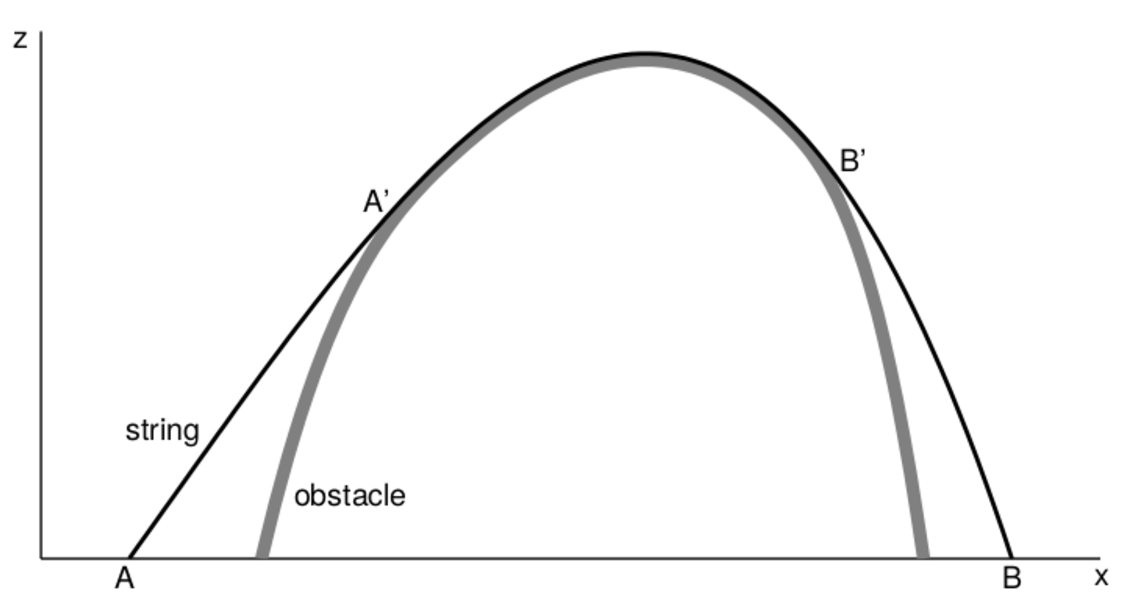
\includegraphics[scale=0.3]{image_obstacle}
\end{minipage}

\invisible<3>{
}}}
\end{frame}
%%%%%%%%%%%%
\begin{frame}
  \textcolor{midnightblue}{\textbf{Signorini problem:}}
  $\partial \Omega = \Gamma_{\mathrm{D}} \cup \Gamma_{\mathrm{N}} \cup \Gamma_{\mathrm{C}}$. \\
  $\Gamma_{\mathrm{D}}$: Dirichlet boundary conditions, $\Gamma_{\mathrm{N}}$: Neumann boundary conditions \\
  $\Gamma_{\mathrm{C}}$: Unilateral contact boundary conditions
  \\
  \vspace*{0.1 cm}
  Find $\textcolor{red}{\bu} \in \Kg := \left\{ \bv \in [H^1(\Omega)]^2 \ \text{s.t.} \ \bv=g \ \text{on} \ \Gamma_{\mathrm{D}}, \ \text{and} \ \bv\cdot \bn \leq 0 \ \text{on} \ \Gamma_{\mathrm{C}} \right\}$ such that
\begin{equation*}
\left( \sigma (\textcolor{red}{\bu}), \epsilon (\bv-\textcolor{red}{\bu}) \right)_{\Omega} \geq \left(\bbf,\bv-\textcolor{red}{\bu}\right)_{\Omega} + \left({\bm g}_{N}, \bv-\textcolor{red}{\bu} \right)_{\Gamma_{\mathrm{N}}}\quad \forall \bv \in \Kg
\end{equation*}

\begin{minipage}{0.55 \linewidth}
\begin{itemize}
\item $g \in H^{\frac{1}{2}}(\Gamma_{\mathrm{D}})$ : Dirichlet boudary datum for $\textcolor{red}{u}$
  \item  ${\bm g}_{\mathrm{N}} \in [L^2(\Gamma_{\mathrm{N}})]^2$ :  Neumann boundary data
  \item  $f \in [L^2(\Omega)]^2$: force acting on the solid elastic.
\end{itemize}
\end{minipage}
\hfill
\begin{minipage}{0.42 \linewidth}
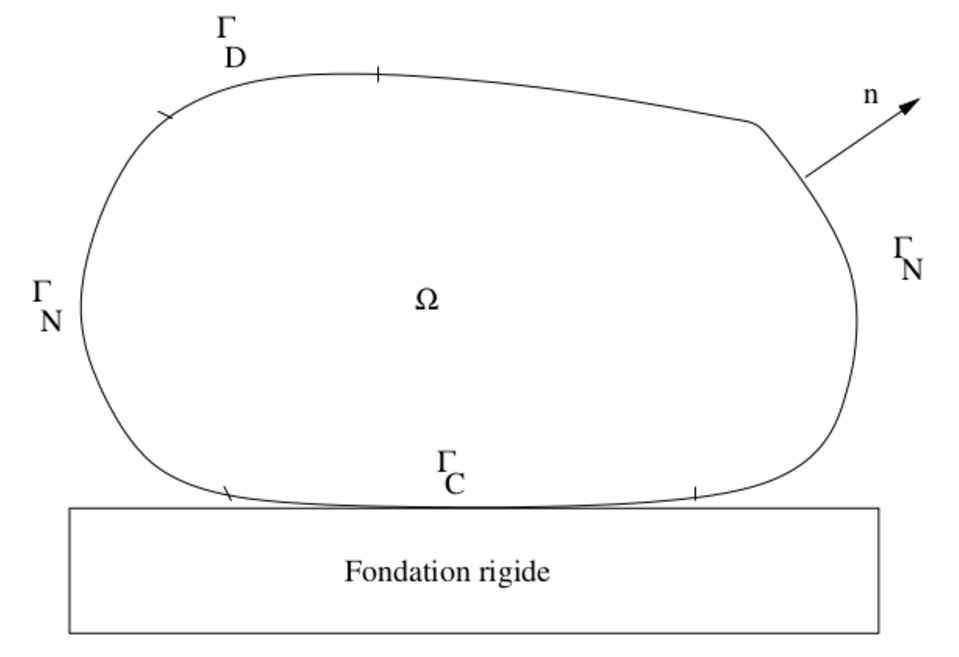
\includegraphics[scale=0.4]{image_signorini}
\end{minipage}
\end{frame}
\begin{frame}
\textcolor{midnightblue}{\textbf{Contact between two membranes:}}
\\
\vspace*{0.1 cm}
Find $\textcolor{red}{\bu}:=(\textcolor{red}{u_1},\textcolor{red}{u_2}) \in \Kg := \left\{ \bv = \left(v_1,v_2\right) \in H_{g_1}^1(\Omega) \times H_{g_2}^1(\Omega) \ \text{s.t.} \ v_1 - v_2 \geq 0  \ \text{a.e.} \ \text{in} \ \Omega \right\}$ such that
 \begin{equation*}
  \fbox{$ \sum_{\alpha=1}^2 \mu_{\alpha}
   \left( \nab \textcolor{red}{u_{\alpha}}, \nab \left(v_{\alpha} - \textcolor{red}{u_{\alpha}} \right) \right)_{\Omega} \geq
   \sum_{\alpha=1}^2 \left(f_{\alpha}, v_{\alpha} - \textcolor{red}{u_{\alpha}} \right)_{\Omega} \quad \forall \bv \in \Kg$ }
 \end{equation*}
 \begin{minipage}{0.37 \linewidth}
 \begin{itemize}
 \item $\mu_1, \mu_2$: tensions of the membranes
   \item $g_1 \geq g_2$ : boundary data
\end{itemize} 
 \end{minipage}
 \hfill
 \begin{minipage}{0.55 \linewidth}
\begin{figure}
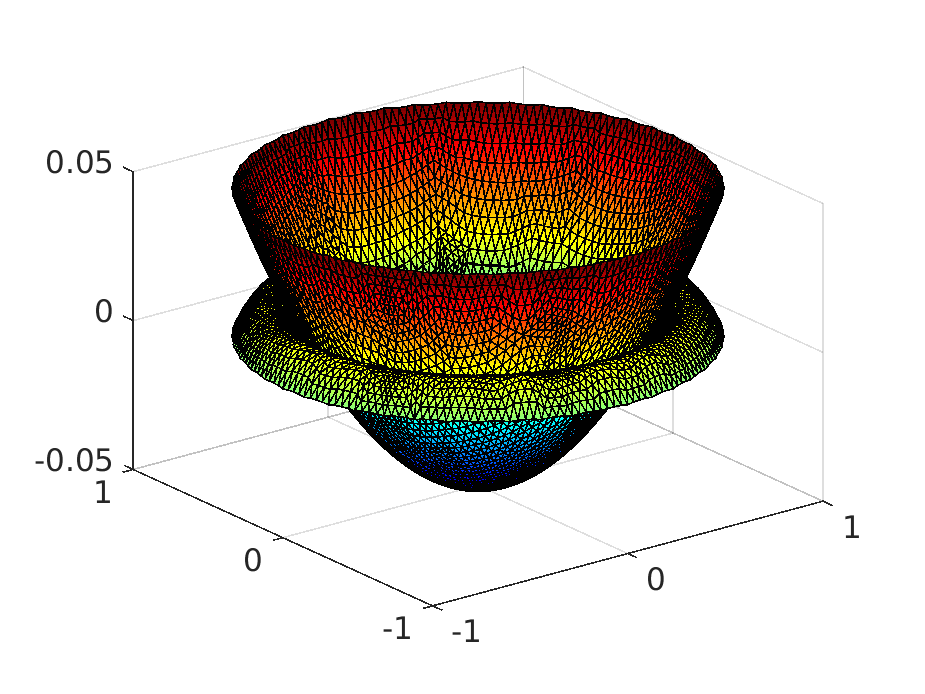
\includegraphics[scale = 0.5]{fig_article_chap_1/fig_membrane_cv.eps}    
\end{figure}
\end{minipage}

 \end{frame}
%%%%

%%%%%%%%%%%%%%%%%
\begin{frame}
\vspace*{0.1 cm}
\textcolor{red}{\textbf{Study the contact problem between two membranes}}
\\
\vspace{0.3 cm}
\textcolor{cadmiumgreen}{\textbf{Propose robust algorithms}}
\begin{itemize}
\item Discretization by the finite element method, the discontinuous Galerkin method, the hybrid high-order method
\end{itemize}
\textcolor{cadmiumgreen}{\textbf{Nonlinear resolution}}
\begin{itemize}
\item Semismooth Newton methods
  \end{itemize}
\textcolor{cadmiumgreen}{\textbf{Quantify the error}}
\begin{itemize}
  \item A posteriori error estimates
  \item Distinction of each error components
\end{itemize}

\textcolor{cadmiumgreen}{\textbf{Save computational time}}
\begin{itemize}
\item Adaptivity
  \end{itemize}
  \invisible<1>{
  \textcolor{red}{\textbf{Extension to unsteady problems?}}
  \invisible<2>{
  }}
\end{frame}



%%%%%%%%%%%%%%%%%%%%%%%%%%%%%
%% CHAP 1

\section{Model problem and discretization}
\subsection{}

%%%%%% PART 1%%%%%%%

\begin{frame}
\frametitle{Model problem and settings: contact between two membranes}
\vspace{-1.7 cm}
\begin{equation*}
\mbox{Find} \ u_1, u_2, \lambda \ \mbox{such that} \quad
\dps
\left\lbrace\begin{array}{llccc}
\dps -\mu_1 \Delta u_1-\lambda = f_1 \qquad \mbox{in} \quad \Omega, \\
\dps -\mu_2 \Delta u_2+\lambda = f_2 \qquad \mbox{in} \quad \Omega,\\
\textcolor{electricpurple}{u_1-u_2 \geq 0}, \quad 
\textcolor{carmine}{\lambda \geq 0}, \quad \dps (\textcolor{electricpurple}{u_1-u_2})\textcolor{carmine}{\lambda}=0 \quad \mbox{in} \quad \Omega, \hspace{0.2 cm}\\
\dps u_1=g_1, \ u_2=g_2  \qquad \mbox{on} \quad\partial \Omega.
\end{array}
\right.
\end{equation*}
\vspace{-0.8 cm}
\begin{figure}
\begin{subfigure}[normal]{0.44\textwidth} 
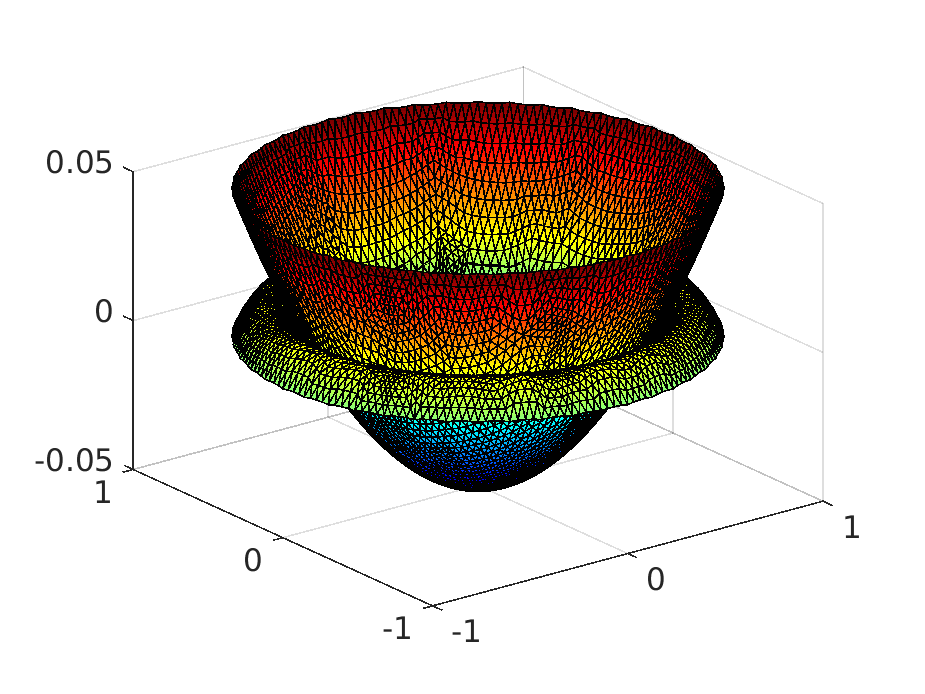
\includegraphics[width=\textwidth]{fig_article_chap_1/fig_membrane_cv.eps}    
\end{subfigure}
\qquad
\begin{subfigure}[normal]{0.44\textwidth}
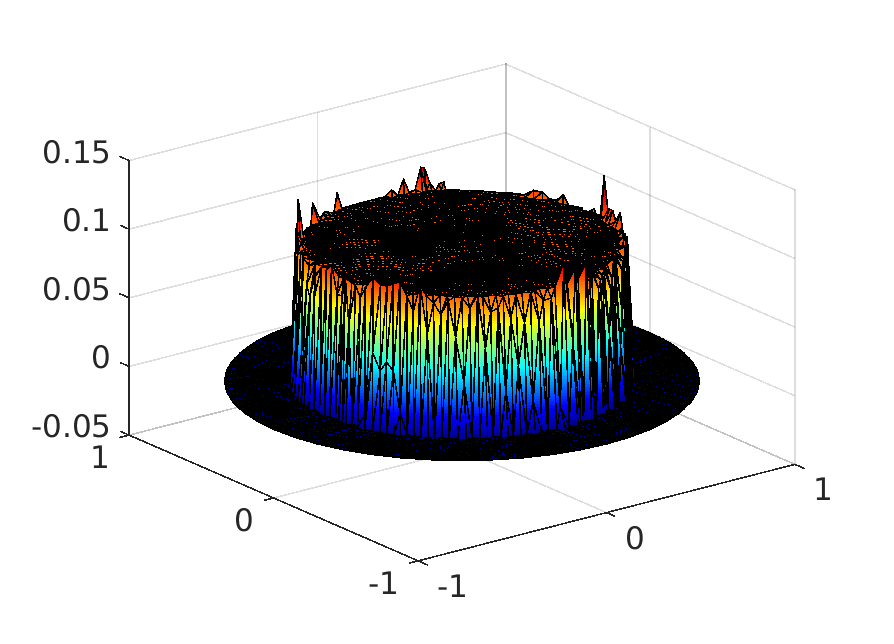
\includegraphics[width=\textwidth]{fig_article_chap_1/fig_lambda_cv.eps}     
\end{subfigure}
\end{figure}
\vspace*{-4.4cm}\hspace*{1.5 cm}$u_1$ \hspace{8 cm} $\lambda$\\
\vspace*{0.7cm}\hspace*{1.5 cm}$u_2$\\
\end{frame}
%%%%%
\begin{frame}
\frametitle{Continuous problem}
\begin{itemize}
\item $H_{g_{\alpha}}^1(\Omega) =  \left\{u\in H^1(\Omega), \hspace{0.1 cm} u=g_{\alpha} \hspace{0.1 cm} \mbox{on} \hspace{0.1 cm} \partial \Omega\right\}$ \quad $\Lambda=\left\{\chi\in L^2(\Omega), \: \textcolor{carmine}{\chi \geq 0} \: \mbox{a.e.} \hspace{0.1 cm} \mbox{in} \ \Omega\right\}$
\end{itemize}
\textbf{Saddle point type weak formulation:}
For $(f_1,f_2)\in \left[L^2(\Omega)\right]^2$ and $g > 0$ find $(u_1,u_2,\lambda)\in H_{g_1}^1(\Omega) \times H_{g_2}^1(\Omega) \times \Lambda$ such that
\begin{equation*}
\begin{split}
& \dps \sum_{\ialf=1}^2 \mu_\ialf \left(\nab u_\ialf,\nab v_\ialf\right)_{\Omega} - \left(\lambda,v_1-v_2\right)_{\Omega} = \sum_{\ialf=1}^2\left(f_\ialf,v_\ialf\right)_{\Omega} \quad \forall (v_1,v_2) \in \left[H_0^1(\Omega)\right]^2 \\
& \left(\chi - \textcolor{carmine}{\lambda},\textcolor{electricpurple}{u_1-u_2}\right)_{\Omega} \geq 0 
\quad \forall \chi \in \Lambda 
\end{split}
 \tag{$\textcolor{electricpurple}{\mathrm{S}}$}
\end{equation*}
\invisible<1>{
\hspace{4.5 cm}\textcolor{cadmiumgreen}{\textbf{equivalent to}}\\
\invisible<2>{
\textbf{Variational inequality:}
\vspace*{0.2 cm}
\begin{itemize}
\item $\Kg:= \left\{(v_1,v_2)\in H_{g_1}^1(\Omega)\times H_{g_2}^1(\Omega),\: \textcolor{electricpurple}{v_1-v_2 \geq 0} \; \; \mbox{a.e.} \ \mbox{in} 
\hspace{0.1 cm} \Omega \right\}$ \textcolor{midnightblue}{\textbf{convex}}
\end{itemize}
\begin{equation*}
\mbox{Find} \ \bu=\left(u_1,u_2\right) \in \Kg \ \mbox{s.t.} \ \dps \sum_{\ialf=1}^2 \mu_\ialf \left(\nab u_\ialf,\nab \left(v_\ialf-u_\ialf\right)\right)_{\Omega} \geq \sum_{\ialf=1}^2\left(f_\ialf,v_\ialf-u_\ialf\right)_{\Omega} \quad \forall \bv \in \Kg  \tag{$\textcolor{electricpurple}{\mathrm{R}}$}
\end{equation*}
\invisible<3>{
}}}
\end{frame}
%%%%%
\begin{frame}
\textcolor{red}{\textbf{For any $p \geq 1$}}
\\
\frametitle{The finite element method}
\textcolor{cadmiumgreen}{\textbf{Spaces for the discretization:}}\\
$X_{g_{\alpha}h}^p=\left\{v_h \in \mathcal{C}^0(\overline{\Omega}),  {v_h}_{|K} \in \Pp (K), \ \forall K \in {\mathcal{T}}_h, \hspace{0.2 cm} v_h=g_\alpha \hspace{0.2 cm} \mbox{on} \hspace{0.2 cm} \partial \Omega\right\}$\\
\vspace*{0.3 cm}
$\Xzerohp =\left\{v_h \in \calC^0(\overline{\Omega}); \ {v_h}|_{K} \in \Pp (K), \ \forall K \in \Th, \hspace{0.2 cm} v_h=0 \hspace{0.2 cm} \mbox{on} \hspace{0.2 cm} \partial \Omega \right\}$
\\
\vspace*{0.3 cm}
$\dps \Kghp=\left\{(\vunh,\vdeuxh) \in X_{g_1 h}^p \times X_{g_2 h}^p, \ \textcolor{electricpurple}{\vunh(\xl)-\vdeuxh(\xl)} \geq 0 \ \ \forall \xl \in \Vdp \right\} \textcolor{red}{\not \subset \Kg \quad \forall p \geq 2}$\\
\vspace*{0.2 cm}
\invisible<1>{
\textcolor{cadmiumgreen}{\textbf{Discrete variational inequality:}} find $\dps \uh=(\uunh,\udeuxh) \in \Kghp$ such that
\begin{equation*}
\dps \sum_{\ialf=1}^2 \mu_\ialf \left(\nab u_{\ialf h},\nab \left(v_{\ialf h}-u_{\ialf h}\right)\right)_{\Omega} \geq \sum_{\ialf=1}^2\left(f_\ialf,v_{\ialf h}-u_{\ialf h}\right)_{\Omega} \quad \forall \bv_h = (v_{1h},v_{2h})\in ~\Kghp \quad \textcolor{electricpurple}{(\mathrm{DR})}
\end{equation*}
\begin{center}
\textcolor{midnightblue}{Well-posed problem (Lions--Stampacchia)}
\end{center}
\invisible<2>{
\textcolor{midnightblue}{\textbf{Resolution techniques:}}
\footnotesize{Projected Newton methods (Bertsekas 1982), Active set Newton method (Kanzow 1999), Primal-dual active set strategy (Hinterm\"uller 2002).}
\invisible<3>{
}}}
\end{frame}
%
\begin{frame}
  \textcolor{red}{\textbf{Saddle point formulation}}
  \\
  \vspace*{0.2 cm}
\only<1>{
\textcolor{midnightblue}{\textbf{Discretization of}} $\Lambda=\left\{\chi\in L^2(\Omega), \: \textcolor{carmine}{\chi \geq 0} \: \mbox{a.e.} \ \mbox{in} \hspace{0.1 cm} \Omega\right\}$
\\
\vspace{0.4 cm}
\textcolor{red}{\textbf{$p = 1$:}} \ $\Lahone \egaldef \left\{v_h \in \Xzerohone \  \textcolor{carmine}{v_h(\ba)} \geq 0 \ \forall \ba \in \mathcal{V}_{d}^{\mathrm{int}} \right\} \textcolor{red}{\bm \subset \bm \Lambda}$ \scriptsize{Ben Belgacem, Bernardi, Blouza, and Vohral{\'{\i}}k (2012)}.\\
\vspace{0.4 cm}
\normalsize{\textcolor{red}{\textbf{$p \geq 2$ (\textcolor{cadmiumgreen}{\textbf{new}}):}} \ $\Lahp \egaldef \left\{v_h \in \XXhp \ \left(v_h ,\psihl \right)_{\Omega} \geq 0 \ \forall \xl \in \Vdpint \ \left(v_h,\psihl\right)_{\Omega} = 0 \hspace{0.05 cm} \forall \xl \in \Vdpext\right\}$ $\textcolor{red}{\bm \not \subset \bm \Lambda}$}
\vspace{0.4 cm}
\begin{equation*}
\left\langle w_h ,v_h \right\rangle_h \egaldef \dps \sum_{\ba \in \Vh} w_h(\ba) v_h(\ba) \left(\psiha,1\right)_{\omah}  \quad \mbox{if} \quad \textcolor{red}{\textbf{$p=1$}} \quad \mbox{and} \quad \left \langle w_h ,v_h \right\rangle_h  \egaldef \dps \left(w_h, v_h\right)_{\Omega} \quad \mbox{if} \quad \textcolor{red}{\textbf{$p \geq 2$}}
\end{equation*}
% \vspace{0.2 cm}
% \textcolor{cadmiumgreen}{\textbf{Continuous weak formulation}}
% \begin{equation*}
% \begin{split}
% & \dps \sum_{\ialf=1}^2 \mu_\ialf \left(\nab u_\ialf,\nab v_\ialf\right)_{\Omega} - \left(\lambda,v_1-v_2\right)_{\Omega} = \sum_{\ialf=1}^2\left(f_\ialf,v_\ialf\right)_{\Omega} \quad \forall (v_1,v_2) \in \left[H_0^1(\Omega)\right]^2 \\
% & \left(\chi - \textcolor{carmine}{\lambda},\textcolor{electricpurple}{u_1-u_2}\right)_{\Omega} \geq 0 
% \quad \forall \chi \in \Lambda 
% \end{split}
%  \tag{$\textcolor{electricpurple}{\mathrm{S}}$}
% \end{equation*}
}
\only<2>{
Recall $\Lambda=\left\{\chi\in L^2(\Omega), \: \textcolor{carmine}{\chi \geq 0} \: \mbox{a.e.} \ \mbox{in} \hspace{0.1 cm} \Omega\right\}$
\\
\vspace{0.4 cm}
\textcolor{red}{\textbf{$p = 1$:}} \ $\Lahone \egaldef \left\{v_h \in \Xzerohone \  \textcolor{carmine}{v_h(\ba)} \geq 0 \ \forall \ba \in \mathcal{V}_{d}^{1,\mathrm{int}} \right\} \textcolor{red}{\bm \subset \bm \Lambda}$ \scriptsize{Ben Belgacem, Bernardi, Blouza, and Vohral{\'{\i}}k (2012)}.\\
\vspace{0.4 cm}
\normalsize{\textcolor{red}{\textbf{$p \geq 2$ (\textcolor{cadmiumgreen}{\textbf{new}}):}} \ $\Lahp \egaldef \left\{v_h \in \XXhp \ \left(v_h ,\psihl \right)_{\Omega} \geq 0 \ \forall \xl \in \Vdpint \ \left(v_h,\psihl\right)_{\Omega} = 0 \hspace{0.05 cm} \forall \xl \in \Vdpext\right\}$ $\textcolor{red}{\bm \not \subset \bm \Lambda}$} 
\vspace{0.4 cm}
\begin{equation*}
\left\langle w_h ,v_h \right\rangle_h \egaldef \dps \sum_{\ba \in \Vh} w_h(\ba) v_h(\ba) \left(\psiha,1\right)_{\omah}  \quad \mbox{if} \quad \textcolor{red}{\textbf{$p=1$}} \quad \mbox{and} \quad \left \langle w_h ,v_h \right\rangle_h  \egaldef \dps \left(w_h, v_h\right)_{\Omega} \quad \mbox{if} \quad \textcolor{red}{\textbf{$p \geq 2$}}
\end{equation*}
\vspace{0.2 cm}
\textcolor{cadmiumgreen}{\textbf{Continuous weak formulation}}
\begin{equation*}
\begin{split}
& \dps \sum_{\ialf=1}^2 \mu_\ialf \left(\nab u_\ialf,\nab v_\ialf\right)_{\Omega} - \left(\lambda,v_1-v_2\right)_{\Omega} = \sum_{\ialf=1}^2\left(f_\ialf,v_\ialf\right)_{\Omega} \quad \forall (v_1,v_2) \in \left[H_0^1(\Omega)\right]^2 \\
& \left(\chi - \textcolor{carmine}{\lambda},\textcolor{electricpurple}{u_1-u_2}\right)_{\Omega} \geq 0 
\quad \forall \chi \in \Lambda 
\end{split}
 \tag{$\textcolor{electricpurple}{\mathrm{S}}$}
\end{equation*}
}

\only<3>{
Recall $\Lambda=\left\{\chi\in L^2(\Omega), \: \textcolor{carmine}{\chi \geq 0} \: \mbox{a.e.} \ \mbox{in} \hspace{0.1 cm} \Omega\right\}$
\\
\vspace{0.4 cm}
\textcolor{red}{\textbf{$p = 1$:}} \ $\Lahone \egaldef \left\{v_h \in \Xzerohone \  \textcolor{carmine}{v_h(\ba)} \geq 0 \ \forall \ba \in \mathcal{V}_{d}^{1,\mathrm{int}} \right\} \textcolor{red}{\bm \subset \bm \Lambda}$ \scriptsize{Ben Belgacem, Bernardi, Blouza, and Vohral{\'{\i}}k (2012)}.\\
\vspace{0.4 cm}
\normalsize{\textcolor{red}{\textbf{$p \geq 2$ (\textcolor{cadmiumgreen}{\textbf{new}}):}} \ $\Lahp \egaldef \left\{v_h \in \XXhp \ \left(v_h ,\psihl \right)_{\Omega} \geq 0 \ \forall \xl \in \Vdpint \ \left(v_h,\psihl\right)_{\Omega} = 0 \hspace{0.05 cm} \forall \xl \in \Vdpext\right\}$ $\textcolor{red}{\bm \not \subset \bm \Lambda}$} 
\vspace{0.4 cm}
\begin{equation*}
\left\langle w_h ,v_h \right\rangle_h \egaldef \dps \sum_{\ba \in \Vh} w_h(\ba) v_h(\ba) \left(\psiha,1\right)_{\omah}  \quad \mbox{if} \quad \textcolor{red}{\textbf{$p=1$}} \quad \mbox{and} \quad \left \langle w_h ,v_h \right\rangle_h  \egaldef \dps \left(w_h, v_h\right)_{\Omega} \quad \mbox{if} \quad \textcolor{red}{\textbf{$p \geq 2$}}
\end{equation*}
\vspace{0.2 cm}
\textcolor{cadmiumgreen}{\textbf{Discrete weak formulation}}
Find $(\uunh,\udeuxh,\lambh)\in X_{g_1 h}^p \times X_{g_2 h}^p \times \Lahp$ s.t.  
\vspace{-0.3 cm}
\begin{equation*}
\begin{split}
& \sum_{\ialf=1}^2 \mu_\ialf \left(\nab u_{\ialf h}, \nab z_{\ialf h}\right)_{\Omega}
- \left\langle \lambh, z_{1h}-z_{2h} \right \rangle_h
= \sum_{\ialf=1}^2 \left(f_\ialf,z_{\ialf h}\right)_{\Omega}, \quad \forall(z_{1h},z_{2h})\in [\Xzerohp]^2 \\
& \left\langle \chi_h - \textcolor{carmine}{\lambh}, \textcolor{electricpurple}{\uunh - \udeuxh}\right \rangle_h   \geq 0 \quad \forall \chi_h \in \Lahp.
\end{split}
 \tag{$\textcolor{electricpurple}{\mathrm{DS}}$}
\end{equation*}
}
\end{frame} 
%

\begin{frame}
 \textcolor{red}{\textbf{Discrete complementarity problem}}
%\frametitle{Discrete complementarity problems}
\vspace*{-0.2 cm}
\begin{equation*}
\begin{array}{lcl}
\dps \sum_{\ialf=1}^2 \mu_\ialf \left(\nab u_{\ialf h}, \nab z_{\ialf h}\right)_{\Omega}
- \left\langle \lambh, z_{1h}-z_{2h} \right \rangle_h
=  \dps \sum_{\ialf=1}^2 \left(f_\ialf,z_{\ialf h}\right)_{\Omega} \quad \forall(z_{1h},z_{2h})\in [\Xzerohp]^2, \\
\textcolor{electricpurple}{\left(\uunh-\udeuxh \right)(\xl)} \geq 0 \ \forall \xl \in \Vdpint, \ \left\langle \textcolor{carmine}{\lambh}, \psihl \right \rangle_h \geq 0 \ \forall \xl \in \Vdpint, \ \left\langle \textcolor{carmine}{\lambh}, \textcolor{electricpurple}{\uunh - \udeuxh} \right \rangle_h=0.  \quad \textcolor{electricpurple}{(\mathrm{DS}2)}
\end{array}
\end{equation*}
\invisible<1>{
\textcolor{cadmiumgreen}{\textbf{Matrix representation of \textcolor{electricpurple}{($\mathrm{DS}2)$}}}
\newline
\newline
\invisible<2>{
\textcolor{red}{\textbf{$p \geq 1$:}}
$\dps \uunh = \sum_{l=1}^{\Ndpint} \left(\X_{1h} \right)_l \psihl, \quad \udeuxh = \sum_{l=1}^{\Ndpint} \left(\X_{2h} \right)_l \psihl \quad \lambh = \sum_{l=1}^{\Ndpint} \left(\X_{3h} \right)_l \Thetahl.$ 
\begin{equation*}
\begin{split}
&\bbE \Xh = \bF,\\
&\textcolor{electricpurple}{\X_{1h} - \X_{2h}} \geq 0, \quad \textcolor{carmine}{\X_{3h}} \geq 0, \quad \left(\textcolor{electricpurple}{\X_{1h} - \X_{2h}} \right) \cdot \textcolor{carmine}{\X_{3h}} = 0.
\end{split}
\qquad 
\bbE
\egaldef
\left[\begin{array}{ccr}
\mu_1 \bbS & \mathbf{0} & -\mathbb{D} \\
\mathbf{0} &\mu_2 \bbS & + \mathbb{D}
\end{array}
\right]
\end{equation*}
\invisible<3>{
}}}
\end{frame}
%
\begin{frame}
  \frametitle{The Discontinuous Galerkin method}
  \textcolor{cadmiumgreen}{\textbf{Discontinuous spaces:}}
  \begin{equation*}
    \begin{split}
      X_h^p &:= \left\{ v_h \in L^2(\Omega) \ \text{s.t.} \ v_h|_{K} \in \mathbb{P}_p(K) \ \forall K \in \Th \right\} \\
      X_{g_{\alpha} h}^p &:= \left\{ v_h \in L^2(\Omega) \ \text{s.t.} \ v_h|_{K} \in \mathbb{P}_p(K) \ \forall K \in \Th \ \text{and} \ v_h=g_{\alpha} \ \text{on} \ \partial \Omega \right\} \\
       \Kghp & := \left\{ \bv_h := \left(v_{1h},v_{2h}  \right) \in X_{g_{1} h}^p \times X_{g_{2} h}^p \ \text{s.t.} \ \left(v_{1h} - v_{2h}\right)|_{K}(\bx_l) \geq 0 \ \forall \bx_l \in \VKint \ \forall K \in \Th \right\}
    \end{split}
  \end{equation*}
  \textcolor{cadmiumgreen}{\textbf{Discrete variational inequality:}} find $\dps \uh=(\uunh,\udeuxh) \in \Kghp$ such that
\begin{equation*}
\dps \sum_{\alpha=1}^2 \mu_{\alpha} \mathcal{A}_h(u_{\alpha h}, v_{\alpha h} - u_{\alpha h}) \geq \sum_{\ialf=1}^2 \sum_{K \in \Th} \left(f_\ialf|_K,v_{\ialf h}|_K-u_{\ialf h}|_K\right)_{K} \quad \forall \bv_h = (v_{1h},v_{2h})\in ~\Kghp \quad \textcolor{electricpurple}{(\mathrm{DR})}
\end{equation*}
$\mathcal{A}_h$ : bilinear form $a$ + consistency and stability terms [SIPG, NIPG]
\vspace*{0.2 cm}
  \begin{center}
\textcolor{midnightblue}{Well-posed problem (Lions--Stampacchia)}
\end{center}
\end{frame}
%%%%
\begin{frame}
  \textcolor{red}{\textbf{Discrete complementarity problem}}
  \\
    \begin{align*}
\Lahp &  := \left\{ v_h \in X_h^p \ \text{s.t.} \ \left(v_h|_{K}, \psihl|_K \right)_K \geq 0 \ \forall K \in \Th, \ \forall \bx_l \in \VKint, \ \text{and} \left(v_h|_K, \psihl|_K  \right)_K = 0 \right. \\
       & \left.  \forall K \in \Th \ \forall \bx_l \in \VKext \right\}    \qquad \textcolor{red}{p \geq 2}
  \end{align*}
Find $\left(u_{1h}, u_{2h}, \lambda_h\right) \in X_{g_1 h}^p \times X_{g_2 h}^p \times \Lahp$ such that
\begin{equation*}
\begin{array}{lcl}
\dps \dps \sum_{\alpha=1}^2 \mu_{\alpha} \mathcal{A}_h(u_{\alpha h}, v_{\alpha h}) - \sum_{K \in \Th} \left(v_{1h}|_K - v_{2h}|_K, \lambda_h|_K \right)_K 
=  \dps \sum_{\ialf=1}^2 \sum_{K \in \Th} \left(f_\ialf|_K,v_{\ialf h}|_K \right)_{K} \quad \forall \bv_h \in \left[X_{0 h}^p\right]^2, \\
\textcolor{electricpurple}{\left(\uunh|_K-\udeuxh|_K \right)(\xl)} \geq 0 \ \forall \xl \in \Vdpint, \ \left(\textcolor{carmine}{\lambh|_K}, \psihl \right) \geq 0 \ \forall \xl \in \Vdpint, \ \left( \textcolor{carmine}{\lambh|_K}, \textcolor{electricpurple}{\uunh|_K - \udeuxh|_K} \right)=0.  \quad \textcolor{electricpurple}{(\mathrm{DS}2)}
\end{array}
\end{equation*}
\invisible<1>{
\textcolor{cadmiumgreen}{\textbf{Matrix representation}} $\Xh:=\left[\X_{1h}, \X_{2h}, \X_{3h}\right] \in \mathbb{R}^{3 \Nhint}$
\newline
\invisible<2>{
\begin{equation*}
\begin{split}
&\bbE \Xh = \bF,\\
&\textcolor{electricpurple}{\X_{1h} - \X_{2h}} \geq 0, \quad \textcolor{carmine}{\X_{3h}} \geq 0, \quad \left(\textcolor{electricpurple}{\X_{1h} - \X_{2h}} \right) \cdot \textcolor{carmine}{\X_{3h}} = 0.
\end{split}
\qquad 
\bbE
\egaldef
\left[\begin{array}{ccr}
\mu_1 \bbS & \mathbf{0} & -\mathbb{D} \\
\mathbf{0} &\mu_2 \bbS & + \mathbb{D}
\end{array}
\right]
\end{equation*}
\invisible<3>{
}}}
\end{frame}
%%%
\begin{frame}
  \frametitle{The Hybrid High-Order method}
  The unknowns are polynomial
  functions attached to the cells and the edges of the mesh. The polynomials attached to the cells can be eliminated through a static condensation procedure.
  \begin{center}
\hspace{2 cm} FEM \qquad \qquad HHO without SC \qquad  HHO with SC 
    \end{center}
  \begin{figure}
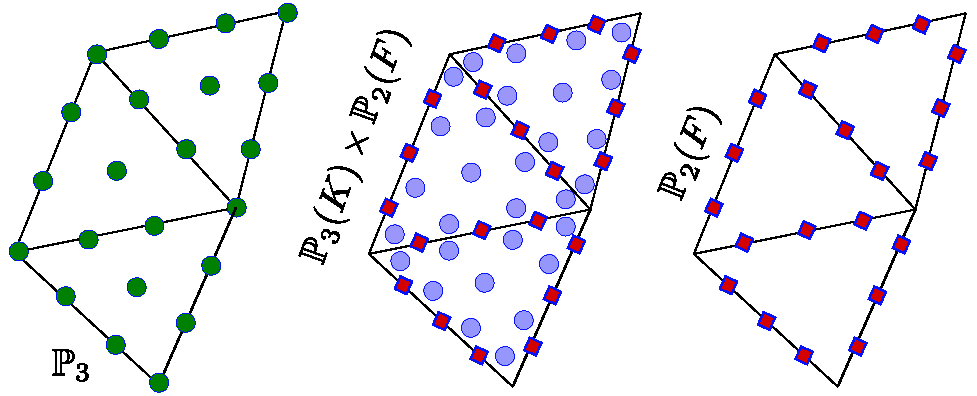
\includegraphics[width=0.55\textwidth]{HHO_FEM}
%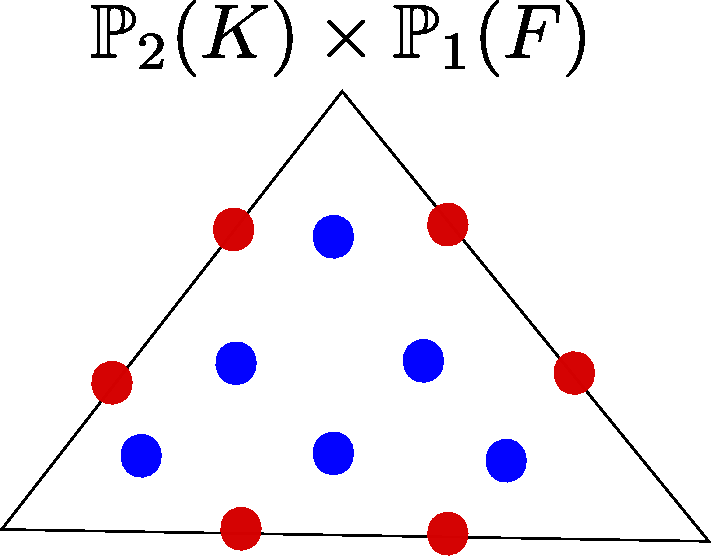
\includegraphics[width=0.32\textwidth]{HHO_P2_P1}
%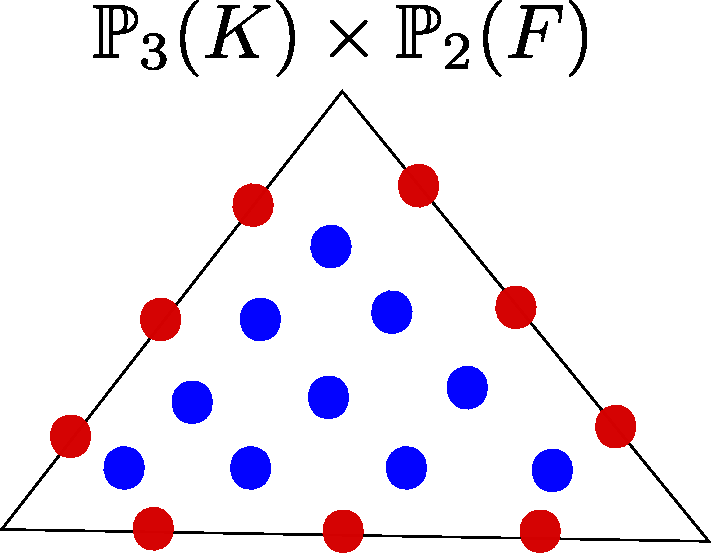
\includegraphics[width=0.32\textwidth]{HHO_P3_P2}
  \end{figure}
  \textcolor{cadmiumgreen}{\textbf{The blue DOFs are eliminated!}}
  
   \scriptsize{ \textcolor{midnightblue}{\textbf{HHO papers:}} Di Pietro, Ern (2015), Cockburn, Di Pietro, Ern (2016), Cascavita, Chouly, Ern (2019), Cicuttin, Ern, Gudi (2020), Chouly, Ern, Pignet (2020)}
\end{frame}
%%%%
\begin{frame}
  \textcolor{cadmiumgreen}{\textbf{Discontinuous spaces:}} \hspace{4 cm} 
  $\Eh$ : \textcolor{midnightblue}{set of edges}, \ $\mathcal{V}_K$ : \textcolor{midnightblue}{DOFs in a triangle}
    \begin{equation*}
    \begin{split}
      X_h^p &:= \prod_{K \in \Th} \mathbb{P}_p(K) \times \prod_{F \in \Eh} \mathbb{P}_{p-1}(F), \quad \\
      X_{g_{\alpha} h}^p &:= \left\{ v_h \in  X_h^p \ \text{s.t.} \ v_h=g_{\alpha} \ \text{on} \ \partial \Omega \right\}: \ \textcolor{red}{u_1, u_2} 
      %\Lambda_h := \prod_{K \in \Th} \mathbb{P}_p(K): \ \textcolor{red}{\lambda}
      \\
       \Kghp & := \left\{ \bv_h := \left(v_{1h},v_{2h}  \right) \in X_{g_1 h}^p \times X_{g_2 h}^p \ \text{s.t.} \ \left(v_{1h} - v_{2h}\right)|_{K}(\bx_l) \geq 0 \ \forall \bx_l \in \VK \ \forall K \in \Th \right\}
    \end{split}
    \end{equation*}
%    \textcolor{cadmiumgreen}{\textbf{Gradient reconstruction operator in every cell}:} 
%$\bG_K : X_{h,K}^p \to \polP_p(K;\R^2)$ such that
%\begin{equation*}
%  ( \bG_K(\hv_K) , \bq )_{K} \egaldef (\nab v_K , \bq )_K 
%  + \sum_{F \in \EK} (v_{F} - v_K , \bq \SCAL \bn_K)_{F} , \quad \forall \hv_K \in X_{h,K}^p, \quad \forall \bq \in \polP_p(K;\R^2),
%\end{equation*}

\textcolor{cadmiumgreen}{\textbf{Bilinear form:}} 
Gradient reconstruction operator $+$ projection term 
%$\forall \hv_h \in X_h^p$, $\forall \hw_h \in X_h^p$
%\begin{equation*}
%  \begin{split}
%  \mathcal{A}_h(\hv_h , \hw_h) \egaldef
%  \sum_{K \in \Th} \Big(
%  \left(\bG_K(\hv_{K}) , \bG_K(\hw_{K})\right)_{K}
%  + h_K^{-1} \sum_{F \in \EK} \left(\Pi_{F}^{p-1}(v_{K} - v_{F}) , w_{K} - w_{F}\right)_{F} 
%  \Big) ,
%\end{split}
%\end{equation*}
\\
 \textcolor{cadmiumgreen}{\textbf{Discrete variational inequality:}} find $\dps \uh=(\uunh,\udeuxh) \in \Kghp$ such that
\begin{equation*}
\dps \sum_{\alpha=1}^2 \mu_{\alpha} \mathcal{A}_h(u_{\alpha h}, v_{\alpha h} - u_{\alpha h}) \geq \sum_{\ialf=1}^2 \sum_{K \in \Th} \left(f_\ialf|_K,v_{\ialf h}|_K-u_{\ialf h}|_K\right)_{K} \quad \forall \bv_h = (v_{1h},v_{2h})\in ~\Kghp \quad \textcolor{electricpurple}{(\mathrm{DR})}
\end{equation*}
 \begin{center}
\textcolor{midnightblue}{Well-posed problem (Lions--Stampacchia)}
\end{center}
\end{frame}
%%%%%%%%%%%
\begin{frame}
      
  \textcolor{red}{\textbf{HHO without static condensation:}}
  \begin{align*}
\bbE \egaldef 
\left[
  \begin{array}{ccccr}
    \mu_1 \bbS_{CC} 
    & \mu_1 \bbS_{CF} & \bf 0 & \bf 0 & -\mathbb{I}_d 
    \\
    \mu_1 \bbS_{FC} 
    & \mu_1 \bbS_{FF} & \bf 0 & \bf 0 & \bf 0
    \\
    \bf 0 & \bf 0 & \mu_2 \bbS_{CC} & \mu_2 \bbS_{CF} & \mathbb{I}_d
    \\
    \bf 0 & \bf 0 & \mu_2 \bbS_{FC} & \mu_2 \bbS_{FF} & \bf 0
  \end{array}
\right], \quad 
\bF \egaldef \left[\begin{array}{l} \bF_1 \\ \bf 0 \\ \bF_2 \\ \bf 0 \end{array} \right], \quad
%  \\
\X_h \egaldef \left[
  \begin{array}{l}\X_{1h}^{\mathrm{C}}\\ \X_{1h}^{\mathrm{F}} \\ \X_{2h}^{\mathrm{C}}\\ \X_{2h}^{\mathrm{F}} \\ \X_{3h} \end{array} \right] .
  \end{align*}
  \vspace*{-0.2 cm}
  %% \begin{itemize}
  %% \item  $\bF_\alpha \in \mathbb{R}^{m_c}, \ \X_{1h}^{\mathrm{C}} \in \mathbb{R}^{m_c}, \ \X_{2h}^{\mathrm{C}} \in \mathbb{R}^{m_c}, \ \X_{3h} \in \mathbb{R}^{m_c}$, $m_c = \frac{1}{2} (p+1)(p+2) \mathcal{N}_{\mathcal{T}}$
  %% \item $\X_{1h}^{\mathrm{F}} \in \mathbb{R}^{m_F}, \ \X_{2h}^{\mathrm{F}} \in \mathbb{R}^{m_F}$, $m_F := \mathcal{N}_{\varepsilon}^{\mathrm{int}} p$
  %% \end{itemize}
  \invisible<1>{
  \textcolor{red}{\textbf{Discrete complementarity problem}}
\newline
\begin{equation*}
\begin{split}
&\bbE \Xh = \bF,\\
&\textcolor{electricpurple}{\X_{1h}^{\mathrm{C}} - \X_{2h}^{\mathrm{C}}} \geq 0, \quad \textcolor{carmine}{\X_{3h}} \geq 0, \quad \left(\textcolor{electricpurple}{\X_{1h}^{\mathrm{C}} - \X_{2h}^{\mathrm{C}}} \right) \cdot \textcolor{carmine}{\X_{3h}} = 0.
\end{split}
\end{equation*}
\invisible<2>{
  \textcolor{red}{\textbf{Static condensation procedure:}} Later, need the semismooth resolution!
\invisible<3>{
}}}
\end{frame}
%%%%%%%%
\section{Semismooth Newton and first numerical results}
\subsection{}

\begin{frame}
\frametitle{C-functions}
\vspace{-0.2 cm}
\begin{definition}
$f: \left(\R^m\right)^2  \rightarrow \R^m$ ($m \geq 1$) is a
$C$-function or a complementarity function if
\begin{equation*}
\forall(\bx,\by)\in \left(\R^m\right)^2
\qquad f(\bx,\by)=\mathbf{0} \quad \iff \quad
\bx \geq \mathbf{0}, \quad \by \geq \mathbf{0}, \quad \bx {\cdot} \by=0.
\end{equation*}
\end{definition}
\invisible<1>{
\textcolor{cadmiumgreen}{\textbf{min function:}} \ $\left(\min \{\bx, \by\}\right)_l \egaldef \min \left\{\bx_l, \by_l\right\} \qquad l = 1,\dots, m$\\
\vspace{0.2 cm}
\invisible<2>{ \textcolor{cadmiumgreen}{\textbf{ Fischer--Burmeister function:}} \ $\left(f_{\mathrm{FB}}(\bx,\by)\right)_l \egaldef \sqrt{\bx_l^2+\by_l^2}-\left(\bx_l+\by_l\right) \quad  l = 1,\dots, m$
\\ 
\invisible<3>{$\bx=\textcolor{electricpurple}{\X_{1h} - \X_{2h}}$, \ $\by = \textcolor{carmine}{\X_{3h}}$, \ $\CFun(\X_{h})
= \tilde \CFun(\textcolor{electricpurple}{\X_{1h} - \X_{2h}}, \textcolor{carmine}{\X_{3h}})$. 
\begin{equation*}
\left\lbrace\begin{array}{llccc}
\bbE \X_{h} &= \bF,\\
\CFun(\X_{h})&=\mathbf{0}.
\end{array}
\right.
\end{equation*}
\invisible<4>{
\textcolor{red}{\textbf{The C-function is not Fréchet differentiable.}}\\
\vspace{0.2 cm}
\invisible<5>{
\textcolor{red}{\textbf{We will use semismooth Newton algorithms.}} 
\\
\scriptsize{Facchinei and Pang (2003), Bonnans, Gilbert, Lemar\'echal, and Sagastiz\'abal (2006).} 
\invisible<6>{
}}}}}}
\end{frame}
%
\begin{frame}
\frametitle{Inexact semismooth Newton method}
\textcolor{cadmiumgreen}{\textbf{Newton initial vector:}} $\Xh^{\zzero} \egaldef \left(\X_{1h}^{\zzero},\X_{2h}^{\zzero}, \X_{3h}^{\zzero} \right)^{T} \in \R^{3 m}$, on step $\kk \geq 1$, one looks for $\Xh^{\kk} \in \R^{3 m}$ such that
\begin{equation*}
\bbA^{\kk-1}\Xh^{\kk}=\bB^{\kk-1},
\end{equation*} 
where 
\begin{equation*}
\dps \bbA^{\kk-1}\egaldef
\left[\begin{array}{c}
\bbE \\
\JacCFun(\Xh^{\kk-1})
\end{array}
\right],
\quad  \hspace{0.1 cm} \bB^{\kk-1} \egaldef
\left[\begin{array}{c}
\bF\\
\JacCFun(\Xh^{\kk-1})\Xh^{\kk-1}-\CFun(\Xh^{\kk-1})
\end{array}
\right].
\end{equation*}
\textcolor{cadmiumgreen}{\textbf{Inexact solver initial vector:}}
$\Xh^{\kk,\izzero} \in \R^{3 m}$, often taken as $\Xh^{\kk,\izzero} = \Xh^{\kk-1}$, this yields on step $\ii \geq 1$
an approximation $\Xh^{\kk,\ii}$ to $\Xh^{\kk}$ satisfying
\begin{equation*}
\bbA^{\kk-1}\Xh^{\kk,\ii} =\bB^{\kk-1}-{\bm R}_h^{\kk,\ii},
\end{equation*}
where ${\bm R}_h^{\kk,\ii} \in \R^{3 m}$ is the algebraic residual vector.
\end{frame}
%%%%%%
%%%%%%
\begin{frame}
  \frametitle{Newton-min convergence}
  \begin{theorem}
    The Newton-min Algorithm is well defined.
    Moreover, if the first guess $\X_h^0$  is close enough to the solution $\X_h^*$ to the nonlinear system, then the sequence $\left(\Xh^{\kk}\right)_{\kk \geq 1}$ converges to $\X_h^*$ with a finite number of semismooth iterations and the local convergence is quadratic.

    In other words,
    \begin{equation*}
\begin{split}
  \left\| \X_h^{\kk} - \X_h^* \right\|_2 \leq K \left\| \X_h^{\kk-1} - \X_h^* \right\|_2^2,
\end{split}
\end{equation*}
  \end{theorem}

  \end{frame}
%%
\begin{frame}
  \frametitle{HHO with static condensation}
  \begin{itemize}
  \item
  Express the cell components from the face components by local problems
  \item
  By substitution derive from the global system the edge unknowns problem
  \item
  Recover the solution attached to the cells
  \item
  Important computational speed-up 
  \end{itemize}
\begin{table}
  \centering
  \begin{tabular}[h]{| c | c | c | c | c | c | c | c | c |}
    \hline
    &\multicolumn{2}{ c |}{$\polP_1$ DOFs} & \multicolumn{2}{ c |}{$\polP_2$ DOFs} 
    & \multicolumn{2}{ c |}{$\polP_3$ DOFs} & \multicolumn{2}{ c |}{$\polP_4$ DOFs}
    \\
    \hline
    Mesh  & no SC & SC & no SC & SC & no SC & SC & no SC & SC
    \\
    \hline
    $\mathcal{T}_0$   & 752   & 176   & 1504   & 352   & 2448   & 528    & 3584   & 704
    \\
    \hline
    $\mathcal{T}_1$   & 3040  & 736   & 6080   & 1472  & 9888   & 2208   & 14464  & 2944
    \\
    \hline
    $\mathcal{T}_2$ & 12224 & 3008  & 24448  & 6016  & 39744  & 9024   & 58112  & 12032
    \\
    \hline
    $\mathcal{T}_3$ & 49024 & 12160 & 98048  & 24320 & 159360 & 36480  & 232960 & 48640
    \\
    \hline
    $\mathcal{T}_4$ &196352 & 48896 & 392704 & 97792 & 638208 & 146688 & 932864 & 195584
    \\
    \hline
  \end{tabular}
\end{table}  
  \end{frame}
%%%%%%%%%%
\begin{frame}
  \frametitle{Numerical experiments}
  \begin{itemize}
  \item unit square domain $\Omega:=(0,1)\times(0,1)$
  \item We compare the performance of FEM and HHO
  \end{itemize}
  \textcolor{cadmiumgreen}{\textbf{First test case}}
\begin{equation*}
  u_1 (r) \egaldef - u_2(r) \egaldef
  \begin{cases}
    ( r^2 - R^2 )^N 
    &\text{ if } r \geq R ,
    \\
    0 &\text{ otherwise,}
  \end{cases}
  \quad
 \lambda(r) \egaldef
  \begin{cases}
    0 
    &\text{ if } r \geq R ,
    \\
     1000 r^3 (R^2 - r^2)^3 
    &\text{ otherwise,}
  \end{cases}
  \end{equation*}
\begin{itemize}
\item $r \egaldef \sqrt{(x-0.5)^2 + (y-0.5)^2}$ : distance to the center of the domain,
\item $R \egaldef 1/3$: radius of the disk where contact occurs,
\item  $N := 6$
  \end{itemize}
This solution is associated to the right-hand sides $f_1$ and $f_2$ defined by
\begin{align*}
  f_1(r) \egaldef - f_2(r) \egaldef
  \begin{cases}
    -4N (r^2 - R^2)^{N-2} (N r^2 - R^2)
    &\text{ if } r \geq R ,
    \\
    - 1000 r^3 (R^2 - r^2)^3
    &\text{ otherwise.}
  \end{cases}
\end{align*}
\end{frame}
\begin{frame}
 For both schemes, the errors are reported in the energy norm
\begin{equation*}
\tnorm{\bu - \bu_h}_{\Omega} \egaldef \left(\sum_{K\in\Th}\mu_1 \left\|\nab(u_1-u_{1K})  \right\|_{L^2(K)}^2 + \mu_2 \left\|\nab(u_2-u_{2K})  \right\|_{L^2(K)}^2  \right)^{\frac{1}{2}} ,
\end{equation*}
\begin{figure}
\centering
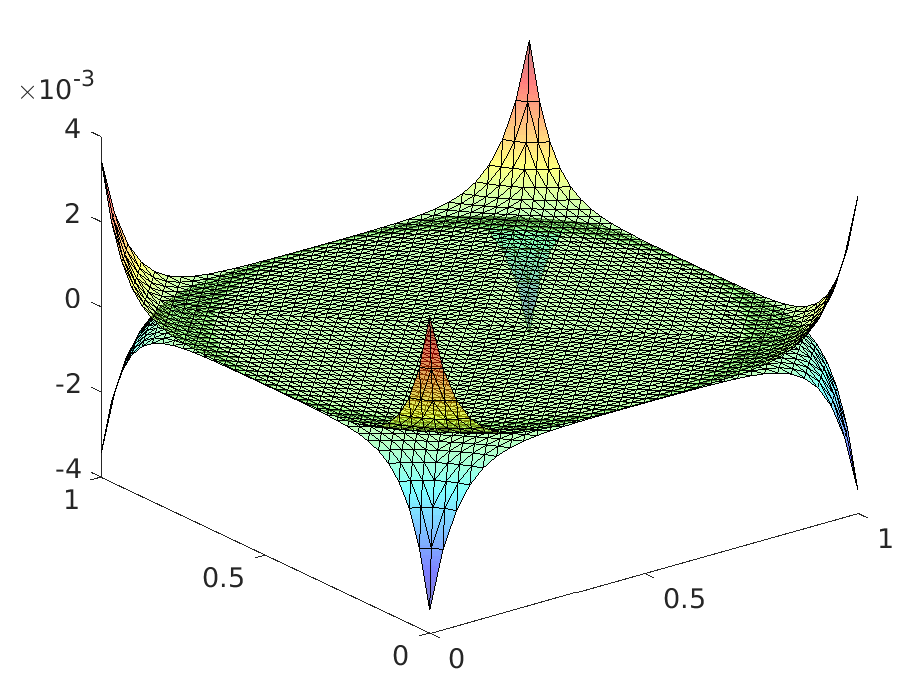
\includegraphics[width=0.48\textwidth]{P2_membrane_cv_J6} \quad
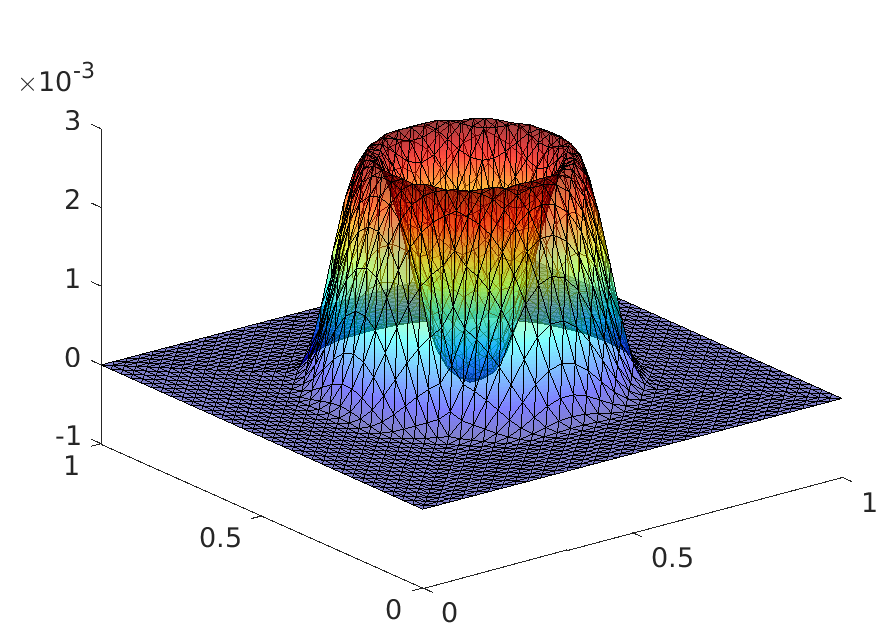
\includegraphics[width=0.48\textwidth]{P2_lambda_cv_J6}
\end{figure}
\end{frame}

\begin{frame}
  \textcolor{red}{\textbf{Number of Newton-min iterations}}
  \vspace*{0.3 cm}
\begin{figure}
\centering
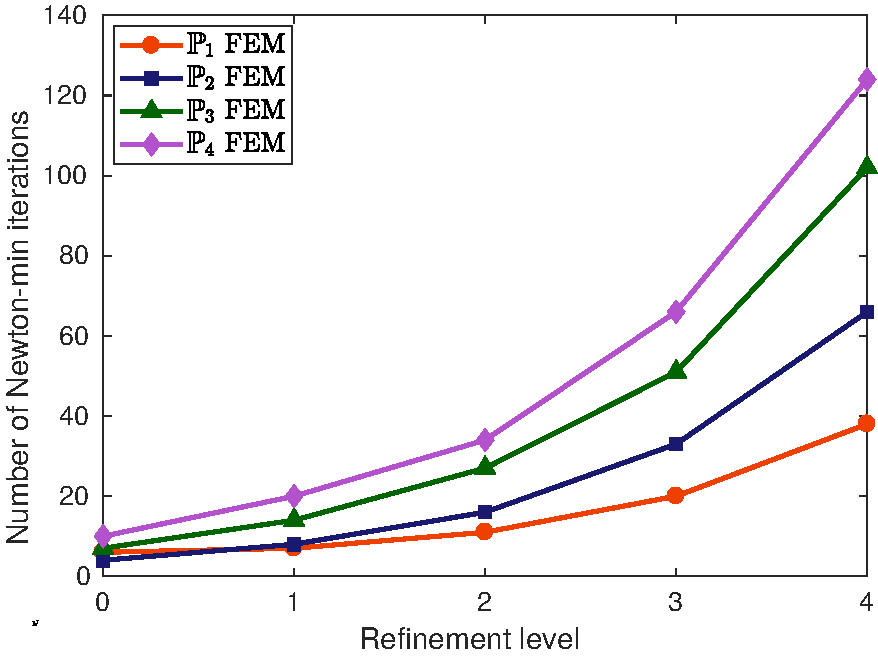
\includegraphics[width=0.48\textwidth]{Number_of_Newton_iter_refinment_level} \quad
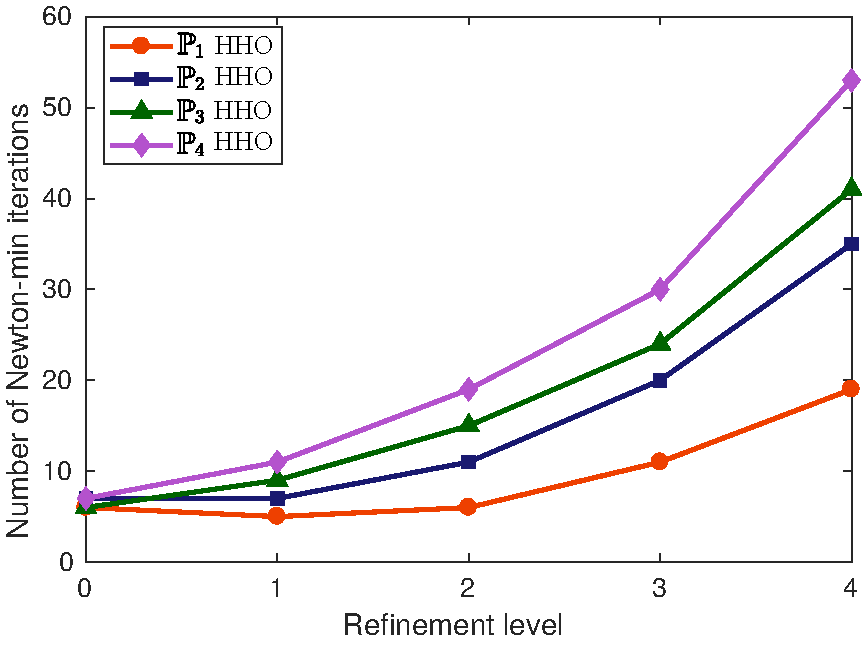
\includegraphics[width=0.48\textwidth]{nb_iter_Newton_HH0}
\end{figure}
  \end{frame}
%%%%%
\begin{frame}
\textcolor{red}{\textbf{Convergence}}
  \begin{figure}
\centering
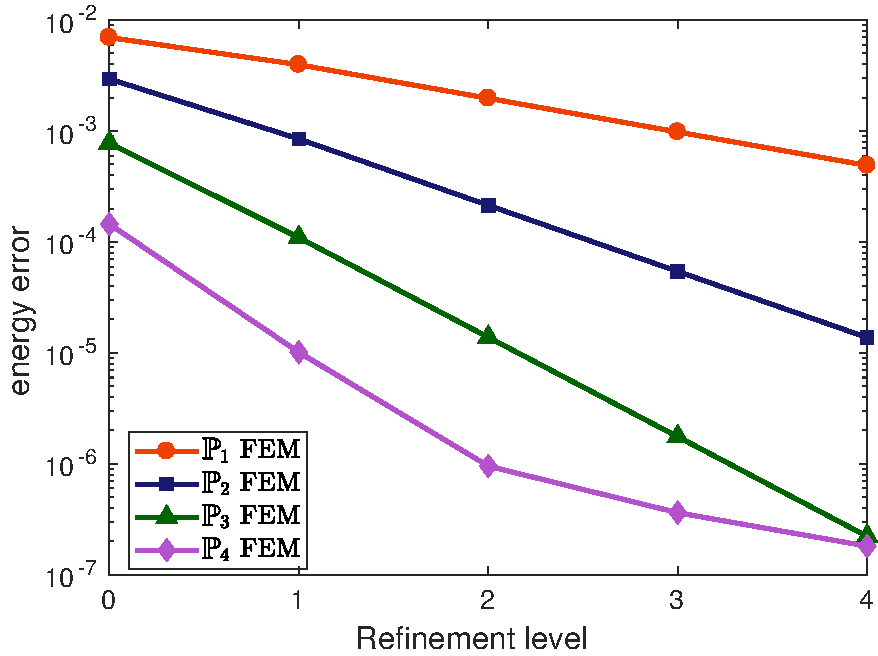
\includegraphics[width=0.48\textwidth]{energy_error_FEM} \quad
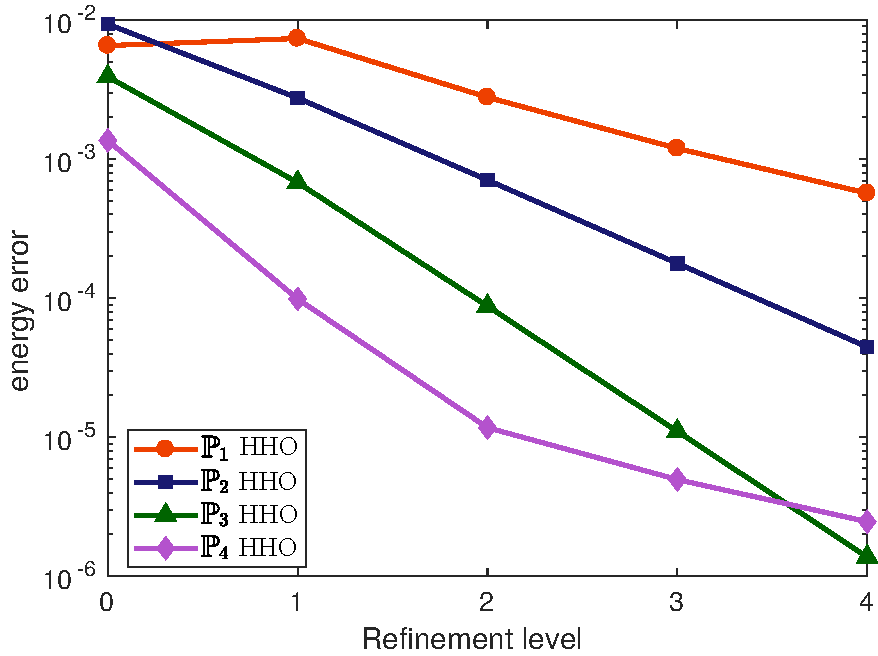
\includegraphics[width=0.48\textwidth]{energy_error_HHO}
\end{figure}
  \end{frame}
\begin{frame}
  \textcolor{cadmiumgreen}{\textbf{A second test case}}
  \begin{align*}
  u_1(r) 
  &\egaldef 
    \begin{cases}
      0 & \text{if } r \leq R ,
      \\
      (r^2 - R^2)^2 &\text{if } r > R ,
    \end{cases}
  %\\
  \quad
  u_2(r) 
  \egaldef 0 ,
\quad
\lambda(r) \egaldef
\begin{cases}
 \dps 1 & \mbox{if } r \leq R,\\
\dps 0 &\mbox{if } r > R,\\
\end{cases}
\end{align*}
This solution is associated to the right-hand sides $f_1$ and $f_2$ given by
\begin{align*}
f_1(r) \egaldef
\begin{cases}
\dps - 8 R^2  &\hspace*{-0.5em}\mbox{if } r \leq R,\\
\dps 8 R^2 - 16 r^2  &\hspace*{-0.5em}\mbox{if } r > R,\\
\end{cases}
\quad
f_2(r) \egaldef
\begin{cases}
\dps 8 R^2 &\hspace*{-0.5em}\mbox{if } r \leq R,\\
\dps 0
&\hspace*{-0.5em}\mbox{if } r > R.\\
\end{cases}
\end{align*}
\vspace*{-0.6 cm}
\begin{figure}
\centering
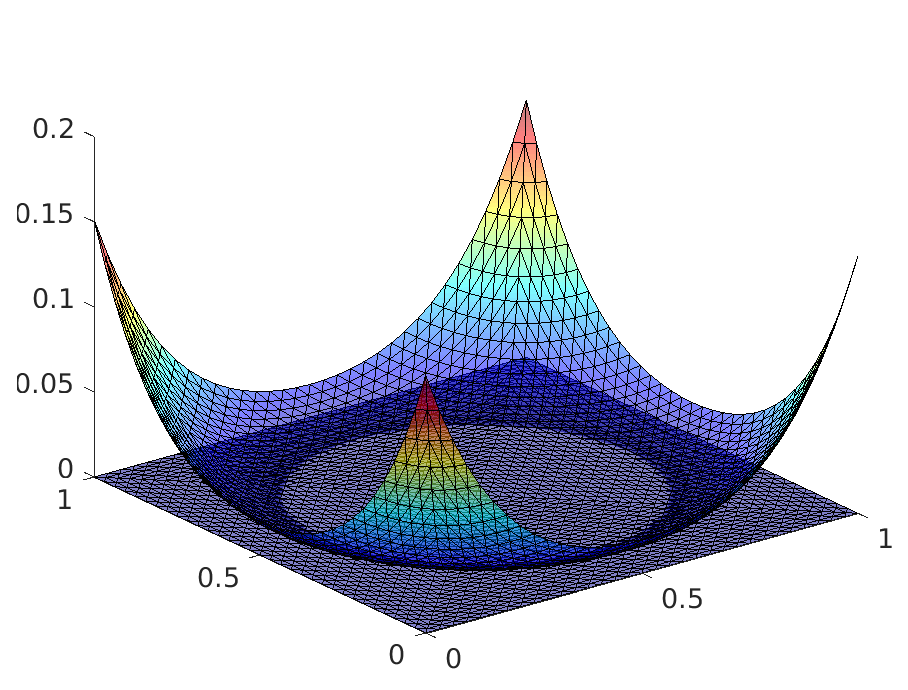
\includegraphics[width=0.40\textwidth]{membrane_P2} \qquad \qquad
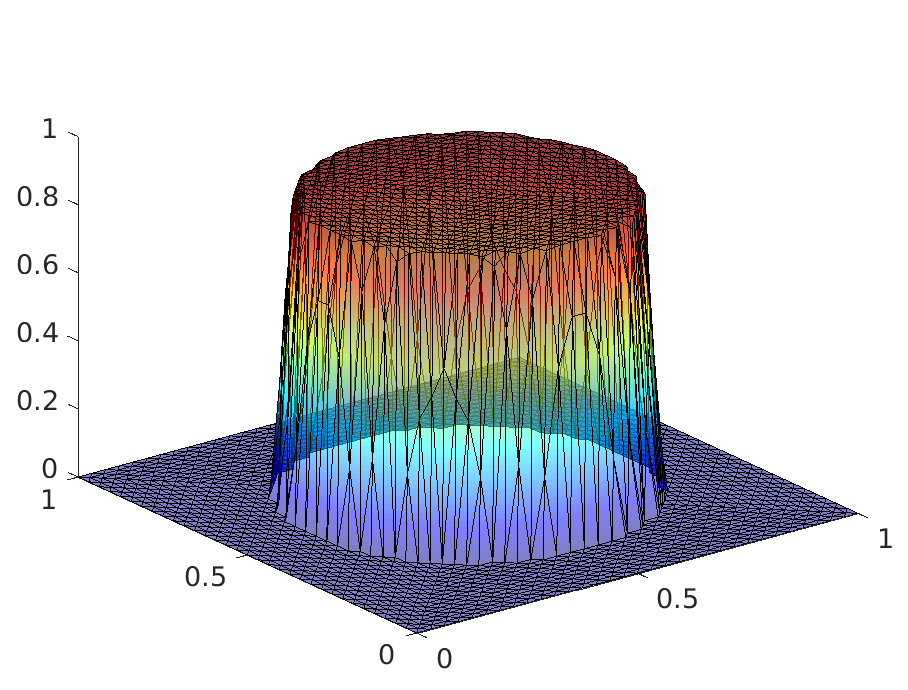
\includegraphics[width=0.40\textwidth]{Lambda_P2}
\end{figure}
\end{frame}

\begin{frame}
  \textcolor{red}{\textbf{Number of Newton-min iterations}}
  \vspace*{0.3 cm}
  \begin{figure}
\centering
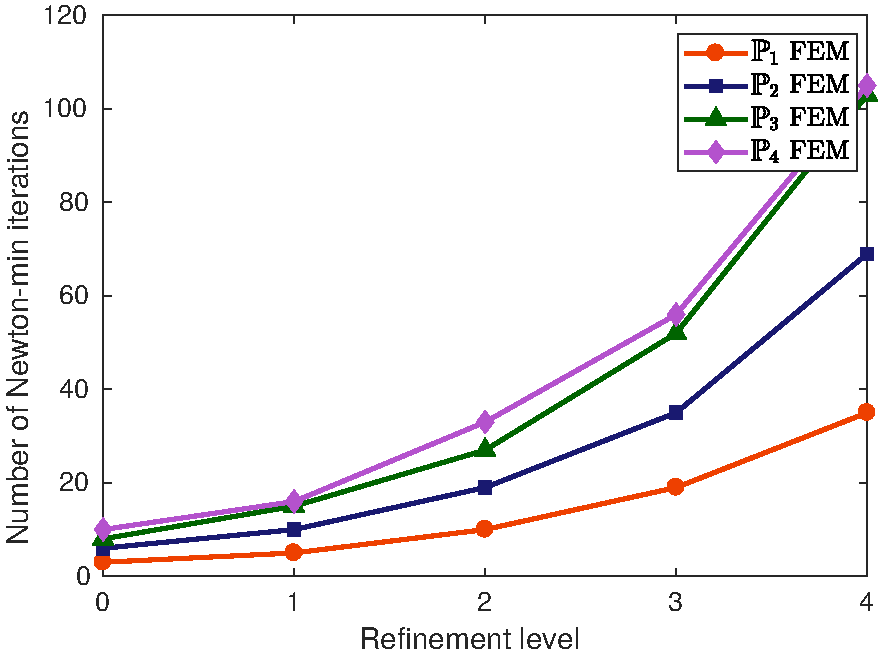
\includegraphics[width=0.48\textwidth]{number_newton_iter_FEM_2nd} \quad
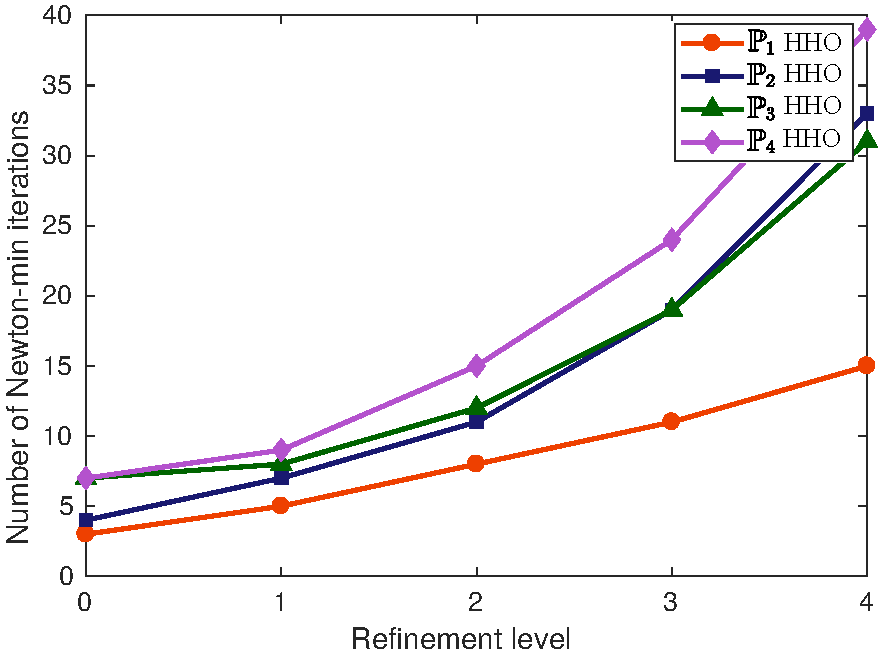
\includegraphics[width=0.48\textwidth]{jump_nb_iter_Newton_HHO}
\end{figure}
  \end{frame}
%%%%%%%%%%%%%%
\begin{frame}
  \textcolor{red}{\textbf{Convergence}}
  \vspace*{0.3 cm}
  \begin{figure}
\centering
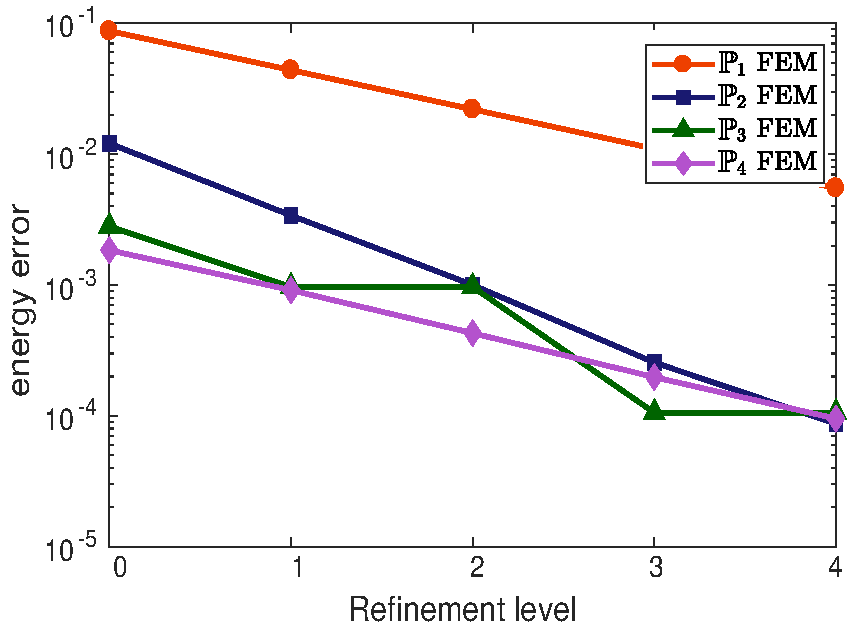
\includegraphics[width=0.48\textwidth]{energy_error_2nd.pdf} \quad
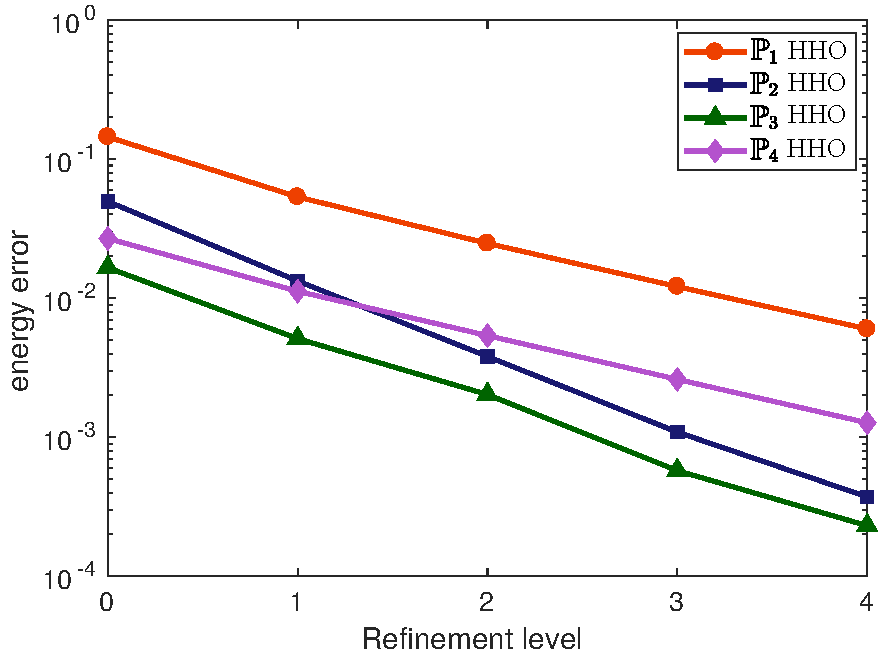
\includegraphics[width=0.48\textwidth]{jump_energy_error_HHO}
  \end{figure}
  \begin{thebibliography}{10}
 \scriptsize{
 \bibitem{Dabaghi:Delay:2020}
 {\sc J.~Dabaghi, G.~Delay}, A unified framework for high-order numerical
discretizations of variational inequalities.
\em{Computers \& Mathematics with Applications} (2021).
}
 \end{thebibliography}
\end{frame}


%%%% CHAP 2

\section{A posteriori analysis}
\subsection{}


\begin{frame}
  %%%%%%%%%%%%%%%%%%%
\frametitle{A posteriori analysis for finite elements}
\begin{equation*}
\tnorm{\bu-\bu_h^{\kk,\ii}}_{\Omega} \egaldef \left(\sum_{\ialf = 1}^2 \mu_\ialf \left\|\nab \left(\uialf-\uialfh^{\kk,\ii} \right)\right\|_{\Omega}^2 \right)^{\frac{1}{2}} \leq \eta^{\kk,\ii} \egaldef \left(\sum_{K \in Th}\left[\eta_{K}(\bu_h^{\kk,\ii}) \right]^2\right)^{\frac{1}{2}}
\end{equation*}
\begin{itemize}
\item $\eta_{K}(\bu_h^{\kk,\ii})$ local estimator depending on the approximate solution 
\item $\eta^{\kk,\ii} \leq \eta_{\mathrm{disc}}^{\kk,\ii} + \eta_{\mathrm{lin}}^{\kk,\ii} + \eta_{\mathrm{alg}}^{\kk,\ii}$: identification of the error components
\item $\eta_{K}(\bu_h^{\kk,\ii}) \leq$ local error + $\underbrace{\mathrm{local \ contact \ term}}_{\mathrm{\textcolor{midnightblue}{typically \ very \ small}}}$: local efficiency
\item adaptive inexact stopping criteria based on the error components
\end{itemize} 
\invisible<1>{
\textcolor{red}{We employ the methodology of equilibrated flux reconstruction to obtain local error estimators.}
\newline 
\footnotesize{Destuynder \& M\'etivet (1999) Braess \& Sch\"oberl (2008), Ern \& Vohral{\'{\i}}k (2013)}
\invisible<2>{
}}
\end{frame}
%
\begin{frame}
\frametitle{Component flux reconstruction}
\textcolor{cadmiumgreen}{\textbf{Motivation:}}
\begin{equation*}
-\mu_\ialf \nab u_{\ialf} \in \HdivOmeg,  \quad  -\mu_\ialf \nab u_{\ialf h}^{\kk,\ii} \not \in \HdivOmeg, \quad \nab {\cdot} \left(-\mu_\ialf \nab u_{\ialf h}^{\kk,\ii} \right) \neq f_\ialf -(-1)^{\ialf} \lambh^{\kk,\ii}
\end{equation*}
\invisible<1>{
\textcolor{cadmiumgreen}{\textbf{Flux reconstruction:}}
\begin{equation*}
{\bm \sigma}_{\ialf h}^{\kk,\ii} \in \HdivOmeg \quad \left(\nab {\cdot} {\bm \sigma}_{\ialf h}^{\kk,\ii}, 1 \right)_K = \left( f_\ialf -(-1)^{\ialf} \lambh^{\kk,\ii}, 1  \right)_K 
\end{equation*}
\invisible<2>{
\textcolor{cadmiumgreen}{\textbf{Decomposition of the flux:}}
\begin{equation*}
{\bm \sigma}_{\ialf h}^{\kk,\ii}  = {\bm \sigma}_{\ialf h, \mathrm{alg}}^{\kk,\ii} + {\bm \sigma}_{\ialf h, \mathrm{disc}}^{\kk,\ii}
\end{equation*}
\invisible<3>{
\textcolor{cadmiumgreen}{\textbf{Algebraic error flux reconstruction:}}
\begin{equation*}
{\bm \sigma}_{\ialf h, \mathrm{alg}}^{\kk,\ii} \in \HdivOmeg \quad \nab {\cdot} {\bm \sigma}_{\ialf h, \mathrm{alg}}^{\kk,\ii}=r_{\ialf h}^{\kk,\ii} \quad \mbox{where} \quad r_{\ialf h}^{\kk,\ii} \quad \mbox{is the functional representation of} \quad {\bm R}_{\ialf h}^{\kk,\ii}
\end{equation*}
\scriptsize{Pape{\v z}, R{\"u}de, Vohral{\'{\i}}k and Wohlmuth (2020).}
\newline
\invisible<4>{
\normalsize{\textcolor{cadmiumgreen}{\textbf{Discretization flux reconstruction:}}
\begin{equation*}
{\bm \sigma}_{\ialf h, \mathrm{disc}}^{\kk,\ii} \in \HdivOmeg \quad \left(\nab {\cdot} {\bm \sigma}_{\ialf h,\mathrm{disc}}^{\kk,\ii}, 1 \right)_K = \left( f_\ialf -(-1)^{\ialf} \lambh^{\kk,\ii} - r_{\ialf h}^{\kk,\ii}, 1  \right)_K
\end{equation*}
}
\invisible<5>{
}}}}}
\end{frame}
%
%%%%ALG FLUX RECONSTRUCTION
% \begin{frame}
% \frametitle{Algebraic flux reconstruction}
% \vspace*{-0.5 cm}
% \begin{equation*}
% \begin{array}{lclcc}
% \left({\bm \sigma}_{\ialf j,\mathrm{alg}}^{\kk,\ii,\ba}, \tauj\right)_{\omajminusun}-\left(\gamma_{\ialf j}^{\kk,\ii,\ba},\nab {\cdot} \tauj\right)_{\omajminusun} &=& 0 & \forall \tauj\in \Vspacejjmuna, \\
% \left(\nab {\cdot} {\bm \sigma}_{\ialf j,\mathrm{alg}}^{\kk,\ii,\ba}, q_{j}\right)_{\omajminusun}&=&\dps\left(\tilde{g}_{\ialf j}^{\kk,\ii,\ba}, q_{j}\right)_{\omajminusun} & \forall q_{j} \in \Qspacejjmuna,
% \end{array}
% \end{equation*}
% \vspace{-0.8 cm}
% \begin{minipage}[c]{.55 \linewidth}
% \vspace{-0.8 cm}
% \begin{equation*}
% \begin{split}
% \Vspacejjmuna &\egaldef \left\{ \tauj \in \RTp(\omajminusun),
% \ \tauj {\cdot} \nnomajminusun =0 \mbox{ on } \partial \omajminusun \right\}, \\
% \Qspacejjmuna &\egaldef \Pp^{0}({\omajminusun}), \ \ba \in \mathcal{V}_{j-1}^{\mathrm{int}}
% \end{split}
% \end{equation*}
% \vspace{-0.2 cm}
% \invisible<1-2>{
% \begin{equation*}
% \begin{split}
% \Vspacejjmuna & \egaldef\left\{ \tauj \in \RTp(\omajminusun),
% \ \tauj {\cdot} \nnomajminusun=0 \  \mbox{on} \ \partial \omajminusun \backslash \partial \Omega\right\},
% \\
% \Qspacejjmuna & \egaldef \Pp({\omajminusun}), \ \ba \in \mathcal{V}_{j-1}^{\mathrm{ext}}
% \end{split}
% \end{equation*}
% }
% \end{minipage}
% \hfill
% \begin{minipage}[c]{.42 \linewidth}
% \hspace{3 cm}
% \begin{figure}
%   \begin{overprint}
%     \onslide<1>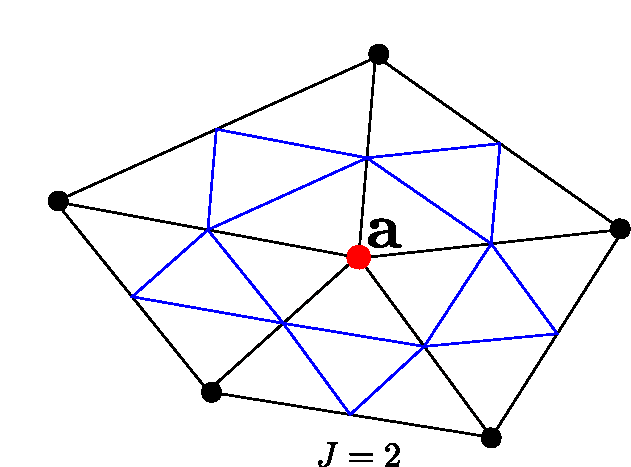
\includegraphics[width=0.9 \textwidth]{patch_alg_1.pdf}
%     \onslide<2>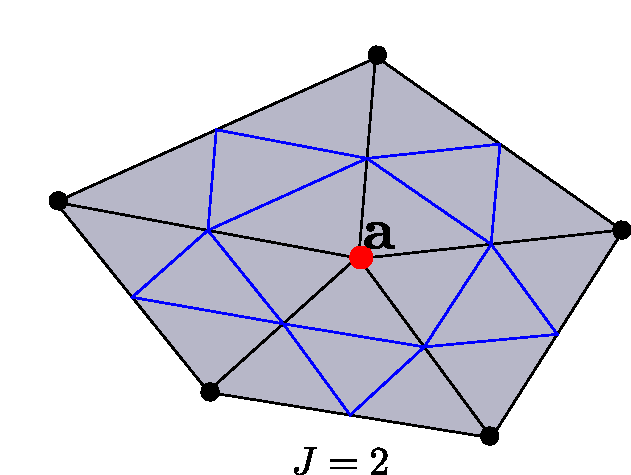
\includegraphics[width=0.9 \textwidth]{patch_alg_2.pdf}
%     \onslide<3>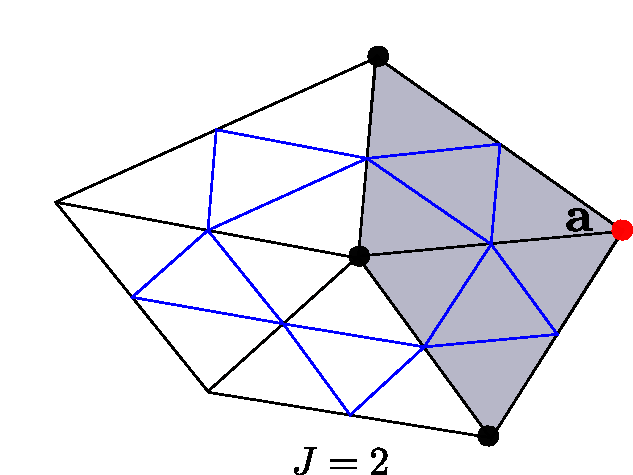
\includegraphics[width=0.9 \textwidth]{patch_alg_2_bis.pdf}
%     \onslide<4>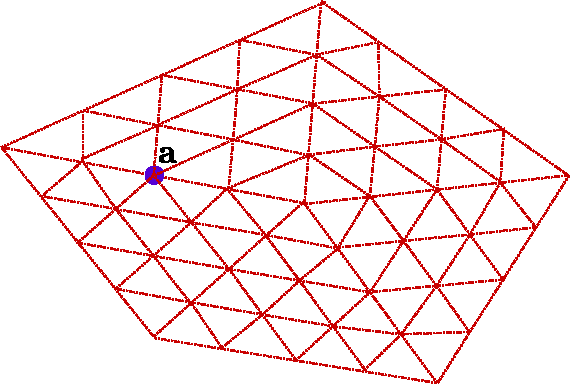
\includegraphics[width=0.9 \textwidth]{patch_alg_3.pdf}
%     \onslide<5->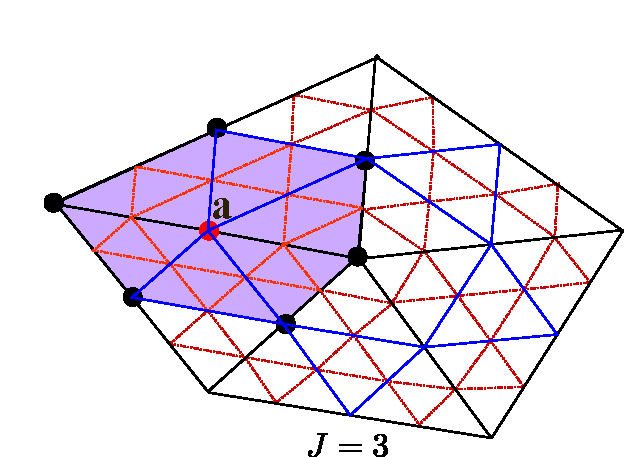
\includegraphics[width=0.9 \textwidth]{patch_alg_4.pdf} 
%     \end{overprint}
% \end{figure}
% \end{minipage}
% \vspace{-0.2 cm}
% \invisible<1-4>{
% \begin{equation*}
% {\bm \sigma}_{\ialf j,\mathrm{alg}}^{\kk,\ii} \egaldef \sum_{j=1}^{J} \sum_{\ba \in \mathcal{V}_{j-1}} {\bm \sigma}_{\ialf j,\mathrm{alg}}^{\kk,\ii,\ba}
% \end{equation*}
% }
% \end{frame}
%
%
\begin{frame}
\frametitle{Estimators}

\textcolor{cadmiumgreen}{\textbf{Violations of physical properties of the numerical solution}}
\begin{equation*}
{\bm \sigma}_{\ialf h}^{\kk,\ii} \neq -\nab \uialfh^{\kk,\ii}, \qquad \nab {\cdot} {\bm \sigma}_{\ialf h}^{\kk,\ii} \neq f_\ialf -(-1)^{\ialf} \lambh^{\kk,\ii}
\end{equation*}
\invisible<1>{
\textcolor{midnightblue}{\textbf{Flux estimator:}}
\begin{equation*}
\eta_{\mathrm{F},K,\ialf}^{\kk,\ii} \egaldef \left\|\mu_\ialf^{\frac{1}{2}} \nab u_{\ialf h}^{\kk,\ii}
+\mu_\ialf^{-\frac{1}{2}} {\bm \sigma}_{\ialf h}^{\kk,\ii}\right\|_{K},
\end{equation*}
\textcolor{midnightblue}{\textbf{Residual estimator:}}
\begin{equation*}
\eta_{\mathrm{R},K,\ialf}^{\kk,\ii} \egaldef \frac{h_K}{\pi} \mu_\ialf^{-\frac{1}{2}}
\left\|f_\ialf - \nab {\cdot} {\bm \sigma}_{\ialf h}^{\kk,\ii} -(-1)^{\ialf} \lambh^{\kk,\ii} \right\|_{K},
\end{equation*}
\invisible<2>{
}}
\end{frame}
%
\begin{frame}
\textcolor{cadmiumgreen}{ \textbf{Violations of the complementarity constraints}}\\
\invisible<1>{
\textcolor{red}{p = 1:} \ \textcolor{midnightblue}{\textbf{at convergence:}} 
\vspace{-0.1 cm}
\begin{equation*} 
(\uunh \hspace{-0.05 cm} - \hspace{-0.05 cm} \udeuxh)(\ba) \hspace{-0.05 cm} \geq \hspace{-0.05 cm} 0 \hspace{-0.05 cm} \Rightarrow \hspace{-0.05 cm} \uh \hspace{-0.05 cm} \in \hspace{-0.05 cm} \Kg, \hspace{0.1 cm} \lambh(\ba) \hspace{-0.05 cm} \geq \hspace{-0.05 cm} 0 \hspace{-0.05 cm} \Rightarrow \hspace{-0.05 cm} \lambh \hspace{-0.05 cm} \in \hspace{-0.05 cm} \Lambda, \hspace{0.1 cm} \lambh(\ba) \hspace{-0.05 cm} \cdot \hspace{-0.05 cm} (\uunh \hspace{-0.05 cm} - \hspace{-0.05 cm} \udeuxh)(\ba) \hspace{-0.05 cm} = \hspace{-0.05 cm} 0 \textcolor{red}{\bm{\not \Rightarrow}} \lambh \hspace{-0.05 cm} \cdot \hspace{-0.05 cm} (\uunh \hspace{-0.05 cm} - \hspace{-0.05 cm} \udeuxh) \hspace{-0.05 cm} = \hspace{-0.05 cm} 0
\end{equation*}
\invisible<2>{
\textcolor{red}{p = 1:} \ \textcolor{midnightblue}{\textbf{at each inexact semismooth step:}}
\begin{equation*}
(\uunh^{\kk,\ii}-\udeuxh^{\kk,\ii})(\ba) \not \geq 0 \quad \lambh^{\kk,\ii}(\ba) \not \geq 0 \quad \lambh^{\kk,\ii}(\ba) \cdot (\uunh^{\kk,\ii}-\udeuxh^{\kk,\ii})(\ba)\not=0 \quad \forall \ba \in \Vhint
\end{equation*}
\invisible<3>{
\textcolor{red}{$p \geq 2$:} \ \textcolor{midnightblue}{\textbf{at convergence:}} 
\vspace{-0.1 cm}
\begin{equation*}
(\uunh - \udeuxh)(\bx_l) \geq 0 \ \textcolor{red}{\bm{\not \Rightarrow}} \ \uh \in \Kg \ , \ \left(\lambh,\psihl \right)_{\Omega} \geq 0 \ \textcolor{red}{\bm{\not \Rightarrow}} \ \lambh \in \Lambda  
\end{equation*}
\begin{equation*}
\left(\lambh,\uunh-\udeuxh\right)_{\Omega} = 0 \ \textcolor{red}{\bm{\not \Rightarrow}} \ \lambh \cdot \left(\uunh-\udeuxh\right) = 0
\end{equation*}
\invisible<4>{
\textcolor{red}{$p \geq 2$:} \ \textcolor{midnightblue}{\textbf{at each inexact semismooth step:}}
\begin{equation*}
(\uunh^{\kk,\ii} - \udeuxh^{\kk,\ii})(\bx_l) \not \geq 0 \ , \ \left(\lambh^{\kk,\ii},\psihl \right)_{\Omega} \not \geq 0 \ \forall \bx_l \in \Vdpint \ \left(\lambh^{\kk,\ii},\uunh^{\kk,\ii}-\udeuxh^{\kk,\ii}\right)_{\Omega} \neq 0
\end{equation*}
\invisible<5>{
\textcolor{midnightblue}{\textbf{Contact estimator:}}
\begin{equation*}
\eta_{\mathrm{C},K}^{\kk,\ii} \egaldef 2 \left(\lambh^{\kk,\ii,\mathrm{pos}},\uunh^{\kk,\ii}-\udeuxh^{\kk,\ii} \right)_K,
\end{equation*}
\invisible<6>{
\textcolor{midnightblue}{\textbf{Nonconformity estimators:}}  We construct $\textcolor{electricpurple}{\Ktildeghp} \subset \Kg$, $\lambh^{\kk,\ii} \hspace{-0.05 cm}= \hspace{-0.05 cm} \lambh^{\kk,\ii,\mathrm{pos}} \hspace{-0.1 cm} + \hspace{-0.1 cm} \lambh^{\kk,\ii,\mathrm{neg}}$ $\Rightarrow$ 3 estimators.
\invisible<7>{
}}}}}}}
\end{frame}
%
\begin{frame}
\begin{theorem}[A posteriori error estimate]
\begin{equation*}
\tnorm{\bu-\uh^{\kk,\ii}} \leq \hspace{-0.1 cm}
\left\{ \left(\left(\sum_{K \in \Th} \sum_{\ialf = 1}^2
\left(\eta_{\mathrm{F},K,\ialf}^{\kk,\ii} \hspace{-0.1 cm}+\hspace{-0.05 cm} \eta_{\mathrm{R},K,\ialf}^{\kk,\ii} \right)^2 \right)^{\frac{1}{2}} \hspace{-0.1 cm}+ \hspace{-0.05 cm}\eta_{\mathrm{nonc},1}^{\kk,\ii} + \eta_{\mathrm{nonc},2}^{\kk,\ii} \right)^2
\hspace{-0.1 cm}+ \hspace{-0.05 cm} \eta_{\mathrm{nonc},3}^{\kk,\ii} + \hspace{-0.1 cm}\sum_{K\in\Th} \hspace{-0.1 cm} \eta_{\mathrm{C},K}^{\kk,\ii,\mathrm{pos}} \right\}^{\frac{1}{2}}
\end{equation*}
\end{theorem}
\vspace{-0.1 cm}
\invisible<1>{
\begin{corollary}[Distinction of the error components]
\begin{equation*}
\tnorm{\bu-\uh^{\kk,\ii}} \leq \eta_{\mathrm{disc}}^{\kk,\ii} + \eta_{\mathrm{lin}}^{\kk,\ii} + \eta_{\mathrm{alg}}^{\kk,\ii}
\end{equation*}
\end{corollary}
\invisible<2>{
\begin{minipage}[c]{.32 \textwidth}
\textcolor{red}{\textbf{Adaptive algorithm}}
\\
 \textbf{If} \fcolorbox{violet}{white}{$\eta_{\mathrm{alg}}^{\kk,\ii} \leq \gamma_{\mathrm{alg}} \max  \left\{{\eta_{\mathrm{disc}}^{\kk,\ii}, \eta_{\mathrm{lin}}^{\kk,\ii}}\right\}$} \\
 \qquad  \textbf{Stop linear solver}	
\\
  \textbf{If} \fcolorbox{violet}{white}{ $\eta_{\mathrm{lin}}^{\kk,\ii} \leq \gamma_{\mathrm{lin}} \eta_{\mathrm{disc}}^{n,\kk,\ii}$}
\\
 \qquad {\textbf{Stop nonlinear solver}}
\end{minipage}
\hfill
\invisible<3>{
\begin{minipage}[c]{0.65 \textwidth}
\begin{theorem}[\footnotesize{Local efficiency under adaptive stopping criteria} : \textcolor{red}{p=1}]
\vspace{-0.5 cm}
\begin{equation*}
\begin{split}
\eta_{\mathrm{disc},K}^{\kk,\ii}  \lesssim \hspace{-0.1 cm}  \hspace{-0.1 cm} & \sum_{\ba \in \Vh} \left(\left\| \nab \left(\uialf \hspace{-0.1 cm} - \hspace{-0.1 cm} \uialfh^{\kk,\ii} \right)  \right\|_{\omah} \hspace{-0.15 cm} + \hspace{-0.1 cm} \tnorm{\lambda \hspace{-0.1 cm} - \hspace{-0.1 cm} \lambda_h^{\kk,\ii}(\ba)}_{H^{-1}_{*}(\omah)}\right) \\
& +  \mathrm{contact \ term}
\end{split}
\end{equation*}
\end{theorem}
\end{minipage}
 \invisible<4>{
}}}}
\end{frame}
%
\begin{frame}[noframenumbering]
\centering
\Huge{\textcolor{carmine}{Numerical experiments}}
\end{frame}
%
\begin{frame}
\frametitle{Numerical experiments $\mathbb{P}_2$}

\begin{itemize}
\item 
semismooth solver: \textcolor{blue}{Newton-min}. Linear solver: \textcolor{red}{GMRES} with ILU preconditionner.
\end{itemize}


\begin{figure}
\begin{minipage}[c]{.333\linewidth}
   \centering
   \quad \small{Exact Newton} \scriptsize{\hspace{3 cm} (\textcolor{midnightblue}{$\left\|\bR_{\mathrm{rel,alg}}^{\kk,\ii}\right\| \leq 10^{-12}$, $\left\|\bR_{\mathrm{rel,lin}}^{\kk,\ii}\right\| \leq 10^{-10}$})}
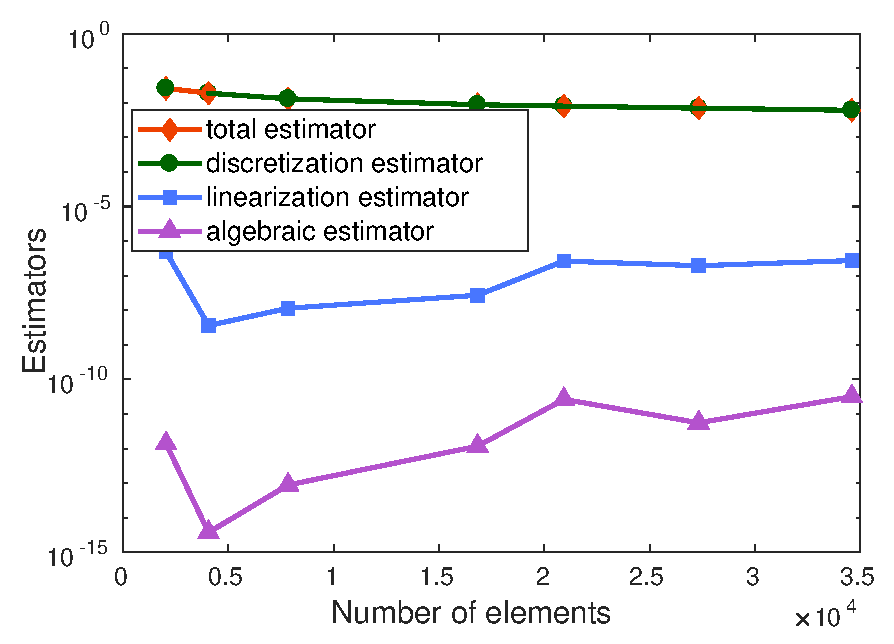
\includegraphics[width=\textwidth]{fig_article_chap_1/exact_resolution_convergence_estimator_number_elements.eps}    \end{minipage}\hfill
\begin{minipage}[c]{.333\linewidth}
   \centering
   \quad \small{Inexact Newton} \hspace{3 cm} \scriptsize{(\textcolor{midnightblue}{$\left\|\bR_{\mathrm{rel,alg}}^{\kk,\ii}\right\| \leq \left\|\bR_{\mathrm{rel,lin}}^{\kk,\ii}\right\|$, $\left\|\bR_{\mathrm{rel,lin}}^{\kk,\ii}\right\| \leq 10^{-10}$})}
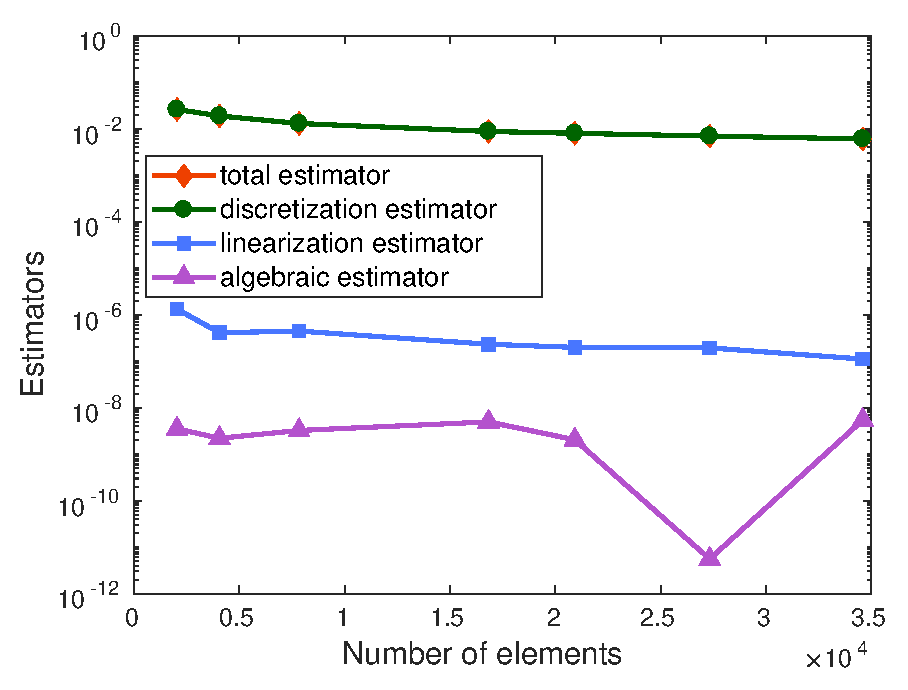
\includegraphics[width=\textwidth]{fig_article_chap_1/inexact_resolution_convergence_estimator_number_elements.eps}    

\end{minipage}\hfill
\begin{minipage}[c]{.33\linewidth}
   \centering
   \small{\small{Adaptive Inexact Newton} \hspace{3 cm} \scriptsize{\textcolor{midnightblue}{($\gammalin=10^{-1}$, $\gammaalg=10^{-1}$)}}}
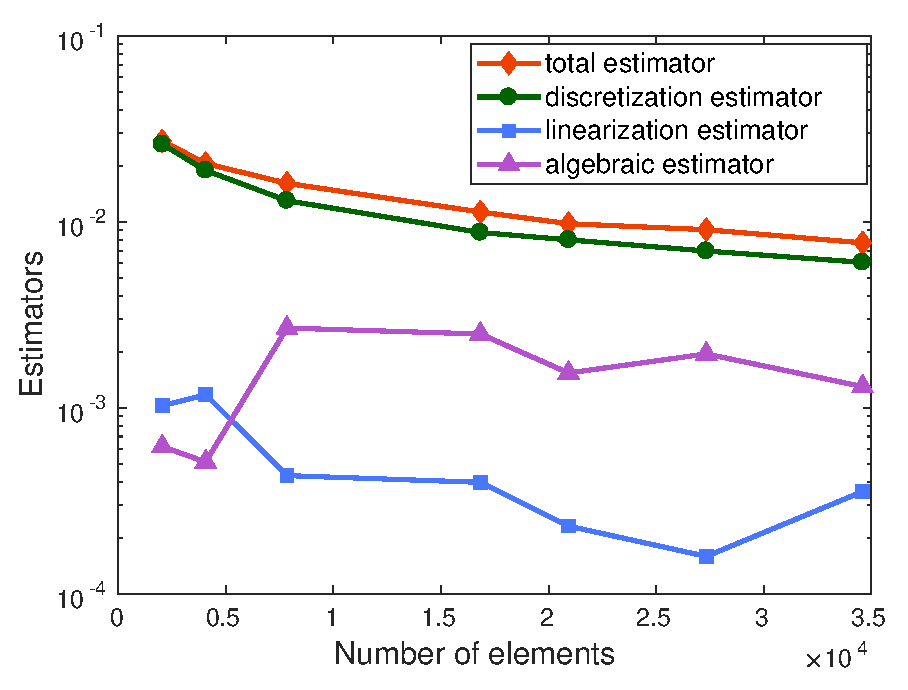
\includegraphics[width=\textwidth]{fig_article_chap_1/adapt_inexact_resolution_convergence_estimator_number_elements.eps}     
\end{minipage}
%\caption{Exact Newton(left), Inexact Newton(middle), adaptive inexact Newton(right)}
\end{figure}

\textcolor{red}{\textbf{Precision is preserved for adaptive inexact semismooth Newton method.}}


\end{frame}

\begin{frame}
\frametitle{Adaptivity}
\hspace{5.5 cm} Exact Newton/Adaptive inexact Newton \hspace{3.5 cm } 
%Inexact Newton
\begin{figure}
   \centering
%% 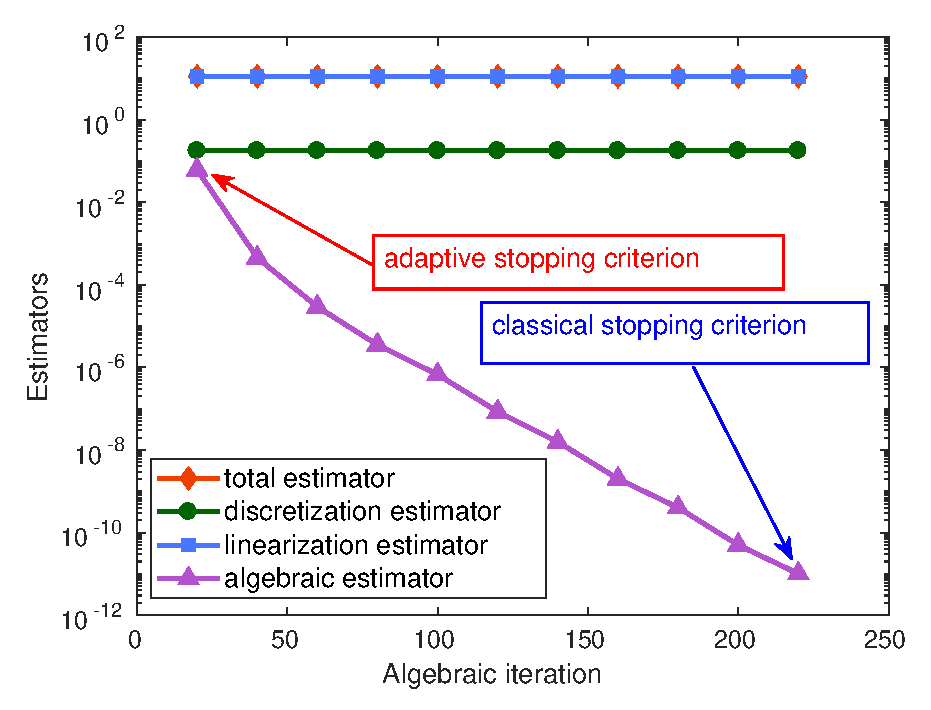
\includegraphics[width=0.50\textwidth]{fig_article_chap_1/exact_adapt_res_estimators_gmres_iter_first_newton_iter_Hmax_015.eps}    
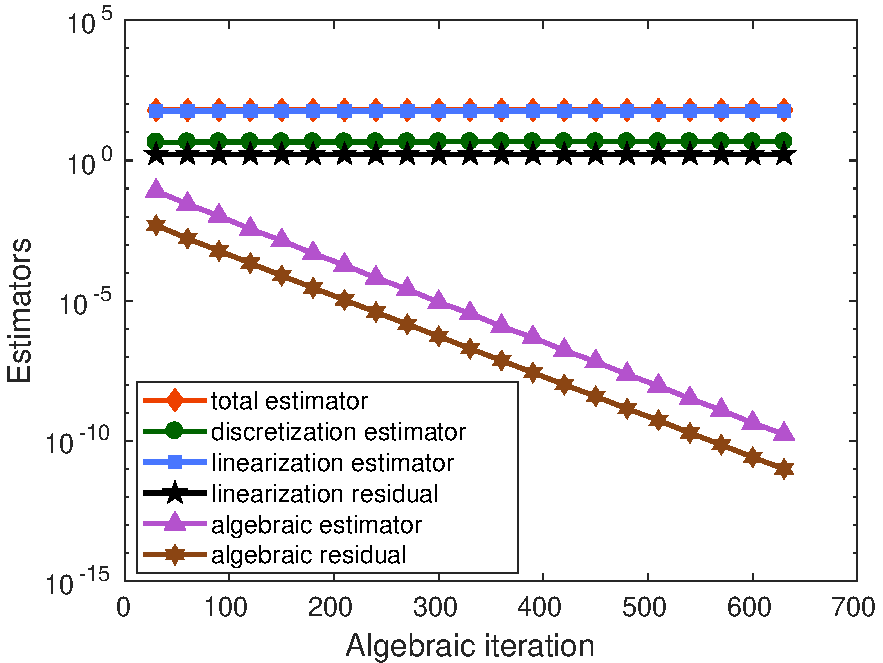
\includegraphics[width=0.50\textwidth]{p2/Exact_P2_estimator_GMRES_per_1stNewton}
%% 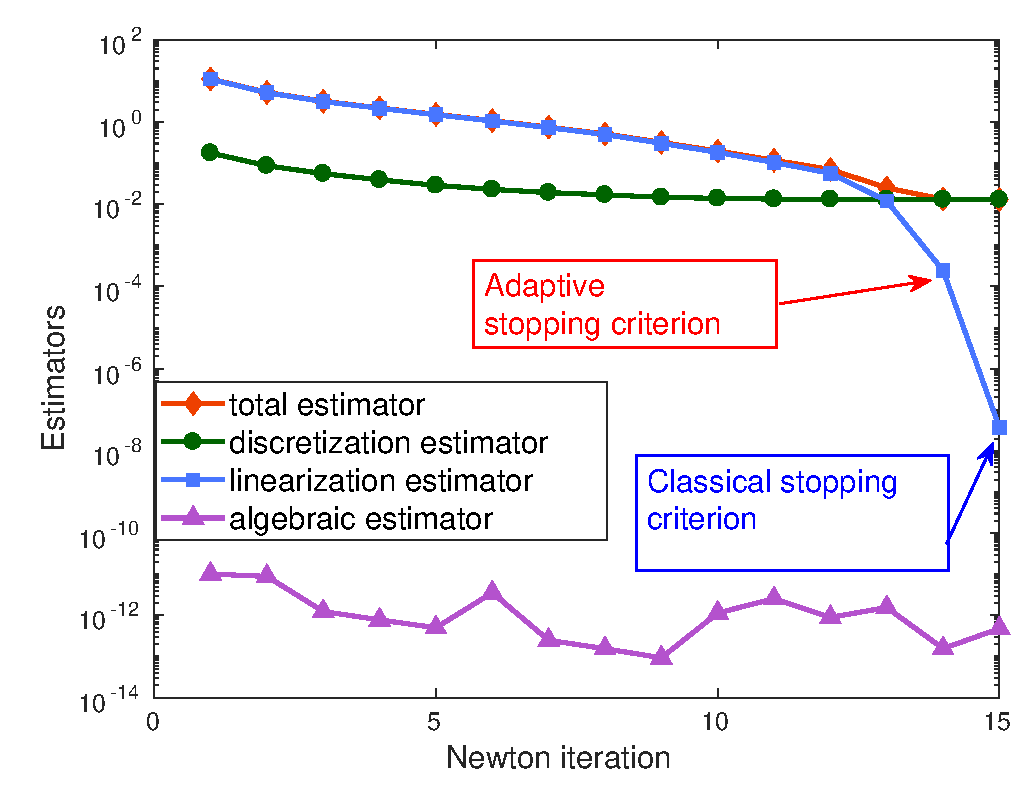
\includegraphics[width=0.49\textwidth]{fig_article_chap_1/exact_adapt_resolution_estimators_newton_iter_Hmax_015.eps}
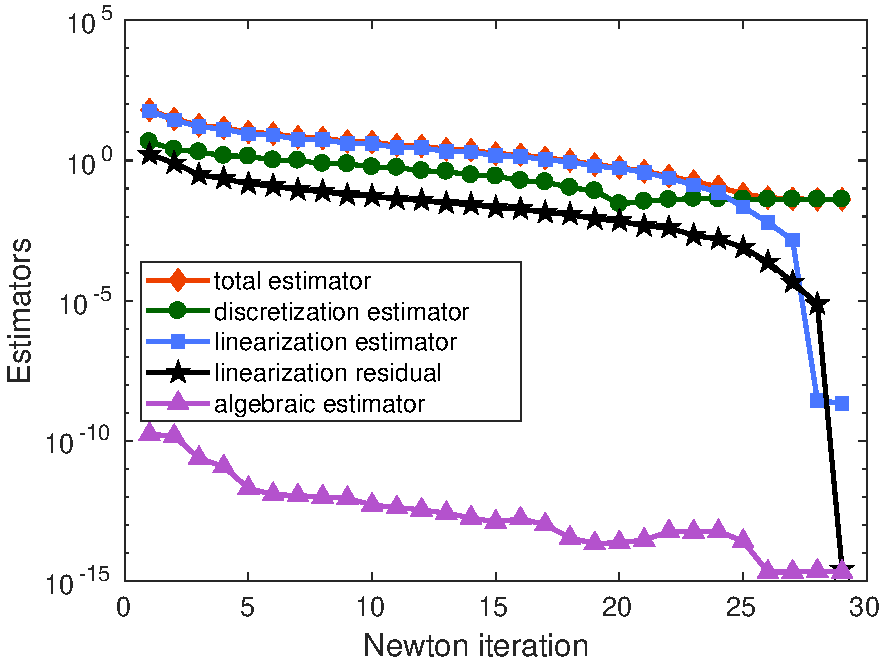
\includegraphics[width=0.49\textwidth]{p2/Exact_P2_estimator_Newton_iter}
\end{figure}
\end{frame}

\begin{frame}
\frametitle{Overall performance}
\begin{figure}
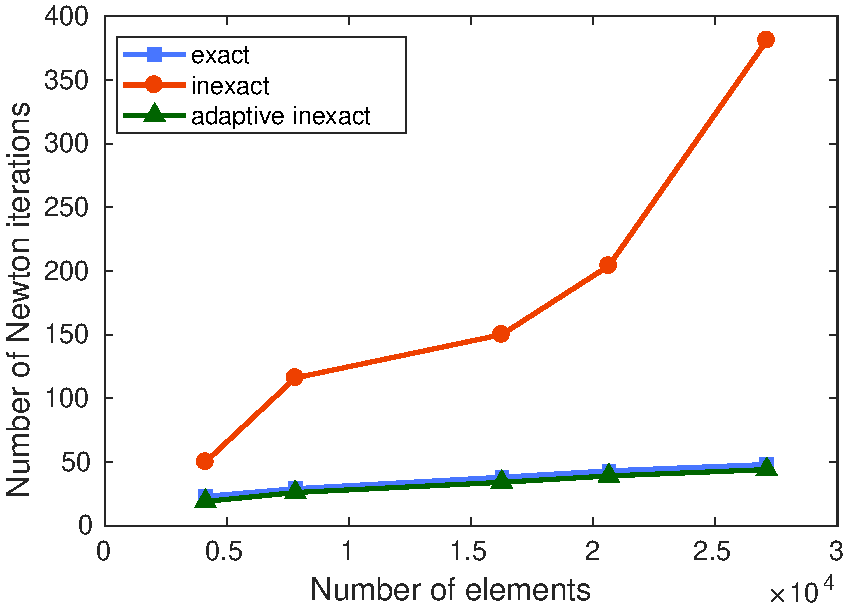
\includegraphics[width=0.5\textwidth]{p2/P2_number_Newton_iter_per_elements}  
%% 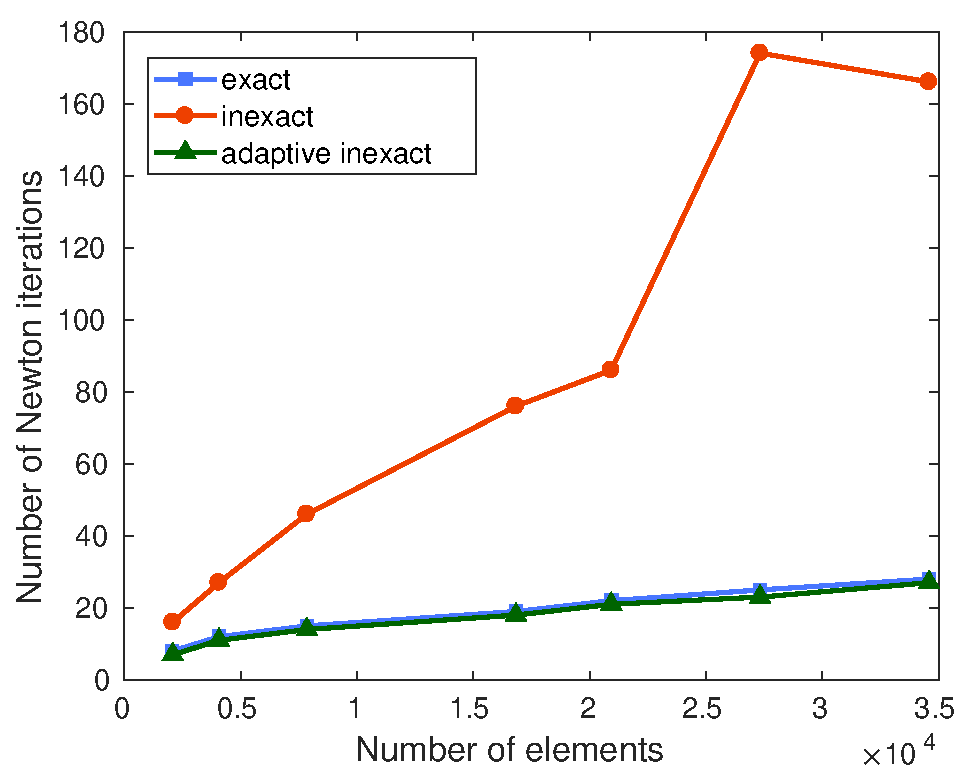
\includegraphics[width=0.46\textwidth]{fig_article_chap_1/comparison_three_methods_number_Newton_iter_number_elements.eps}
\quad  
%% 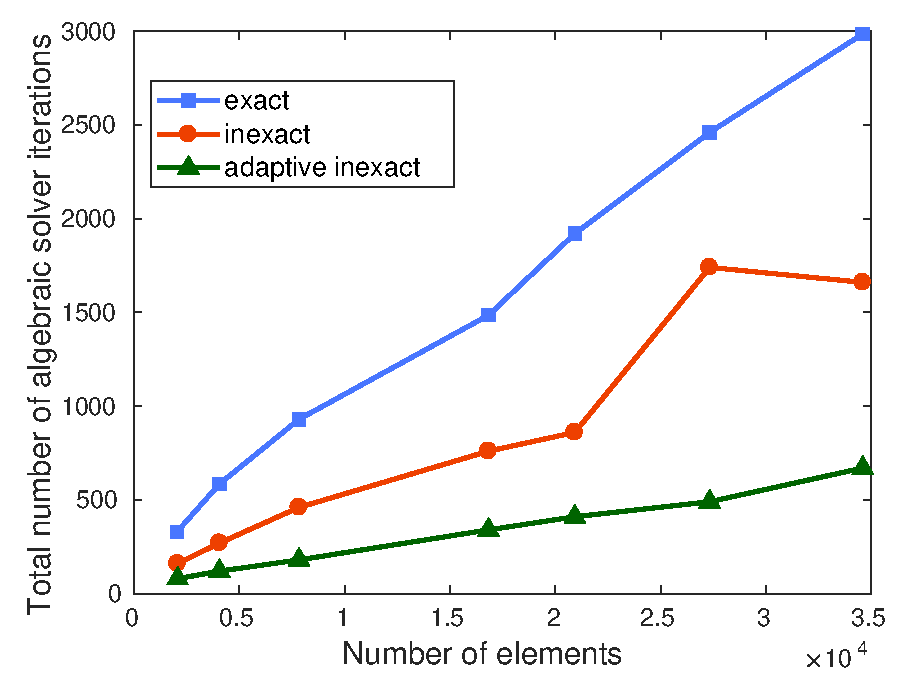
\includegraphics[width=0.49\textwidth]{fig_article_chap_1/comparison_three_methods_total_number_Newton_Gmres_iter_number_elements.eps}
 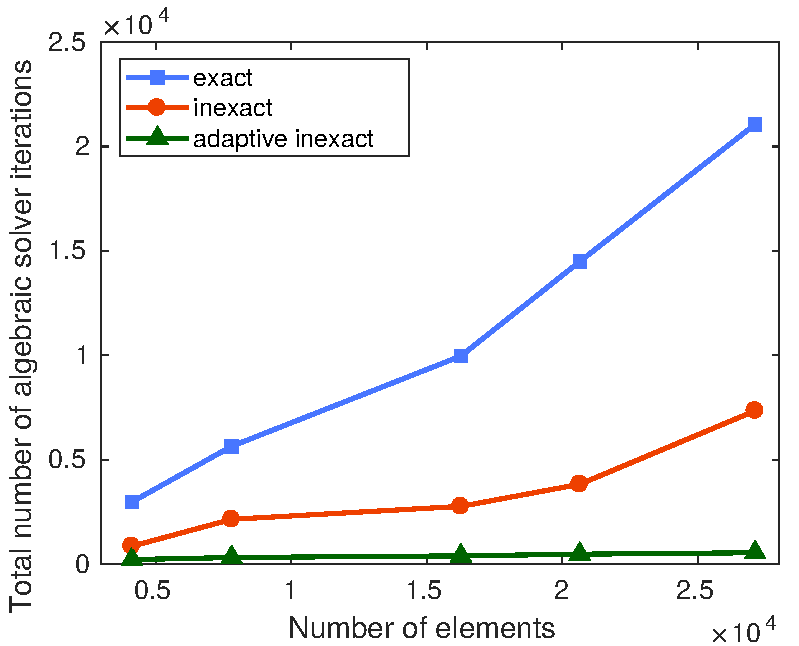
\includegraphics[width=0.46\textwidth]{p2/P2_tot_number_GMRES_iter_per_elements}
\end{figure}
\end{frame}
%%%%
\begin{frame}
  \vspace*{0.1 cm}
  \hspace{0.5 cm}\textcolor{red}{\textbf{Effectivity indices:}} $\mathrm{I}_{\mathrm{eff}} \egaldef \frac{\eta^{\kk,\ii}}{\tnorm{\bu-\bu_h^{\kk,\ii}}_{\Omega}}$ \hspace{3 cm} \textcolor{red}{\textbf{contact estimator}}
\vspace*{-0.2 cm}
  \begin{figure}
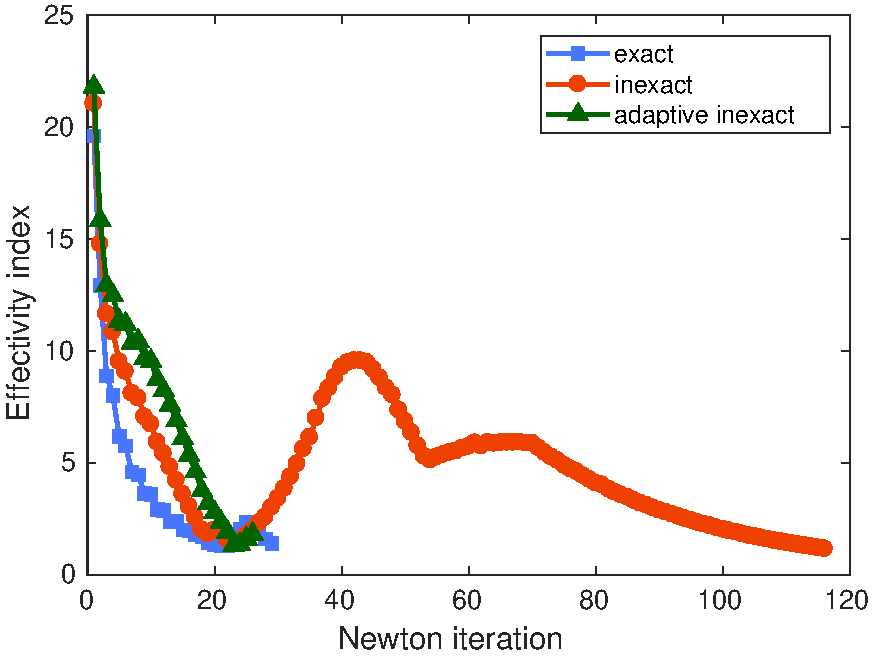
\includegraphics[width=0.46 \textwidth]{p2/P2_effectivity_index_three_methods}    
%% 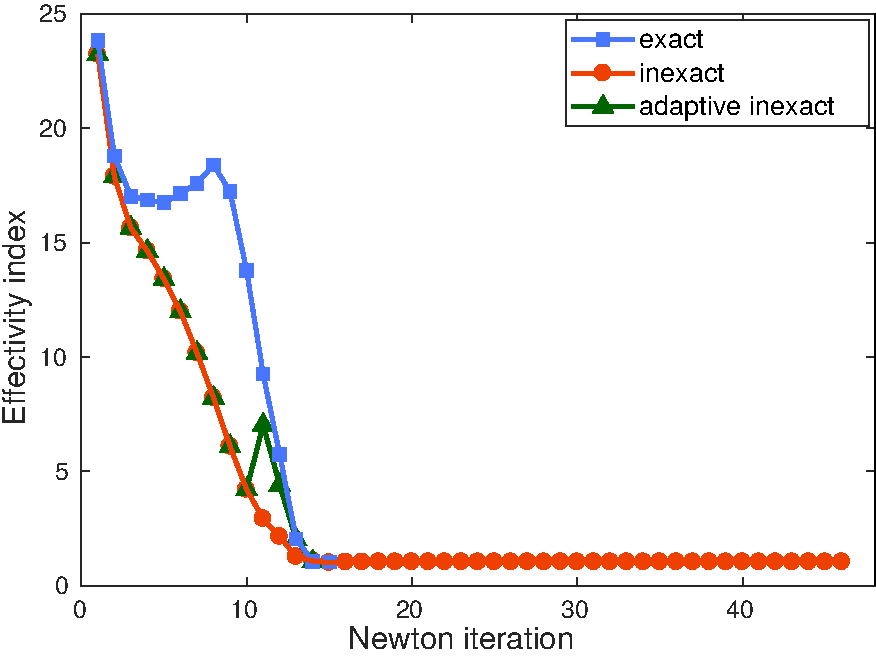
\includegraphics[width=0.46 \textwidth]{fig_article_chap_1/effectivity_index_3_methods_Hmax_015.pdf}
\quad 
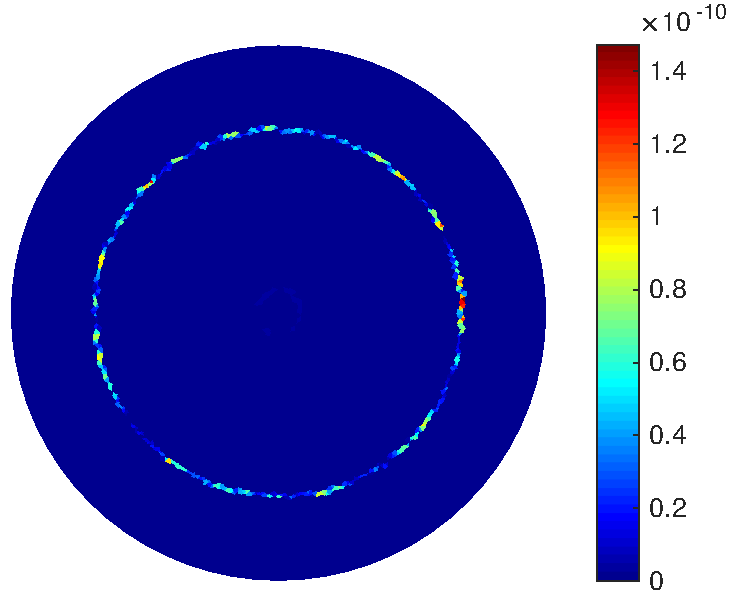
\includegraphics[width=0.49 \textwidth]{fig_article_chap_1/modif_fig_contact_estimator_hmax0,09_Dt0,001_tt180}
\end{figure}
\begin{thebibliography}{10}
 \scriptsize{
 \bibitem{Dabaghi:Martin:Vohralik:2020}
 {\sc J.~Dabaghi, V.~Martin, M.~Vohral\'{i}k}, Adaptive Inexact Semismooth Newton Methods for the
Contact Problem Between Two Membranes.
\em{Journal of Scientific Computing} (2020).
}
 \end{thebibliography}
\end{frame}

%%%%%%%%%%% CHAP 3

\section{Extension to unsteady problems}
\subsection{}

%%%% Part 3



\begin{frame}
\frametitle{ Parabolic model problem with linear complementarity constraints}
\begin{equation*}
\dps \left\lbrace\begin{array}{llccc} 
\dps \textcolor{red}{\partial_t u_1} -\mu_1 \Delta u_1-\lambda =
f_1 \qquad \hspace{5.75 cm}\mbox{in} \ \quad \Omega \times \left]0,T\right[, \\ 
\dps \dps \textcolor{red}{\partial_t u_2} -\mu_2 \Delta u_2+\lambda =
f_2 \qquad \hspace{5.75 cm} \mbox{in} \ \quad \Omega \times \left]0,T\right[,\\ 
\textcolor{electricpurple}{u_1-u_2} \geq 0, \quad \textcolor{carmine}{\lambda} \geq 0, \quad \dps \textcolor{carmine}{\lambda} (\textcolor{electricpurple}{u_1-u_2}) =0 \hspace{3.8 cm}\mbox{in} \quad \
\Omega \times \left]0,T\right[,\\ 
\dps u_1=g_1 \qquad \hspace{8.3 cm} \mbox{on} \hspace{0.35 cm} \partial \Omega \times \left]0,T\right[,\\ 
\dps
u_2=g_2 \qquad \hspace{8.32 cm} \mbox{on} \hspace{0.32 cm} \partial \Omega \times \left]0,T\right[,\\
u_1(\bx,0) = u_1^0(\bx), \ u_2(\bx,0) = u_2^0(\bx), \ u_1^0(\bx)-u_2^0(\bx) \geq 0 \hspace{1.1 cm} \mbox{in}  \hspace{0.44 cm} \Omega.
\end{array}
\right.
\end{equation*}
\invisible<1>{
\textcolor{cadmiumgreen}{\textbf{Two possibilities to characterize the weak solution}}\\
\vspace{0.2 cm}
Recall $\Lambda=\left\{\chi\in L^2(\Omega), \: \textcolor{carmine}{\chi \geq 0} \: \mbox{a.e.} \ \mbox{in} \hspace{0.1 cm} \Omega\right\}$
\begin{itemize}
\item Saddle point formulation $(u_1,u_2,\lambda) \in L^2(0,T;H_{g_1}^1(\Omega)) \times L^2(0,T;H_{g_2}^1(\Omega)) \times L^2(0,T; \Lambda)$
\item Parabolic variational inequality: $\bu \in \Kgt$
\end{itemize}
\begin{equation*}
\Kgt \egaldef \left\{ \bv \in L^2(0,T;H_{g_1}^1(\Omega)) \times L^2(0,T;H_{g_2}^1(\Omega)), \ \bv(t) \in \Kg \quad \mbox{a.e in} \ ]0,T[\right\}
\end{equation*}
\invisible<2>{
}}
\end{frame}
%
\begin{frame}
\frametitle{Discrete complementarity problems for finite elements}
\textcolor{red}{\textbf{$n \geq 1$,} \ \textbf{$p \geq 1$:}} 
\invisible<1>{
\begin{equation*}
\begin{split}
&\bbE^n \Xh^n = \bF^n,\\
&\textcolor{electricpurple}{\X_{1h}^n - \X_{2h}^n} \geq 0 \ \textcolor{carmine}{\X_{3h}^n} \geq 0 \ \left( \textcolor{electricpurple}{\X_{1h}^n - \X_{2h}^n} \right) \hspace{-0.05 cm} \cdot \hspace{-0.05 cm} \textcolor{carmine}{\X_{3h}^n} = 0.
\end{split}
\quad 
\bbE^n \hspace{-0.05 cm}
\egaldef \hspace{-0.1 cm}
\left[\begin{array}{ccr}
\hspace{-0.1 cm} \mu_1 \bbS \hspace{-0.1 cm}+\hspace{-0.1 cm} \textcolor{red}{\frac{1}{\Delta t_n} \mathbb{M}} & \mathbf{0} & -\mathbb{D} \\
\mathbf{0} &\mu_2 \bbS \hspace{-0.1 cm}+\hspace{-0.1 cm} \textcolor{red}{\frac{1}{\Delta t_n}} \mathbb{M} & + \mathbb{D}
\end{array}
\hspace{-0.05 cm} \right]
\end{equation*}
% \textcolor{red}{\textbf{$p \geq 2$: Lagrange basis:}}
% \invisible<2>{
% \begin{equation*}
% \begin{split}
% &\widetilde{\bbE}_p^n \Xh^n = \bF^n\\
% &\textcolor{electricpurple}{\X_{1h}^n \hspace{-0.05 cm}+\hspace{-0.05 cm} g {\bf 1} \hspace{-0.05 cm} - \hspace{-0.05 cm} \X_{2h}^n} \geq 0 \   \textcolor{carmine}{\widehat{\mathbb{M}} \X_{3h}^n} \geq 0 \ \left( \textcolor{electricpurple}{\X_{1h}^n \hspace{-0.05 cm}+\hspace{-0.05 cm} g {\bf 1} \hspace{-0.05 cm}-\hspace{-0.05 cm} \X_{2h}^n} \right) \hspace{-0.05 cm} \cdot \hspace{-0.05 cm} \textcolor{carmine}{\widehat{\mathbb{M}} \X_{3h}^n} = 0.
% \end{split}
% \hspace{0.15 cm}
% \widetilde{\bbE}_p^n
% \egaldef \hspace{-0.15 cm}
% \footnotesize{\left[\begin{array}{ccr}
% \hspace{-0.15 cm} \mu_1 \bbS \hspace{-0.05 cm}+\hspace{-0.05 cm} \frac{1}{\Dt_n} \overset{\circ}{\mathbb{M}} & \mathbf{0} & -\widehat{\mathbb{M}} \\
% \hspace{-0.05 cm} \mathbf{0} &\mu_2 \bbS \hspace{-0.05 cm} + \hspace{-0.05 cm} \frac{1}{\Dt_n} \overset{\circ}{\mathbb{M}} & + \widehat{\mathbb{M}}
% \end{array}
% \hspace{-0.15 cm}\right]}
% \end{equation*}


%%% DUAL BASIS
% \textcolor{red}{\textbf{$p \geq 2$: Dual basis:}}
% \begin{equation*}
% \begin{split}
% & \bbE_{p}^n \Xhn = \bF^n,\\
% & \textcolor{electricpurple}{\X_{1h}^n \hspace{-0.05 cm} + \hspace{-0.05 cm} g {\bf 1} \hspace{-0.05 cm} - \hspace{-0.05 cm} \X_{2h}^n} \geq 0 \ \textcolor{carmine}{\X_{3h}^n} \geq 0 \ \left(\textcolor{electricpurple}{\X_{1h}^n \hspace{-0.05 cm} + \hspace{-0.05 cm} g {\bf 1} \hspace{-0.05 cm} - \hspace{-0.05 cm}\X_{2h}^n}\right) \cdot \textcolor{carmine}{\X_{3h}^n} = 0. 
% \end{split}
% \quad
% \bbE_{p}^n
% \egaldef
% \footnotesize{\left[\begin{array}{ccr}
% \mu_1 \bbS + \frac{1}{\Dt_n} \overset{\circ}{\mathbb{M}} & \mathbf{0} & - \mathbb{I}_{\mathrm{d}}\\
% \mathbf{0} &\mu_2 \bbS + \frac{1}{\Dt_n} \overset{\circ}{\mathbb{M}} & + \mathbb{I}_{\mathrm{d}}
% \end{array}
% \right]}
% \end{equation*}
\vspace{0.3 cm}
\invisible<2>{
\textcolor{midnightblue}{\textbf{Employing a C-function our problem reads}}
\begin{equation*}
\left\lbrace\begin{array}{llccc}
\bbE^n \X_{h}^n &= \bF^n,\\
\CFun(\X_{h}^n)&=\mathbf{0}.
\end{array}
\right.
\end{equation*}
\vspace{0.3 cm}
\invisible<3>{
\textcolor{midnightblue}{\textbf{Inexact semismooth Newton method:}}
\begin{equation*}
\mathbb{A}^{n,\kk-1} \Xh^{n,\kk,\ii} = \bB^{n,\kk-1} - \bR_h^{n,\kk,\ii}
\end{equation*}
\invisible<4>{
}}}}

\end{frame}
%

% SLIDE APOS PARABOLIQUE
% \begin{frame}
% \frametitle{A posteriori analysis}
% \textcolor{red}{\textbf{Methodology of equilibrated flux reconstructions:}}
% \newline
% \textcolor{midnightblue}{\textbf{Decomposition of the total flux:}}
% \begin{equation*}
% \sigialfhnki \egaldef \underbrace{\sigialfhdiscnki}_{\in \HdivOmeg} + \underbrace{\sigialfhalgnki}_{\in \HdivOmeg, \ \mbox{\scriptsize{multilevel reconstruction}}} 
% \end{equation*}
% \textcolor{midnightblue}{\textbf{Equilibration property:}}
% \begin{equation*}
% \left(\nab \cdot \sigialfhdiscnki, q_h \right)_K = \left(f_{\ialf} -(-1)^{\ialf} \lambhnki - \rialfhnki - \partial_t \uialfhtaunki,q_h \right)_K \forall q_h \in \Pp(K)
% \end{equation*}
% \begin{equation*}
% \nab \cdot \sigialfhalgnki = \rialfhnki
% \end{equation*}
% \textcolor{midnightblue}{\textbf{Two a posteriori error estimates:}}
% \newline
% 1) At convergence for \textcolor{red}{$\bf \Pone$} finite elements $\uhtau \in \Kgt$: three estimators
% \newline
% 2) Inside the semismooth iterations $\kk \geq 1$ and $\ii \geq 0$ for \textcolor{red}{$\bf \mathbb{P}_p$} finite elements: many estimators 
% \end{frame}
%
\begin{frame}
\frametitle{A posteriori analysis}
%% \textcolor{cadmiumgreen}{\textbf{We employ the methodology of equilibrated flux reconstructions}}
%% \vspace{0.1 cm}
\begin{theorem}[Guaranteed upper bound]
\begin{equation*}
\textcolor{red}{\forall p \geq 1}, \ \forall \kk \geq 0, \ \forall \ii \geq 0, \quad \tnorm{\bu-\uhtau^{\kk,\ii}}_{L^2(0,T;\HunzeroOmega)}  \leq \eta^{\kk,\ii}
\end{equation*}
\end{theorem}
\vspace{0.1 cm}
\begin{corollary}[Distinction of the error components]
\begin{equation*}
\tnorm{\bu-\uhtau^{\kk,\ii}}_{L^2(0,T;\HunzeroOmega)}  \leq \eta_{\mathrm{disc}}^{\kk,\ii} + \eta_{\mathrm{lin}}^{\kk,\ii} + \eta_{\mathrm{alg}}^{\kk,\ii} + \eta_{\mathrm{init}}
\end{equation*}
\end{corollary}
\textcolor{red}{\textbf{Control of the time derivative error: open problem}}
\\
\textcolor{midnightblue}{\textbf{attempt in the case $p=1$}}
\begin{equation*}
\tnorm{\bu-\uhtau}_{L^2(0,T;\HunzeroOmega)}^2 + \tnorm{\textcolor{carmine}{\bu-\bz}}_{L^2(0,T;\HunzeroOmega)}^2  + \left\|\left(\bu - \uhtau\right)(\cdot,T) \right\|_{\Omega}^2 \leq 5 \eta^2
\end{equation*}
where $\bz \in \Kgt$ is a solution to a variational inequality and 
$\tnorm{\textcolor{carmine}{\bu-\bz}}_{L^2(0,T;\HunzeroOmega)}$ is close to $\tnorm{\textcolor{carmine}{\partial_t(\bu-\bu_{h \tau})}}_{L^2(0,T;H^{-1}(\Omega))}$
\end{frame}
%

%% \begin{frame}
%% \frametitle{A posteriori error at convergence for $p=1$}
%% \vspace{-0.1 cm}
%% \begin{theorem}[Guaranteed upper bound]
%% \vspace{-0.5 cm}
%% \begin{equation*}
%% \begin{split}
%% &\tnorm{\bu-\uhtau}_{L^2(0,T;\HunzeroOmega)}^2 + \tnorm{\textcolor{carmine}{\bu-\bz}}_{L^2(0,T;\HunzeroOmega)}^2  + \left\|\left(\bu - \uhtau\right)(\cdot,T) \right\|_{\Omega}^2 \leq 5 \eta^2
%% \\
%% & \eta^2 \egaldef \sum_{n=1}^{\Nt} \int_{\In} \sum_{K \in \Th} \left(\sum_{\ialf = 1}^2 \left( \etaRKialfn + \etaFKialfn \right)^2 + \etaCKn\right)(t)\,\mathrm{dt} 
%%  + \left\|\left(\bu - \uhtau\right)(\cdot,0) \right\|_{\Omega}^2.
%% \end{split}
%% \end{equation*}
%% \end{theorem}
%% \invisible<1>{
%% \vspace{-0.1 cm}
%% \textcolor{cadmiumgreen}{\textbf{Auxiliary problem:}} Given $\bu \in \Kgt$ and $\uhtau \in \Kgt$, let $\bz \in \Kgt$ be such that $\forall \bv \in \Kgt$
%% \begin{equation*}
%% \int_{0}^T a(\bz-\bu,\bv-\bz)(t)\,\mathrm{dt} \geq - \int_{0}^{T} \sum_{\ialf = 1}^{2} \left \langle \partial_t(\uialf-\uialfhtau)-(-1)^{\ialf}\lambhtau,\vialf-\zialf \right \rangle(t)\,\mathrm{dt}
%% \end{equation*}
%% \vspace{-0.3 cm}
%% \invisible<2>{
%% \begin{lemma}
%% \vspace{-0.5 cm}
%% \begin{equation*}
%% \tnorm{\bu-\bz}_{L^2(0,T;\HunzeroOmega)} \lesssim \left(\int_{0}^T \sum_{\ialf = 1}^2 \left\| \partial_t \left(\uialf \hspace{-0.05 cm} - \hspace{-0.05 cm} \uialfhtau  \right) \right\|_{H^{-1}(\Omega)}^2 (t)\,\mathrm{dt}  \right)^{\frac{1}{2}} \hspace{-0.05 cm} + \hspace{-0.05 cm} \left(\int_{0}^{T} \left\|\lambhtau \hspace{-0.05 cm} - \hspace{-0.05 cm}\lambda \right\|_{H^{-1}(\Omega)}^2(t)\,\mathrm{dt} \right)^{\frac{1}{2}}
%% \end{equation*}
%% \end{lemma}
%% \invisible<3>{
%% }}}

%% \end{frame}
%

\begin{frame}
\frametitle{Numerical experiments $p=1$}
\begin{itemize}
\item semismooth solver: Newton--Fischer--Burmeister
\item iterative algebraic solver : GMRES with ILU preconditionner
\end{itemize}
\begin{overprint}
\onslide<1>
\begin{figure}
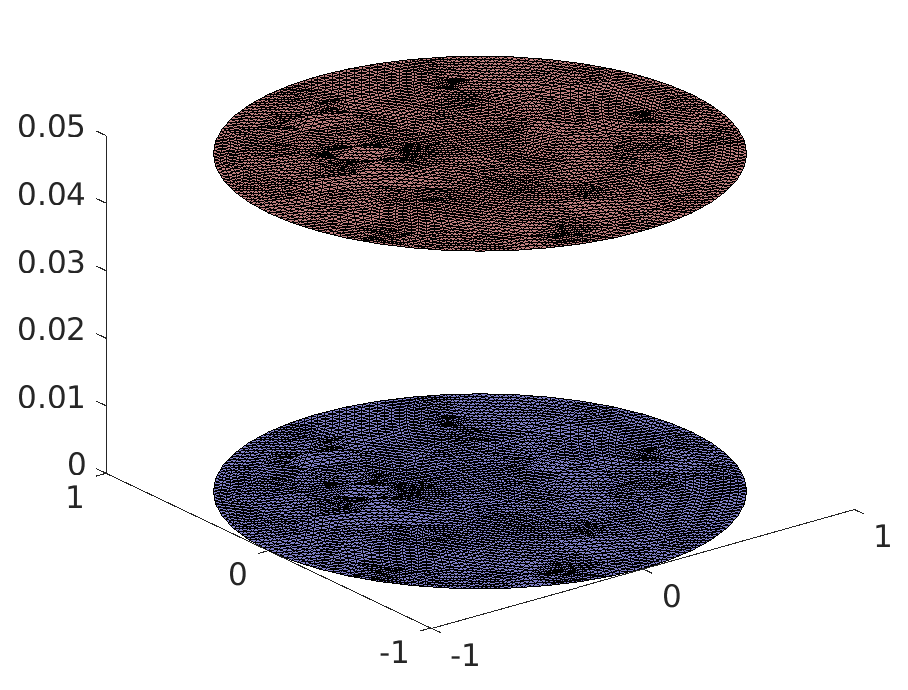
\includegraphics[width=0.48 \textwidth]{fig_article_chap_2/test_case_128/fig_u1u2_hmax0,09_Dt0,001_tt00.eps} 
\quad
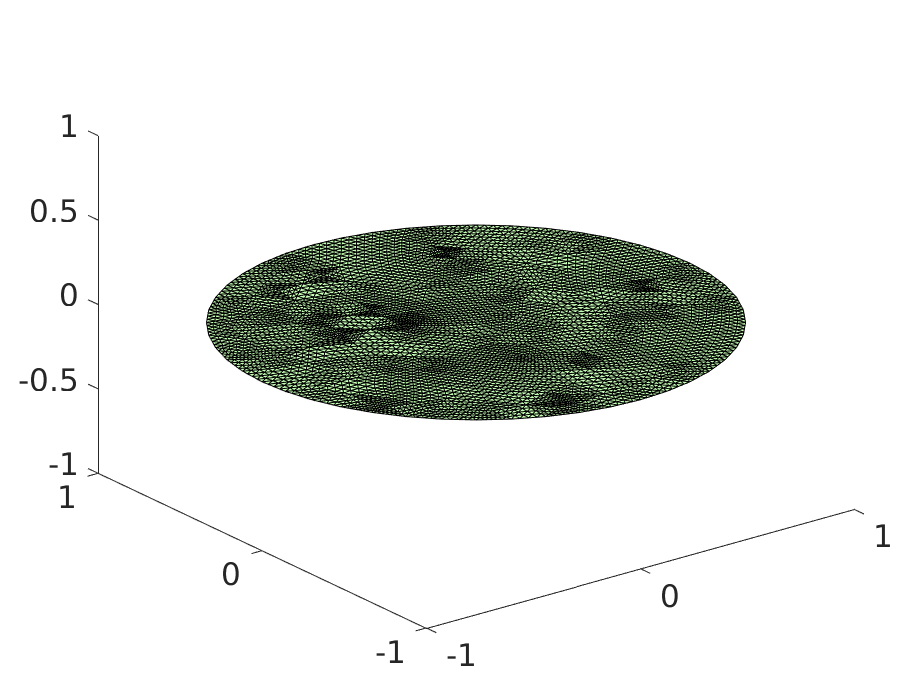
\includegraphics[width=0.48 \textwidth]{fig_article_chap_2/test_case_128/fig_lambda_hmax0,09_Dt0,001_tt02.eps} 
\end{figure}
\onslide<2>
\begin{figure}
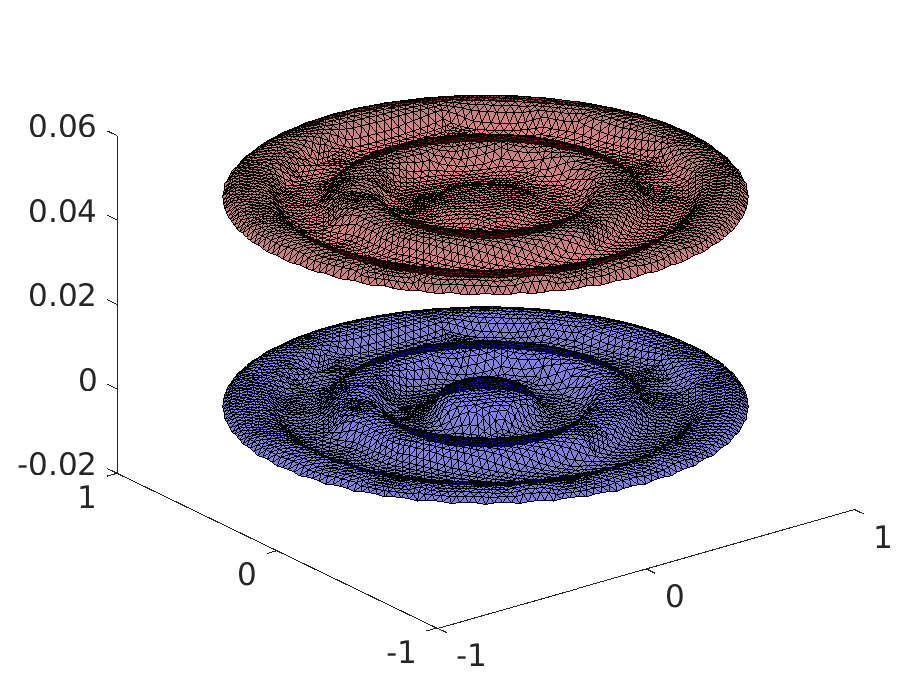
\includegraphics[width=0.48 \textwidth]{fig_article_chap_2/test_case_128/fig_u1u2_hmax0,09_Dt0,001_tt01.eps} 
\quad
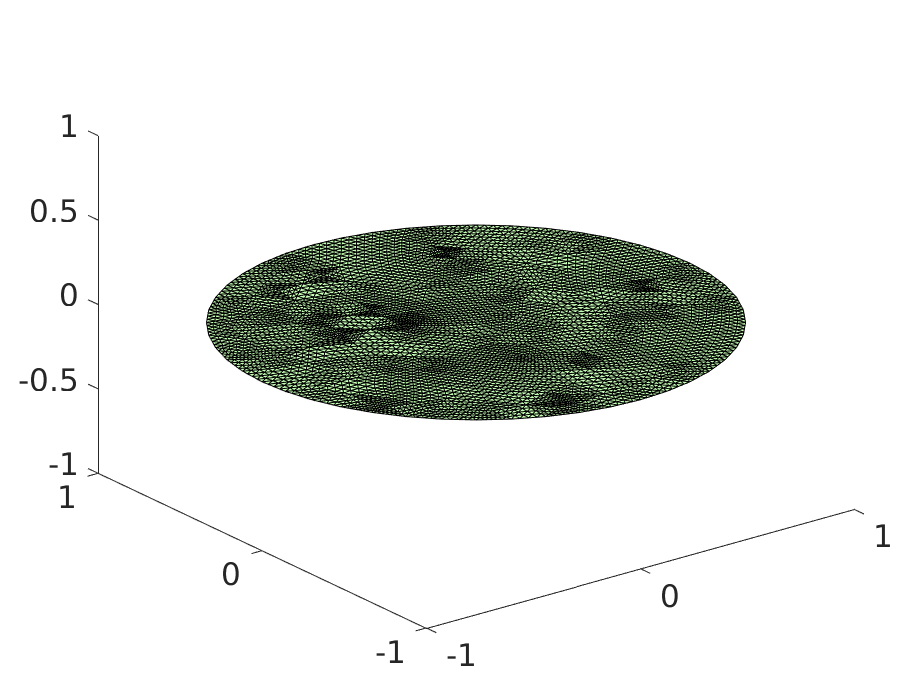
\includegraphics[width=0.48 \textwidth]{fig_article_chap_2/test_case_128/fig_lambda_hmax0,09_Dt0,001_tt02.eps} 
\end{figure}
\onslide<3>
\begin{figure}
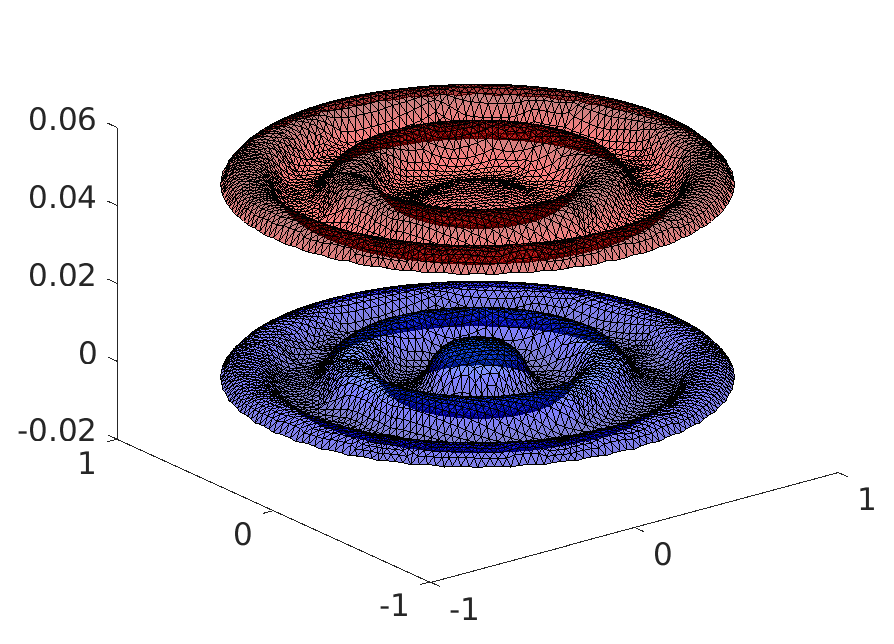
\includegraphics[width=0.48 \textwidth]{fig_article_chap_2/test_case_128/fig_u1u2_hmax0,09_Dt0,001_tt02.eps} 
\quad
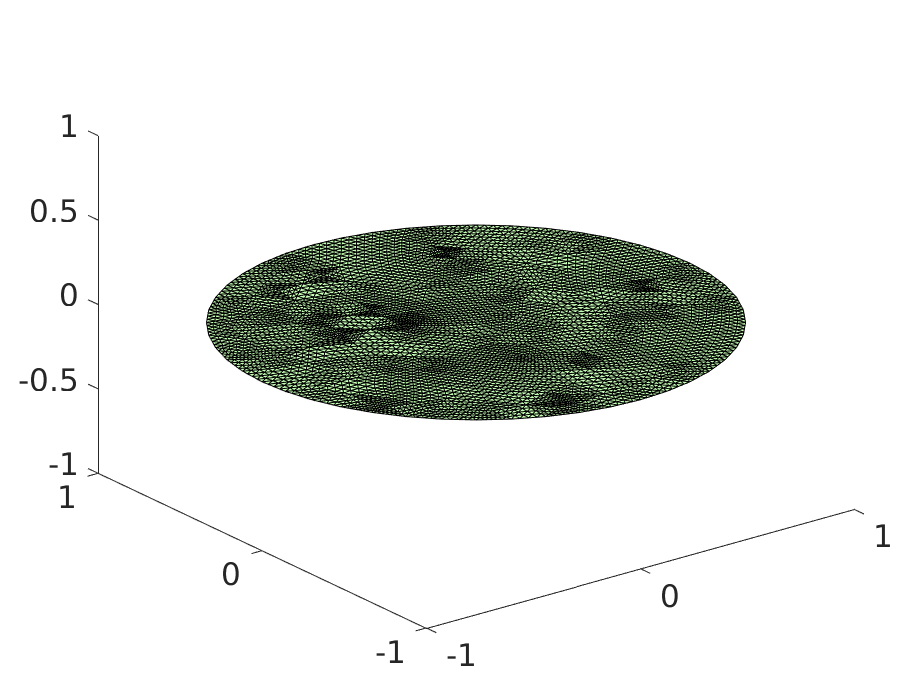
\includegraphics[width=0.48 \textwidth]{fig_article_chap_2/test_case_128/fig_lambda_hmax0,09_Dt0,001_tt02.eps} 
\end{figure}
\onslide<4>
\begin{figure}
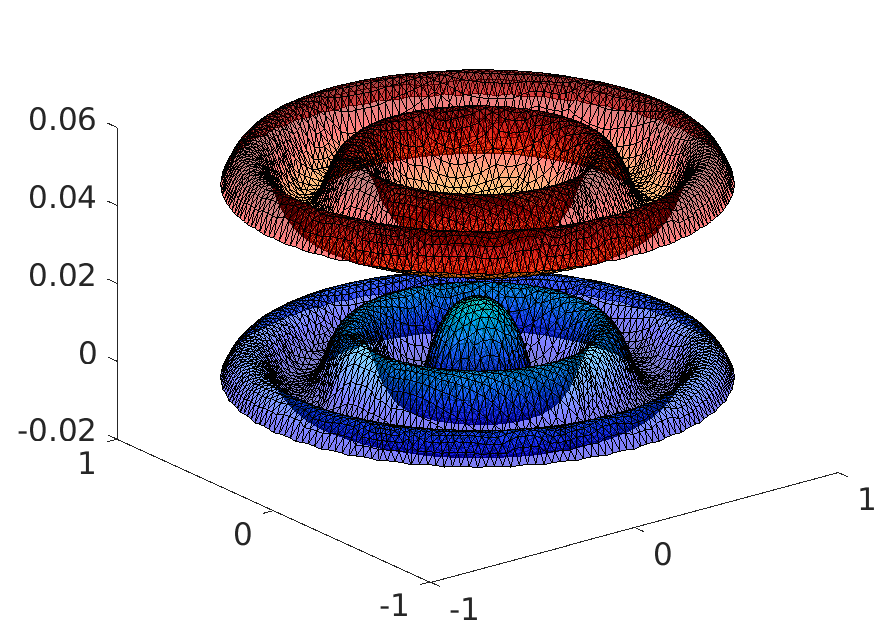
\includegraphics[width=0.48 \textwidth]{fig_article_chap_2/test_case_128/fig_u1u2_hmax0,09_Dt0,001_tt03.eps} 
\quad
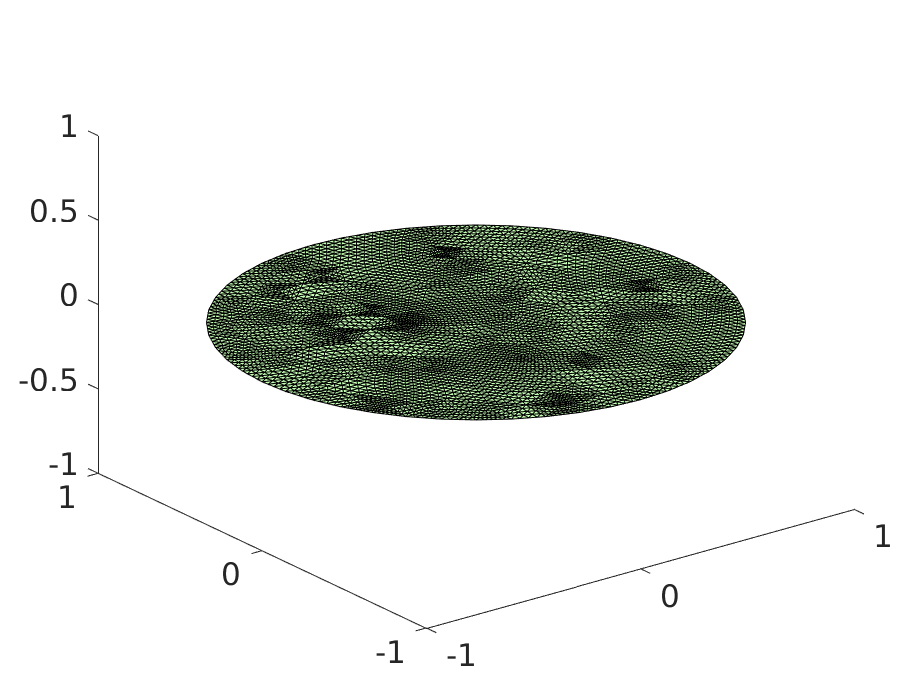
\includegraphics[width=0.48 \textwidth]{fig_article_chap_2/test_case_128/fig_lambda_hmax0,09_Dt0,001_tt02.eps} 
\end{figure}
\onslide<5>
\begin{figure}
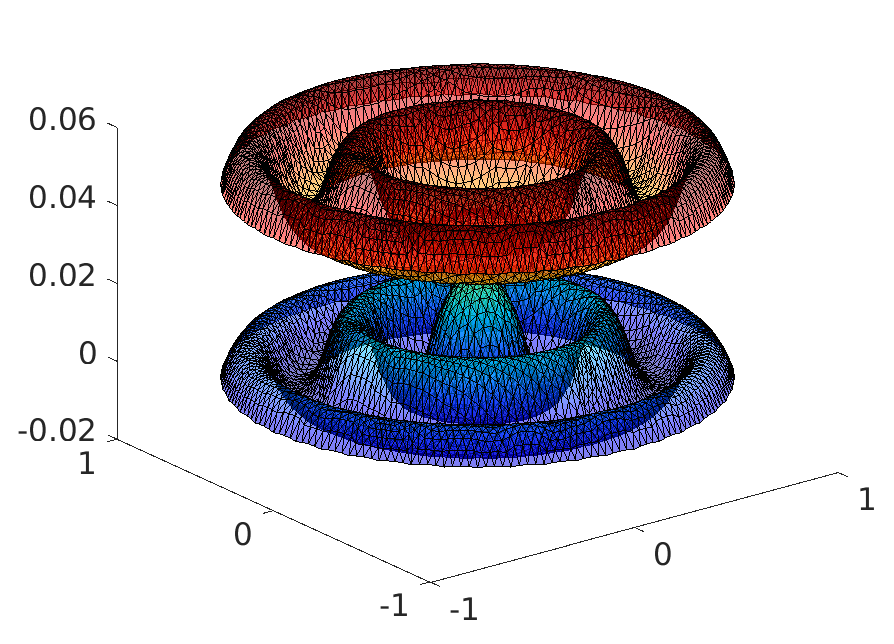
\includegraphics[width=0.48 \textwidth]{fig_article_chap_2/test_case_128/fig_u1u2_hmax0,09_Dt0,001_tt04.eps} 
\quad
\includegraphics[width=0.48 \textwidth]{fig_article_chap_2/test_case_128/fig_lambda_hmax0,09_Dt0,001_tt02.eps} 
\end{figure}
\onslide<6>
\begin{figure}
\includegraphics[width=0.48 \textwidth]{fig_article_chap_2/test_case_128/fig_u1u2_hmax0,09_Dt0,001_tt05.eps} 
\quad
\includegraphics[width=0.48 \textwidth]{fig_article_chap_2/test_case_128/fig_lambda_hmax0,09_Dt0,001_tt05.eps}
\end{figure}
\onslide<7>
\begin{figure}
\includegraphics[width=0.48 \textwidth]{fig_article_chap_2/test_case_128/fig_u1u2_hmax0,09_Dt0,001_tt06.eps} 
\quad
\includegraphics[width=0.48 \textwidth]{fig_article_chap_2/test_case_128/fig_lambda_hmax0,09_Dt0,001_tt06.eps} 
\end{figure}
\onslide<8>
\begin{figure}
\includegraphics[width=0.48 \textwidth]{fig_article_chap_2/test_case_128/fig_u1u2_hmax0,09_Dt0,001_tt07.eps} 
\quad
\includegraphics[width=0.48 \textwidth]{fig_article_chap_2/test_case_128/fig_lambda_hmax0,09_Dt0,001_tt07.eps} 
\end{figure}
\onslide<9>
\begin{figure}
\includegraphics[width=0.48 \textwidth]{fig_article_chap_2/test_case_128/fig_u1u2_hmax0,09_Dt0,001_tt08.eps} 
\quad
\includegraphics[width=0.48 \textwidth]{fig_article_chap_2/test_case_128/fig_lambda_hmax0,09_Dt0,001_tt08.eps} 
\end{figure}
\onslide<10>
\begin{figure}
\includegraphics[width=0.48 \textwidth]{fig_article_chap_2/test_case_128/fig_u1u2_hmax0,09_Dt0,001_tt09.eps} 
\quad
\includegraphics[width=0.48 \textwidth]{fig_article_chap_2/test_case_128/fig_lambda_hmax0,09_Dt0,001_tt09.eps} 
\end{figure}
\onslide<11>
\begin{figure}
\includegraphics[width=0.48 \textwidth]{fig_article_chap_2/test_case_128/fig_u1u2_hmax0,09_Dt0,001_tt10.eps} 
\quad
\includegraphics[width=0.48 \textwidth]{fig_article_chap_2/test_case_128/fig_lambda_hmax0,09_Dt0,001_tt10.eps} 
\end{figure}
\onslide<12>
\begin{figure}
\includegraphics[width=0.48 \textwidth]{fig_article_chap_2/test_case_128/fig_u1u2_hmax0,09_Dt0,001_tt11.eps} 
\quad
\includegraphics[width=0.48 \textwidth]{fig_article_chap_2/test_case_128/fig_lambda_hmax0,09_Dt0,001_tt11.eps} 
\end{figure}
\onslide<13>
\vspace*{-0.3 cm}
\begin{figure}
\includegraphics[width=0.48 \textwidth]{fig_article_chap_2/test_case_128/fig_u1u2_hmax0,09_Dt0,001_tt12.eps} 
\quad
\includegraphics[width=0.48 \textwidth]{fig_article_chap_2/test_case_128/fig_lambda_hmax0,09_Dt0,001_tt12.eps} 
\end{figure}
\onslide<14>
\begin{figure}
\includegraphics[width=0.48 \textwidth]{fig_article_chap_2/test_case_128/fig_u1u2_hmax0,09_Dt0,001_tt14.eps} 
\quad
\includegraphics[width=0.48 \textwidth]{fig_article_chap_2/test_case_128/fig_lambda_hmax0,09_Dt0,001_tt14.eps} 
\end{figure}
\end{overprint}
\end{frame}


\begin{frame}
\frametitle{Newton--Fischer--Burmeister adaptivity}
\textcolor{red}{\bm{$\gammalin=\gammaalg=10^{-3}$}}
\begin{figure}
\centering
\includegraphics[scale=0.43]{fig_article_chap_2/test_case_1_iter_11_estimator_gmres_1st_newton_iter}
\includegraphics[scale=0.43]{fig_article_chap_2/test_case_1_iter_11_estimator_newton_iter}
\end{figure}
\end{frame}

\begin{frame}
\frametitle{Newton--Fischer--Burmeister performance}
\vspace*{-0.2 cm}
\begin{figure}
\centering
% \includegraphics[width=0.48 \textwidth]{fig_article_chap_2/test_case_128/Number_Newton_FB_iter_time_gamma_10-3} 
\includegraphics[width=0.45 \textwidth]{fig_article_chap_2/test_case_128/Cumulated_number_Newton_FB_iter_time_gamma_10-3}
\quad
\includegraphics[width=0.45 \textwidth]{fig_article_chap_2/test_case_128/cumulated_number_gmresFB_iter_time_gamma_lin_alg_10-3}
\end{figure}
\vspace*{-0.2 cm}
\begin{thebibliography}{10}
 \scriptsize{
 \bibitem{Dabaghi:Martin:Vohralik:parabolic:2020}
 {\sc J.~Dabaghi, V.~Martin, M.~Vohral\'{i}k}, A posteriori estimates distinguishing the error components and
adaptive stopping criteria for numerical approximations of parabolic variational inequalities.
\em{Computer methods in applied mechanics and engeneering} (2020).
}
 \end{thebibliography}
\end{frame}
%

%% CHAP 3

\begin{frame}
  \frametitle{Two-phase flow with phase appearance and disappearance}
  \begin{minipage}{0.65 \textwidth}
  \textcolor{red}{\textbf{Storage of radioactive wastes in deep geological layers}}
\vspace*{-0.2 cm}
\begin{equation*}
\dps
\left\lbrace\begin{array}{llccc}
\dps \partial_t l_\componentw(\textcolor{cadmiumgreen}{\Sl}) + \nab \cdot {\bm \Phi}_{\mathrm{w}}(\textcolor{cadmiumgreen}{\Sl,\Pl,\chihl}) = Q_{\componentw}, \\
\dps \partial_t l_\componenth(\textcolor{cadmiumgreen}{\Sl,\Pl,\chihl})  + \nab \cdot {\bm \Phi}_{\mathrm{h}}(\textcolor{cadmiumgreen}{\Sl,\Pl,\chihl})=\Qh,\\
\textcolor{electricpurple}{1 - \Sl} \geq 0, \;  \textcolor{carmine}{H \Pg - \beta_{\phasel} \chihl} \geq 0, \; \left[\textcolor{electricpurple}{1 - \Sl} \right] \cdot \left[\textcolor{carmine}{H \Pg - \beta_{\phasel} \chihl}\right]=0   \\
\Sl(\cdot, 0) = \Sl_0, \quad \Pl(\cdot, 0) = \Pl_0, \quad \chihl(\cdot, 0) = \chi_{\mathrm{h}, 0}^{\mathrm{l}} \\
{\bm \Phi}_{\mathrm{w}}\cdot \bn_{\Omega} = 0, \quad {\bm \Phi}_{\mathrm{h}}\cdot \bn_{\Omega} = 0 
\end{array}
\right.
\end{equation*}
  \end{minipage}
  \hfill
  \begin{minipage}{0.34 \textwidth}
\includegraphics[scale = 0.6]{stockage_radioactifs}
    \end{minipage}
\vspace{0.1 cm}
\invisible<1>{
\textcolor{midnightblue}{\textbf{Unknowns:}} liquid saturation $\textcolor{cadmiumgreen}{\Sl}$, liquid pressure $\textcolor{cadmiumgreen}{\Pl}$, mole fraction of liquid hydrogen $\textcolor{cadmiumgreen}{\chihl}$ \\
\vspace{0.3 cm}
\invisible<2>{
\textcolor{midnightblue}{\textbf{Linear functions:}} amount of water $l_\componentw$, amount of hydrogen $l_\componenth$\\
\vspace{0.3 cm}
\invisible<3>{
\textcolor{midnightblue}{\textbf{Nonlinear fluxes:}} water flux $\underbrace{{\bm \Phi}_{\mathrm{w}}}_{\mathrm{Darcy} + \mathrm{Fick}}$, hydrogen flux $\underbrace{{\bm \Phi}_{\mathrm{h}}}_{\mathrm{Darcy} + \mathrm{Fick}}$\\
\vspace{0.3 cm}
\invisible<4>{
\textcolor{midnightblue}{\textbf{Nonlinear complementarity constraints:}} $\Rightarrow$ \textbf{Phase change}\\
\vspace{0.2 cm}
\scriptsize{Ben Gharbia and Jaffré (2014)}

\invisible<5>{
}}}}}

\end{frame}
%

%
%% DISCRETIZATION FINITE VOLUME
% \begin{frame}
% \frametitle{Discretization by the finite volume method}
% \textcolor{blue}{\textbf{Numerical solution: }}
% \begin{equation*}
% \bUn \egaldef (\bUn_K)_{K\in \Th}, \qquad \bUn_K \egaldef  (\SKn,\PKn,\chiKn) \quad \textcolor{cadmiumgreen}{\textbf{one value per cell and time step}} 
% \label{eq:finite:volume:approx}
% \end{equation*}
% \textcolor{cadmiumgreen}{\textbf{Time discretization:}}
% \\
%  \begin{figure}[htbp]
% \vspace{-0.6 cm}
%  \centering
%  \begin{picture}(200,60)(0,0)
%  \thicklines
%  \put(0,15){\line(200,0){200}}
%  %\put(0,10){\red{\line(0,10){10}}}
%  \put(0,0){\makebox(0,0){\small \red{$t_0 = 0$}}}
%  \put(0,15){\black{\circle*{6}}}
%  \put(25,10){\red{\line(0,10){10}}}
%  \put(25,0){\makebox(0,0){\small \red{$t_1$}}}
%  %\put(25,15){\blue{\circle*{6}}}
%  \put(12.5,30){\makebox(0,0){\small  \blue{$I_1$}}}
%  \put(50,10){\red{\line(0,10){10}}}
%  \put(50,0){\makebox(0,0){\small \red{$t_2$}}}
%  %\put(75,15){\blue{\circle*{6}}}
%  \put(37.5,30){\makebox(0,0){\small  \blue{$I_2$}}}
%  \put(75,30){\makebox(0,0){\small \blue{$\cdots$}}}
%  \put(75,0){\makebox(0,0){\small \red{$\cdots$}}}
%  \put(112.5,30){\makebox(0,0){\small \blue{$I_{n}$}}}
%  %\put(215,15){\blue{\circle*{6}}}
%  \put(100,10){\red{\line(0,10){10}}}
%  \put(100,0){\makebox(0,0){\red{\small $t_{n-1}$}}}
%  \put(125,10){\red{\line(0,10){10}}}
%  \put(125,0){\makebox(0,0){\red{\small $t_{n}$}}}
%  \put(150,30){\makebox(0,0){\small \blue{$\cdots$}}}
%  \put(150,0){\makebox(0,0){\small \red{$\cdots$}}}
%  \put(175,0){\makebox(0,0){\small \red{$t_{\Nt - 1}$}}}
%  \put(175,10){\red{\line(0,10){10}}}
%  %\put(355,15){\blue{\circle*{6}}}
%  \put(187.5,30){\makebox(0,0){\small \blue{$I_{\Nt}$}}}
%  \put(200,0){\makebox(0,0){\small \red{$t_{\Nt} = t_{\mathrm{F}}$}}}
%  %\put(240,10){\red{\line(0,10){10}}}
%  \put(200,15){\black{\circle*{6}}}
%  \end{picture}
% \qquad \qquad
% \includegraphics[scale = 0.5]{fig_article_chap_2/approx_time_derivative.pdf}
%  \end{figure}
% \begin{minipage}[c]{0.3 \textwidth}
% \textcolor{cadmiumgreen}{\textbf{Space discretization:}} $\Th$ a superadmissible family of conforming simplicial meshes of $\Omega$. \textcolor{blue}{Number of cells : $\Nsp$}
% \begin{equation*}
% \dps 
% \left(\nab v \cdot \bn_{K,\sigma},1\right)_{\sigma} := \dps |\sigma| \frac{v_L - v_K}{d_{KL}} \hspace{0.2 cm} \sigma = \overline{K} \cap \overline{L},
% \end{equation*}
% \end{minipage}
% \hfill
% \begin{minipage}[c]{0.5 \textwidth}
% \begin{figure}
% \includegraphics[width = 0.7 \textwidth]{fig_article_chap_3/gradient_discretization.pdf}
% \end{figure}
% \end{minipage}
% \end{frame}

\begin{frame}
\frametitle{Discretization by the finite volume method}
\textcolor{cadmiumgreen}{\textbf{Numerical solution: }}
\begin{equation*}
 \bUn \egaldef (\bUn_K)_{K\in \Th}, \qquad \bUn_K \egaldef  (\SKn,\PKn,\chiKn) \quad \textcolor{cadmiumgreen}{\textbf{one value per cell and time step}} 
\end{equation*}
\textcolor{blue}{\textbf{Discretization of the water equation}}
\begin{equation*}
S_{\mathrm{w},K}^n(\bU^n) \egaldef |K| \partial_t^n \lwK  + \sum_{\sigma \in \EK} {F}_{\componentw,K,\sigma}(\bU^{n})- |K|\QwKn = 0,
\end{equation*}
% \begin{equation*}
% {F}_{\componentw,K,\sigma}(\bUn) \egaldef \rhowl (\mobilityliq)_{\sigma}^{n} (\psil)_{\sigma}^{n} - (\jhl)_{\sigma}^{n} \quad \sigma \in \EKint \quad \overline{\sigma} = \overline{K} \cap \overline{L}.
% \end{equation*}
\invisible<1>{
\textcolor{blue}{\textbf{Discretization of the hydrogen equation}}
\begin{equation*} 
S_{\mathrm{h},K}^{n}(\bU^n)\egaldef |K| \partial_t^n \lhK + \sum_{\sigma \in \EK} {F}_{\componenth,K,\sigma}(\bUn) - |K| \QhKn = 0,
\end{equation*}
% \begin{equation*}
%  {F}_{\componenth,K,\sigma}(\bUn) \egaldef \betal \chisigman (\mobilityliq)_{\sigma}^{n} (\psil)_{\sigma}^{n} + (\psig)_{\sigma}^{n} (\mobilitygas)_{\sigma}^{n} (\rhog)_{\sigma}^{n} + (\jhl)_{\sigma}^{n} , \quad \sigma \in \EKint \quad \overline{\sigma} = \overline{K} \cap \overline{L}.
% \end{equation*}
\invisible<2>{
At each time step $t^n$, we obtain the nonlinear system of algebraic equations
\begin{equation*}
S_{c,K}^n(\bU^n)=0 \quad \forall K \in \Th \ \ \forall \componentc \in \left\{\componentw,\componenth\right\}
\end{equation*}
\invisible<3>{
}}}
\end{frame}
%
\begin{frame}
\frametitle{Discrete complementarity problem and semismoothness}
\textcolor{red}{\textbf{Discretization of the nonlinear complementarity constraints}}
\begin{equation*}
\textcolor{electricpurple}{\mathcal{K}(\bU_K^n)} \egaldef \textcolor{electricpurple}{1-\SKn} \quad \textcolor{carmine} {\mathcal{G}(\bU_K^n)} \egaldef  \textcolor{carmine}{H(\PKn\hspace{-0.05 cm}+\hspace{-0.05 cm}\Pcp(\SKn))-\betal \chiKn}
\end{equation*}
\pause
The discretization reads
\begin{equation*}
\begin{split}
&S_{c,K}^n(\bU^n)=0 \quad \forall K \in \Th \quad \forall \componentc \in \left\{\componentw,\componenth \right\}\\
& \textcolor{electricpurple}{\mathcal{K}(\bU_K^n)} \geq 0, \quad   \textcolor{carmine} {\mathcal{G}(\bU_K^n)} \geq 0, \quad \textcolor{electricpurple}{\mathcal{K}(\bU_K^n)} \cdot \textcolor{carmine} {\mathcal{G}(\bU_K^n)}=0 \quad \forall K \in \Th
\end{split}
\end{equation*}
\pause
\begin{itemize}
\item
\textcolor{cadmiumgreen}{\textbf{We reformulate the complementarity constraints with C-functions}}
\item
\textcolor{cadmiumgreen}{\textbf{We employ inexact semismooth linearization}}
\item
\textcolor{cadmiumgreen}{\textbf{Can we estimate the error?}}
\item
\textcolor{cadmiumgreen}{\textbf{Can we distinguish the error components?}}
\end{itemize}
\end{frame} 
%
%%
\begin{frame}
  \frametitle{A posteriori analysis}
  \textcolor{red}{\textbf{Assumption: There exists a unique weak solution satisfying}}
\begin{equation*}
X \egaldef L^2((0,\tF);H^1(\Omega)), \ Y  \egaldef H^1((0,\tF);L^2(\Omega)), 
%\ \widehat{Y} \egaldef H^1((0,\tF);L^{\infty}(\Omega)),\\
 \  Z \egaldef L_{+}^2((0,\tF);L^{\infty}(\Omega)) 
% \\ & \left\| \varphi \right\|_{X_n} \egaldef \int_{\In} \sum_{K \in \Th} \left(\varepsilon h_K^{-2} \left\|\varphi\right\|_K^2 + \left\|\nab \varphi\right\|_K^2\right) (t) \mathrm{dt}
\end{equation*}
\begin{itemize}
\item
% $\Sl \in \widehat{Y}$, \ 
$\textcolor{electricpurple}{1-\Sl} \in Z$, \ $\lc \in Y$, \ $\Pl \in X$, \ $\chihl \in X$, \ $\Phic \in L^2((0,\tF); \HdivOmeg)$
\item 
$\dps \int_{0}^{\tF} \left(\partial_t \lc, \varphi \right)_{\Omega}(t)\,\mathrm{dt}-\hspace{-0.1 cm}\int_{0}^{\tF} \left(\Phic, \nab \varphi \right)_{\Omega}(t)\,\mathrm{dt} = \hspace{-0.1 cm} \int_{0}^{\tF} \left(\Qc, \varphi \right)_{\Omega}(t)\,\mathrm{dt} \quad \forall \varphi \in X$
\item 
$\dps \int_{0}^{\tF} \left(\lambda - \left(\textcolor{electricpurple}{1 - \Sl}\right), \textcolor{carmine}{H[\Pl+\Pcp(\Sl)]-\betal \chihl}  \right)_{\Omega}(t)\,\mathrm{dt} \geq 0 \quad \forall \lambda \in Z$
\item
the initial condition holds
\end{itemize}
\textcolor{red}{\textbf{Error measure:}} Dual norm of the residual $+$ residual for the complementarity constraints $+$ nonconformity of pressure and molar fraction.
\\
\textcolor{red}{\textbf{Adaptivity:}} construct estimators and distinguish the error components

\end{frame}
% 
\begin{frame}
\frametitle{Numerical experiments}
$\Omega$:  one-dimensional core with length $L = 200 m$. 
\\
\vspace{0.2 cm}
\textbf{Semismooth solver:} Newton-min
\\
\vspace{0.2 cm}
\textbf{Iterative algebraic solver:} GMRES.
\\
\vspace{0.2 cm}
\textbf{Time step:} $\Delta t = 5000$ years, 
\\
\vspace{0.2 cm}
\textbf{Number of cells:} $\Nsp = 1000$, \\
\vspace{0.2 cm}
\textbf{Final simulation time:} $\tF = 5 \times 10^{5}$ years.
\\
\vspace{0.2 cm}
\begin{figure}
\includegraphics[width= 1 \textwidth]{fig_article_chap_3/num_exp_finite_vol}
\end{figure}

\end{frame}
% 

\begin{frame}
\frametitle{Phase transition estimator}

  \begin{overprint}
    \onslide<1> \scriptsize{\textcolor{red}{\textbf{\bm{$t=2500$} years}}} 
\begin{figure}
\includegraphics[width=0.47\textwidth]{fig_article_chap_3/satur_gas_init_time2}
\quad
\includegraphics[width=0.47\textwidth]{fig_article_chap_3/MODIF_phase_transition_estimator_appearance_gas_nt=inittime_cv} 
    \end{figure}
\onslide<2>
\scriptsize{\textcolor{red}{ \textbf{\bm{$t = 1.25 \times 10^4$} years}}}
\begin{figure}
\includegraphics[width=0.45\textwidth]{fig_article_chap_3/satur_gas_appearance.eps}
 \quad
\includegraphics[width=0.47\textwidth]{fig_article_chap_3/MODIF_phase_transition_estimator_appearance_gas_nt=2_cv}
\end{figure}    

\onslide<3>
\scriptsize{ \textbf{\textcolor{red}{ \bm{$t = 4.25 \times 10^4$} years}}}
\begin{figure}
\includegraphics[width=0.45\textwidth]{fig_article_chap_3/satur_gas_after_appearance.eps}
\quad
\includegraphics[width=0.47\textwidth]{fig_article_chap_3/MODIF_phase_transition_estimator_appearance_gas_nt=9_cv}
\end{figure}
\end{overprint}
 \end{frame}
%
\begin{frame}
\frametitle{Overall performance $\gammalin = \gammaalg = 10^{-3}$}
\begin{figure}
\centering
\includegraphics[width=0.47\textwidth]{fig_article_chap_3/Cumulated_number_Newton_iterations_three_methods_Nx_1000}
\hspace{0.6 cm}
\includegraphics[width=0.47\textwidth]{fig_article_chap_3/Cumulated_number_gmres_iterations_three_methods_Nx_1000}
\end{figure}
\end{frame}
%
\begin{frame}
\frametitle{Accuracy $\gammalin = \gammaalg = 10^{-3}$}
\vspace{-0.1 cm}
\textcolor{cadmiumgreen}{\hspace{2 cm} $t = 1.05 \times 10^5$ years \hspace{5 cm} $t = 3.5 \times 10^5$ years}
\begin{figure}
\centering
\includegraphics[width=0.48 \textwidth]{fig_article_chap_3/comparaison_plot_gas_saturations_exact_adapt_inexact_gamma_lin_gamma_alg_10-3_nt_21}
\includegraphics[width=0.48 \textwidth]{fig_article_chap_3/comparaison_plot_gas_saturations_exact_adapt_inexact_gamma_lin_gamma_alg_10-3_nt_70}
\end{figure}
\begin{thebibliography}{10}
 \scriptsize{
 \bibitem{Dabaghi:Martin:Vohralik:BenGharbia:2020}
 {\sc I.~Ben Gharbia J.~Dabaghi, V.~Martin, M.~Vohral\'{i}k}, A posteriori error estimates for a compositional two-phase flow
with nonlinear complementarity constraints.
\em{Computational Geosciences} (2020).
}
 \end{thebibliography}
\end{frame}

%

%% CONCLUSION
\section{Conclusion}
\subsection{}

%%% CONCLUSION



\begin{frame}
\frametitle{Conclusion and perspectives}
\textcolor{midnightblue}{\large \textbf{Conclusion}}
\invisible<1>{
\begin{itemize}
\item
We proposed several numerical schemes for variational inequalities. 
\item We devised a posteriori error estimates with $\Pp$ finite elements distinguishing the error components.
\item
Adaptive stopping criteria $\Rightarrow$ reduction of the number of iterations.
\item
 Our a posteriori analysis works for unsteady problems (Two-phase flow with phase transition). 
\end{itemize}
\invisible<2>{
\textcolor{midnightblue}{\large \textbf{Perspectives}}
\begin{itemize}
\item Extension of the stationary contact problem to a hyperbolic contact problem between two vibrating membranes.
\item
Devise a posteriori error estimators for HHO
\item
Construct a posteriori error estimates for a multiphase multi compositional flow with several phase transitions.
\end{itemize}
\invisible<3>{
}}}
\end{frame}
%

%% REMERCIEMENTS + SLIDE RESERVE
\begin{frame}
\begin{overprint}

\onslide<1>
\vspace{0.3 cm}
\begin{center}
\LARGE{\textcolor{midnightblue}{Acknowledgements}}
\end{center}
\begin{itemize}
\item 
Martin Vohral\'{i}k (INRIA Paris)
\item
Vincent Martin (UTC Compiègne)
\item 
 Ibtihel Ben Gharbia (IFPEN)
 \item 
 Guillaume Delay (LJLL)
 \item 
 Soleiman Yousef (IFPEN)
 \item 
 Jean-Charles Gilbert (INRIA Paris)
\end{itemize}
\vspace*{0.2 cm}
\begin{center}
\Huge{\textcolor{black}{Thank you for your attention}}
\end{center}

%%%%%
   \onslide<2> 

\textcolor{cadmiumgreen}{\textbf{Discretization flux reconstruction:}}
\begin{equation*}
\begin{array}{lclcc}
\left({\bm \sigma}_{\ialf h, \mathrm{disc}}^{\kk,\ii,\ba}, \tauh\right)_{\omah}- \left(\gamma_{\ialf h}^{\kk,\ii,\ba},\nab {\cdot} \tauh\right)_{\omah}
&=& -\left(\mu_\ialf \psiha \nab u_{\ialf h}^{\kk,\ii,\ba}, \tauh \right)_{\omega_h^{\ba}}
&  \forall \tauh\in \Vspaceha, \\
\left(\nab {\cdot} {\bm \sigma}_{\ialf h, \mathrm{disc}}^{\kk,\ii, \ba}, q_{h}\right)_{\omah}
&=&\left(\tilde{g}_{\ialf h}^{\kk,\ii,\ba}, q_{h}\right)_{\omah}
&  \forall q_{h}\in \Qspaceha,
\end{array}
\end{equation*}
\begin{equation*}
\tildgialfhkia \egaldef \left(f_\ialf -(-1)^{\ialf} \tildlambhkia -\rialfhki \right) \psiha- \mu_\ialf \nab \uialfhki {\cdot} \nab \psiha : \mbox{\textcolor{cadmiumgreen}{depends on the residual}} 
%\left(f_\ialf -(-1)^{\ialf} \tildlambhkia -\rialfhki \right) \psiha- \mu_\ialf \nab \uialfhki {\cdot} \nab \psiha
\end{equation*}
\begin{minipage}[c]{0.4 \linewidth}
For each internal vertex $ \ba \in \Vhint$
\vspace{-0.2 cm}
\begin{equation*}
\begin{split}
\Vspaceha & \egaldef
 \left\{\tauh  \in \RTp(\omah), \, \tauh {\cdot} \nnomah=0  \mbox{ on } \partial \omah \right\}\\
\Qspaceha &  \egaldef \Pp^{0}(\omah)
\end{split}
\vspace{-0.2 cm}
\end{equation*}

\invisible<1>{
\begin{equation*}
{\bm \sigma}_{\ialf h, \mathrm{disc}}^{\kk,\ii} \egaldef \sum_{\ba \in \mathcal{V}_h} {\bm \sigma}_{\ialf h, \mathrm{disc}}^{\kk,\ii,\ba}
\end{equation*}
}
\end{minipage}
\hfill
\begin{minipage}[c]{0.5 \linewidth}
\begin{figure}
  %\begin{overprint}
    %\onslide<1>\includegraphics[width=0.84\textwidth]{patch_alg_3.pdf}
    \includegraphics[width=0.84\textwidth]{patch_alg_5.pdf}
   % \end{overprint}
\end{figure}
\end{minipage}

\onslide<3>

\vspace{0.2 cm}
\textcolor{cadmiumgreen}{\textbf{Strategy for constructing the estimators}}
\begin{equation*}
%\label{eq:def:lambda:pos:neg}
\lambh^{\kk,\ii} \egaldef \lambh^{\kk,\ii,\mathrm{pos}} + \lambh^{\kk,\ii,\mathrm{neg}}, \quad \Ktildeghp \egaldef \left\{(\vunh,\vdeuxh) \in \Xghp \times \Xzerohp, \ \textcolor{electricpurple}{\vunh-\vdeuxh} \geq 0  \right\} \subset \Kg.
\end{equation*}
\textcolor{midnightblue}{\textbf{Nonconformity estimator 1:}}
\begin{equation*}
\eta_{\mathrm{nonc},1,K}^{\kk,\ii}  \egaldef  \tnorm{{\bm s}_h^{\kk,\ii}-\uh^{\kk,\ii}}_K, 
\end{equation*}
\vspace{-0.1 cm}
\textcolor{midnightblue}{\textbf{Nonconformity estimator 2:}}
\begin{equation*}
\eta_{\mathrm{nonc},2,K}^{\kk,\ii} \egaldef h_{\Omega} \CPF \left(\frac{1}{\mu_1} +
\frac{1}{\mu_2} \right)^{\frac{1}{2}} \left\| \lambh^{\kk,\ii,\mathrm{neg}}\right\|_K, 
\end{equation*}
\vspace{-0.2 cm}
\textcolor{midnightblue}{\textbf{Nonconformity estimator 3:}}
\begin{equation*}
\eta_{\mathrm{nonc},3,K}^{\kk,\ii}  \egaldef 2 h_{\Omega} \CPF \left(\frac{1}{\mu_1} +
\frac{1}{\mu_2} \right)^{\frac{1}{2}} \left\|\lambh^{\kk,\ii,\mathrm{pos}}\right\|_{\Omega}
\tnorm{{\bm s}_{h}^{\kk,\ii}-\uh^{\kk,\ii}}_K.
\end{equation*}

%%%%%%%

\onslide<4>
\textcolor{cadmiumgreen}{\textbf{Distinguishing the error components}}
\\
\textcolor{midnightblue}{\textbf{$p=1$}}
\vspace*{-0.6 cm}
\small{
\begin{equation*}
  \begin{split}
  \eta_{\mathrm{disc}}^{\kk,\ii} & := \left\{\sum_{\alpha=1}^2 \sum_{K \in \Th} \left(\eta_{\mathrm{disc},K,\alpha}^{\kk,\ii} + \eta_{\mathrm{osc},K,\alpha} \right)^2  \right\}^{\frac{1}{2}} + \left\{|\sum_{K \in \Th} \eta_{\mathrm{C},K}^{\kk,\ii,\mathrm{pos}} |  \right\}^{\frac{1}{2}} \\
  \eta_{\mathrm{lin}}^{\kk,\ii} & := \eta_{\mathrm{nonc}, 1}^{\kk,\ii} + \eta_{\mathrm{nonc}, 2}^{\kk,\ii} + \left(\eta_{\mathrm{nonc}, 3}^{\kk,\ii} \right)^{\frac{1}{2}}, \quad   \eta_{\mathrm{alg}}^{\kk,\ii} := \left\{\sum_{\alpha=1}^2 \sum_{K \in \Th} \left\| \mu_{\alpha}^{-\frac{1}{2}} {\bm \sigma}_{\alpha h, \mathrm{alg}}^{\kk,\ii} \right\|_K^2 \right\}^{\frac{1}{2}}
  \end{split}
\end{equation*}
\vspace*{-0.4 cm}
\textcolor{midnightblue}{\textbf{$p \geq 2$}}
\vspace*{-0.3 cm}
\begin{equation*}
  \begin{split}
    \eta_{\mathrm{disc}}^{\kk,\ii} & := \left\{\sum_{\alpha=1}^2 \sum_{K \in \Th} \left(\eta_{\mathrm{disc},K,\alpha}^{\kk,\ii} + \eta_{\mathrm{osc},K,\alpha} \right)^2  \right\}^{\frac{1}{2}}
    + \left\{2 |\left(\lambda_h^{\kk,\ii,\mathrm{pos}} - \lambda_h^{\kk,\ii}, u_{1h}^{\kk,\ii} - u_{2h}^{\kk,\ii} \right)_{\Omega} |  \right\}^{\frac{1}{2}} \\
    & + \tnorm{\tilde{\bs}_h^{\kk,\ii} - {\bs}_h^{\kk,\ii}}
    + C_{\Omega,\mu} \left\| \lambda_h^{\kk,\ii,\mathrm{neg}} - \tilde{\lambda}_{h}^{\kk,\ii,\mathrm{neg}} \right\|_{\Omega} + \left(2 C_{\Omega,\mu} \left\|\lambda_h^{\kk,\ii,\mathrm{pos}} \right\|  \right)^{\frac{1}{2}} \tnorm{\tilde{\bs}_h^{\kk,\ii} - {\bs}_h^{\kk,\ii}}^{\frac{1}{2}}\\
    \eta_{\mathrm{lin}}^{\kk,\ii} & := \tnorm{{\bs}_h^{\kk,\ii} - {\bu}_h^{\kk,\ii}} + C_{\Omega,\mu} \left\| \tilde{\lambda}_{h}^{\kk,\ii,\mathrm{neg}} \right\|_{\Omega} + \left(2 C_{\Omega,\mu} \left\|\lambda_h^{\kk,\ii,\mathrm{pos}} \right\|  \right)^{\frac{1}{2}}  \tnorm{{\bs}_h^{\kk,\ii} - {\bu}_h^{\kk,\ii}}^{\frac{1}{2}}
    \\
    & + \left\{2 |\left(\lambda_h^{\kk,\ii}, u_{1h}^{\kk,\ii} - u_{2h}^{\kk,\ii} \right)_{\Omega} | \right\}^{\frac{1}{2}}
  \end{split}
\end{equation*}
}
\onslide<5>

\vspace{0.1 cm}
\textcolor{cadmiumgreen}{\textbf{Parabolic weak formulation}}
\\\\
\textcolor{midnightblue}{\textbf{Weak formulation:}} 
For $\left(f_1,f_2\right) \in  [L^2(0,T;L^2(\Omega))]^2$, $\bu^0 \in H_g^1(\Omega) \times H_0^1(\Omega)$, 
find  $(u_1,u_2,\lambda) \in L^2(0,T;H_g^1(\Omega)) \times L^2(0,T;H_0^1(\Omega)) \times L^2(0,T; \Lambda)$ s.t. $\dps \partial_t \uialf \in L^2(0,T;H^{-1}(\Omega))$, and satisfying $\forall t \in \left]0,T\right[$ 
\begin{equation*}
\vspace{-0.2 cm}
\begin{split}
&\sum_{\ialf=1}^2 \langle \partial_t \uialf(t), \vialf \rangle + \sum_{\ialf=1}^2 \mu_\ialf \left(\nab \uialf(t), \nab \vialf \right)_{\Omega} - \left(\lambda(t),v_1-v_2\right)_{\Omega} = \sum_{\ialf=1}^2 \left(f_\ialf, \vialf \right)_{\Omega}, \hspace{0.15 cm} \forall \bv \in \left[H_0^1(\Omega)\right]^2 \\
& \left(\chi-\textcolor{carmine}{\lambda(t)}, \textcolor{electricpurple}{u_1(t)-u_2(t)}\right)_{\Omega} \geq 0 \quad \forall \chi \in \Lambda.
\end{split}
\end{equation*}
\textcolor{midnightblue}{\textbf{Discrete formulation:}}
Given $\left(u_{1h}^0,u_{2h}^0 \right) \in \Kgh^{p}$, search $(\uunhn,\udeuxhn,\lambh^n)\in \Xghp \times \Xzerohp \times
\Lahp$ such that for all $\left(z_{1h},z_{2h},\chi_h\right) \in \Xzerohp \times \Xzerohp \times \Lahp$ 
\begin{equation*}
\begin{array}{lcl}
\dps \frac{1}{\Dt_n} \sum_{\ialf=1}^2 \left(\uialfhn-\uialfh^{n-1}, z_{\ialf h}\right)_{\Omega} + \sum_{\ialf=1}^2 \mu_\ialf \left(\nab u_{\ialf h}^n, \nab z_{\ialf h}\right)_{\Omega}
- \left\langle \lambh^n, z_{1h}-z_{2h} \right \rangle_h
=  \dps \sum_{\ialf=1}^2 \left(f_\ialf,z_{\ialf h}\right)_{\Omega}, \\
\left\langle \chi_h - \textcolor{carmine}{\lambh^n}, \textcolor{electricpurple}{\uunh^n - \udeuxh^n}\right \rangle_h   \geq 0 
\end{array}
\end{equation*}

\onslide<6>
\vspace{0.2 cm}
\textcolor{red}{$\bm \gammalin= \bm \gammaalg \bm = {\bm {10^{-6}}}$}
\\\\
\textcolor{cadmiumgreen}{\hspace{2 cm} $t = 1.05 \times 10^5$ years \hspace{5 cm} $t = 3.5 \times 10^5$ years}
\begin{figure}
\centering
\includegraphics[width=0.48 \textwidth]{fig_article_chap_3/comparaison_plot_gas_saturations_exact_adapt_inexact_gamma_lin_10-6_gamma_alg_10-3_nt_21}
\includegraphics[width=0.48 \textwidth]{fig_article_chap_3/comparaison_plot_gas_saturations_exact_adapt_inexact_gamma_lin_gamma_alg_10-3_nt_70}
\end{figure}

 \end{overprint} 

\end{frame}




% \bibliographystyle{plain}
% \bibliography{diphasique_biblio}
\end{document}



